\documentclass{article}
\usepackage[utf8]{inputenc}
\usepackage[margin=1in]{geometry}
\usepackage{soul,color}
\usepackage{amsfonts, amsmath}
\usepackage{bbm}
\usepackage{enumitem}
\newlist{steps}{enumerate}{1}
\setlist[steps, 1]{label = Step \arabic*:}
\usepackage{amssymb}
\usepackage{pict2e,graphicx}
\usepackage[nobreak=true]{mdframed}
\usepackage{listings,xcolor}
\usepackage{subfigure}
\usepackage{amsmath}
\usepackage{subfigure}
\usepackage{hyperref}
\usepackage{booktabs}
\lstset{numbers=left,numberstyle=\tiny,keywordstyle=\color{blue},commentstyle=\color[cmyk]{1,0,1,0},frame=single,escapeinside=``,
breaklines,extendedchars=false,xleftmargin=2em,
xrightmargin=2em,aboveskip=1em,tabsize=4,showspaces=false}

\title{Report on directed random graph}
\author{\vspace{-6ex} Luhuan Wu, Xiaohui Li}
 \date{10-2-2017}
%\date{\vspace{-6ex}}

\begin{document}
\maketitle

\section{Description}
Our simulation studies are divided into two parts:
\begin{enumerate}
\item Relationship between PageRank(PR) and Betweenness centrality(BC).
\item Comparison among Effect of Meausres (PageRank, Betweenness centrality, Total degree, In-degree and Out-degree) on Average Shortest Path Length(ASPL)
\end{enumerate}
\par In Part 1, we want to study to what extent PR and BC are evaluating the same `importance / centrality' of a node. So we alter the degree correlation to see how does the relationship between PageRank and Betweenness centrality change accordingly.
\par In Part 2, we want to find out how would the ASPL change, if we remove the node of highest Page rank, and then the second highest, and so on. And how does it behave if we do this by the measure of Betweenness centrality,  Total degree,  In--degree, or Out--degree.  \\

The models in this simulaiton projects are mainly implemented by Directed Configuration Model(DCM). In addition to that, we test a few cases using the real-world graph \emph{Wiki-Vote graph}.\\

\section{Model specifications}
	\subsection{Directed Configuration Model}
		
		\subsubsection{DCM and Algorithm} 
\par The detailed description of the DCM is given in \cite{algo}. We implement both \emph{Repeated directed configuration model} and \emph{Erased directed configuration model} described in \cite{algo}. However, after testing, we find that erased algorithm is much faster than repeated algorithm, so in following simulations we adopt the erased algorithm to generate DCM.

		\subsubsection{Programming and Package}
We use Python as our programming package due to its supportive community. The full Python code of this project, from building the graph, testing and analyzing are in the project's GitHub page \cite{git}. \\
The package that helps us most to generate the model is \emph{networkx 1.11} \cite{networkx} and the main methods implemented are:
\begin{enumerate}
\item \href{https://networkx.github.io/documentation/networkx-1.11/reference/generated/networkx.generators.degree_seq.directed_configuration_model.html?highlight=directed%20configuration%20model#networkx.generators.degree_seq.directed_configuration_model}{\text{directed\_configuration\_model}}\href{https://networkx.github.io/documentation/networkx-1.11/_modules/networkx/generators/degree_seq.html#directed_configuration_model}{$_{\text{[source code]}}$}

\begin{lstlisting}
directed_configuration_model(in_degree_sequence, out_degree_sequence, create_using=None, seed=None) 
\end{lstlisting}

Return a \text{directed\_random graph} with the given degree sequences.

The configuration model generates a random directed pseudograph (graph with parallel edges and self loops) by randomly assigning edges to match the given degree sequences.

To remove parallel edges:
\begin{lstlisting}
>>> D=nx.DiGraph(D)
\end{lstlisting}
To remove self loops:
\begin{lstlisting}
>>> D.remove_edges_from(D.selfloop_edges())
\end{lstlisting}

\item \href{https://networkx.github.io/documentation/networkx-1.11/reference/generated/networkx.algorithms.link_analysis.pagerank_alg.pagerank.html?highlight=pagerank}{pagerank}\href{https://networkx.github.io/documentation/networkx-1.11/_modules/networkx/algorithms/link_analysis/pagerank_alg.html#pagerank}{$_{\text{[source code]}}$}
\begin{lstlisting}
pagerank(G, alpha=0.85, personalization=None, max_iter=100, tol=1e-06, nstart=None, weight='weight', dangling=None)[
\end{lstlisting}

Return the PageRank of the nodes in the graph. \\

PageRank computes a ranking of the nodes in the graph G based on the structure of the incoming links. It was originally designed as an algorithm to rank web pages.
\item  \href{https://networkx.github.io/documentation/networkx-1.11/reference/generated/networkx.algorithms.centrality.betweenness_centrality.html?highlight=betweenness_centrality}{\text{betweenness\_centrality}} \href{https://networkx.github.io/documentation/networkx-1.11/_modules/networkx/algorithms/centrality/betweenness.html#betweenness_centrality}{$_{\text{[source code]}}$}
\begin{lstlisting}
betweenness_centrality(G, k=None, normalized=True, weight=None, endpoints=False, seed=None)
\end{lstlisting}

Notes: \\
\text{The eigenvector calculation is done by the power iteration method and has no guarantee of convergence. The iteration will stop after max\_iter iterations or an error tolerance of number\_of\_nodes(G)\*tol has been reached.} \cite{pr_algo1} \cite{pr_algo2}

Compute the shortest-path betweenness centrality for nodes.\\

Betweenness centrality of a node $v$ is the sum of the fraction of all-pairs shortest paths that pass through $v$

$$c_B(v)=\sum_{s,t \in V} \frac{\sigma (s,t|v)}{\sigma (s,t)}$$
where $V$ is the set of nodes, $\sigma (s,t)$ is the number of shortest $(s,t)-$paths, and $\sigma (s,t|v)$ is the number of those paths passing through some node $v$ other than $s,t$. If $s=ts=t, \sigma (s,t)=1$, and if $v\in s,t, \sigma (s,t|v)=0$].\\

Notes: \\

\par The algorithm is from Ulrik Brandes \cite{bc_algo1}. See \cite{bc_algo4} for the original first published version and \cite{bc_algo2} for details on algorithms for variations and related metrics.\\

\par For approximate betweenness calculations set \text{k=\#}samples to use k nodes (`pivots') to estimate the betweenness values. For an estimate of the number of pivots needed see \cite{bc_algo3}.\\

\par For weighted graphs the edge weights must be greater than zero. Zero edge weights can produce an infinite number of equal length paths between pairs of nodes.



\item 
\href{https://networkx.github.io/documentation/networkx-1.11/reference/generated/networkx.algorithms.shortest_paths.generic.average_shortest_path_length.html?highlight=average%20shortest%20path%20length}{\text{average\_shortest\_path\_length}} \href{https://networkx.github.io/documentation/networkx-1.11/_modules/networkx/algorithms/shortest_paths/generic.html#average_shortest_path_length}{$_{\text{[source code]}}$}
\begin{lstlisting}
average_shortest_path_length(G, weight=None)
\end{lstlisting}


Return the average shortest path length.\\

The average shortest path length is

$$a=\sum_{s,t \in V} \frac{d(s,t)}{n(n−1)}$$

where $V$ is the set of nodes in $G$, $d(s,t)$ is the shortest path from $s$ to $t$, and $n$ is the number of nodes in $G$.

\end{enumerate}



		\subsubsection{Theoretical Model}
$$P(D^+ = d^+, D^- = d^-) = P(Poisson(W^+) = d^+, Poisson(W^-)=d^-)$$
where $(W^+,W^-)$  are jointly regularly varying. 
\par The distribution of $(W^+,W^-)$ is given as follows: \\ tha
Marginal distributions:
		$W^+$ and $W^-$ both have powerlaw distribution, where
$$\lim_{x \rightarrow \infty}  P(W^+ > x) =1-(\frac{x}{b})^{-\alpha}$$
$$\lim_{x \rightarrow \infty}  P(W^- > x) = 1-(\frac{x}{c})^{- \beta} $$
Joint distribution is:
$$ W^+ = ad(W^-)^S+a(1-d)(W^-)^s$$
where  $\hat{W}^-$ is an independent copy of $W^-$.
\\
\begin{itemize}
\item Dependencies of parameters\\
\begin{align*}
s &= \frac{\beta}{\alpha}\\
a\frac{\beta c^s}{\beta -s}&=\frac{\beta c}{\beta -1}\\
\Rightarrow 
 a &= 1 \text{ when } s=1 \\
a&=\frac{\beta - s}{a^{s-1}(\beta-1)}, \text{ otherwise}
\end{align*}
\hyperlink{pf_of_dependency}{Proof. in Appendix}

\par The degree of freedom is 4. In the following simulation, we choose the values of $\alpha, \beta, d$ and expected degree to fix the model.

\item Further calculations of expected degree and degree correlation\\
	\begin{itemize}
		\item Expected Degree
		\begin{align*}
p_{w^-}(x)=PDF(W^-) &= \beta c^\beta x^{-\beta - 1}\\
\Rightarrow
E[(W^-)^s]&=\int_c ^\infty \beta c^\beta x^{-\beta - 1}x^sdx
\\ &=\frac{\beta c^s}{\beta -s}\\
E[(W^-)^{2s}]&=\frac{\beta c^{2s}}{\beta -2s}\\
E[(W^-)^2]&=\frac{\beta c^2}{\beta -2}\\
E[W^-]&=\frac{\beta c}{\beta -1}
\end{align*}
Since $s=\frac{\beta}{\alpha}$, by setting $\alpha, \beta > 2$, the denominator would be non-zero.
	
	\item Degree Correlation

\begin{align*}
Var(D^+)=E[D^+]-(E[D^+])^2=E[W^+ +(W^+)^2] - (E[W^+])^2\\
E[W^+]=aE[(W^-)^s]\\
E[(W^+)^2]=a^2(d^2+(1-d)^2)E([W^-)^{2s}]+2a^2d(1-d)(E[(W^-)^s])^2
\end{align*}
Similarly,
$$Var(D^-)=E[D^-]-(E[D^-])^2=E[W^- +(W^-)^2] - (E[W^-])^2$$
Thus we can obtain the covariance of $D^+$ and $D^-$: 
\begin{align*}
Cov(D^+,D^-)&=E[D^+D^-]-ED^+ED^-\\
E[D^+D^-]&=E_{\hat{W}^-}[E_{W^-}[E[D^+D^-]|W^-]|\hat{W}^-]\\
&=E_{\hat{W}^-}[E_{W^-}[W^+W^-|W^-]|\hat{W}^-]\\
&=E_{\hat{W}^-}[E_{W^-}[(ad(W^-)^s+a(1-d)(\hat{W}^-)^s)(W^-)^s|W^-]|\hat{W}^-]\\
&=adE(W^-)^{s+1}+a(1-d)E(\hat{W}^-)^sEW^-\\
\end{align*}
Finally,
$$\rho =corr(D^+, D^-)=\frac{Cov(D^+, D^-)}{\sqrt{Var(D^+)Var(D^-)}}$$
\par The complete formula of $\rho$ is complex, so we carry out numerical simulations to find out how do each parameter ($\alpha, \beta, d$ and expected degree) affect the degree correlation. \\

\begin{figure}
\hfill
\subfigure[Expected degree]{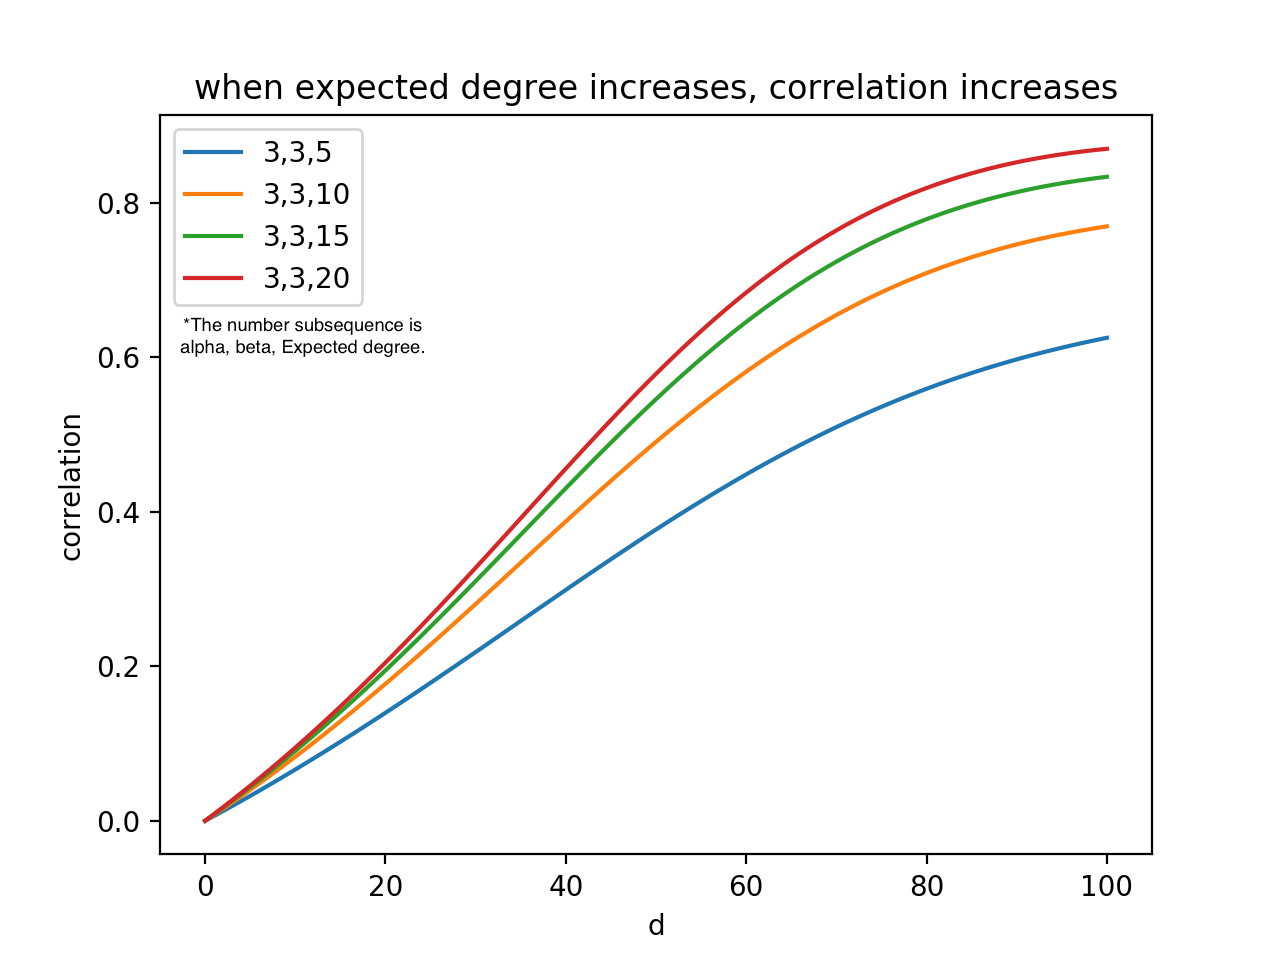
\includegraphics[width=8cm]{final_images/expected_degree.png}}
\hfill
\subfigure[Alpha]{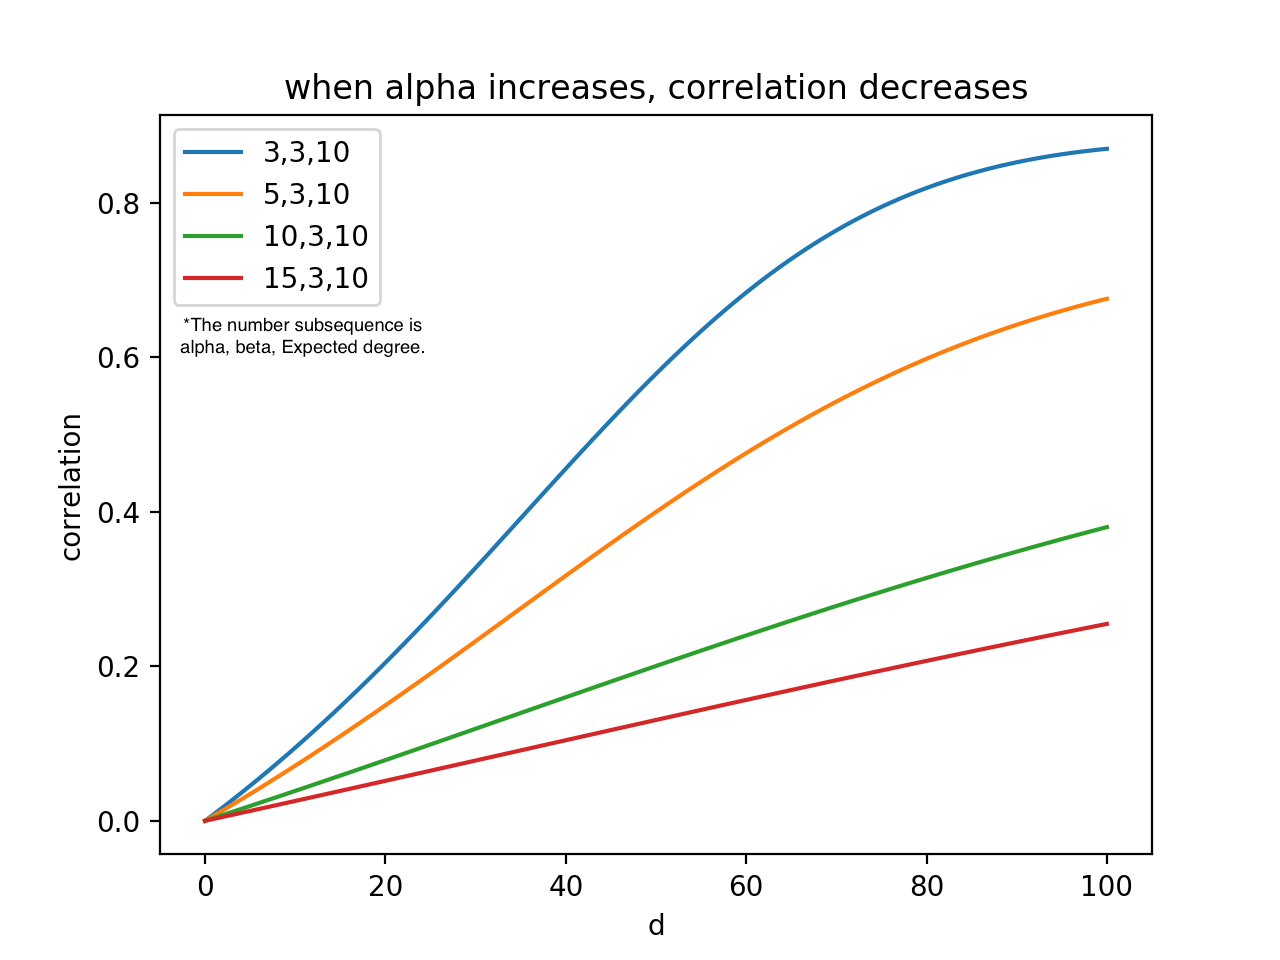
\includegraphics[width=8cm]{final_images/alpha.png}}
\hfill
\subfigure[Beta]{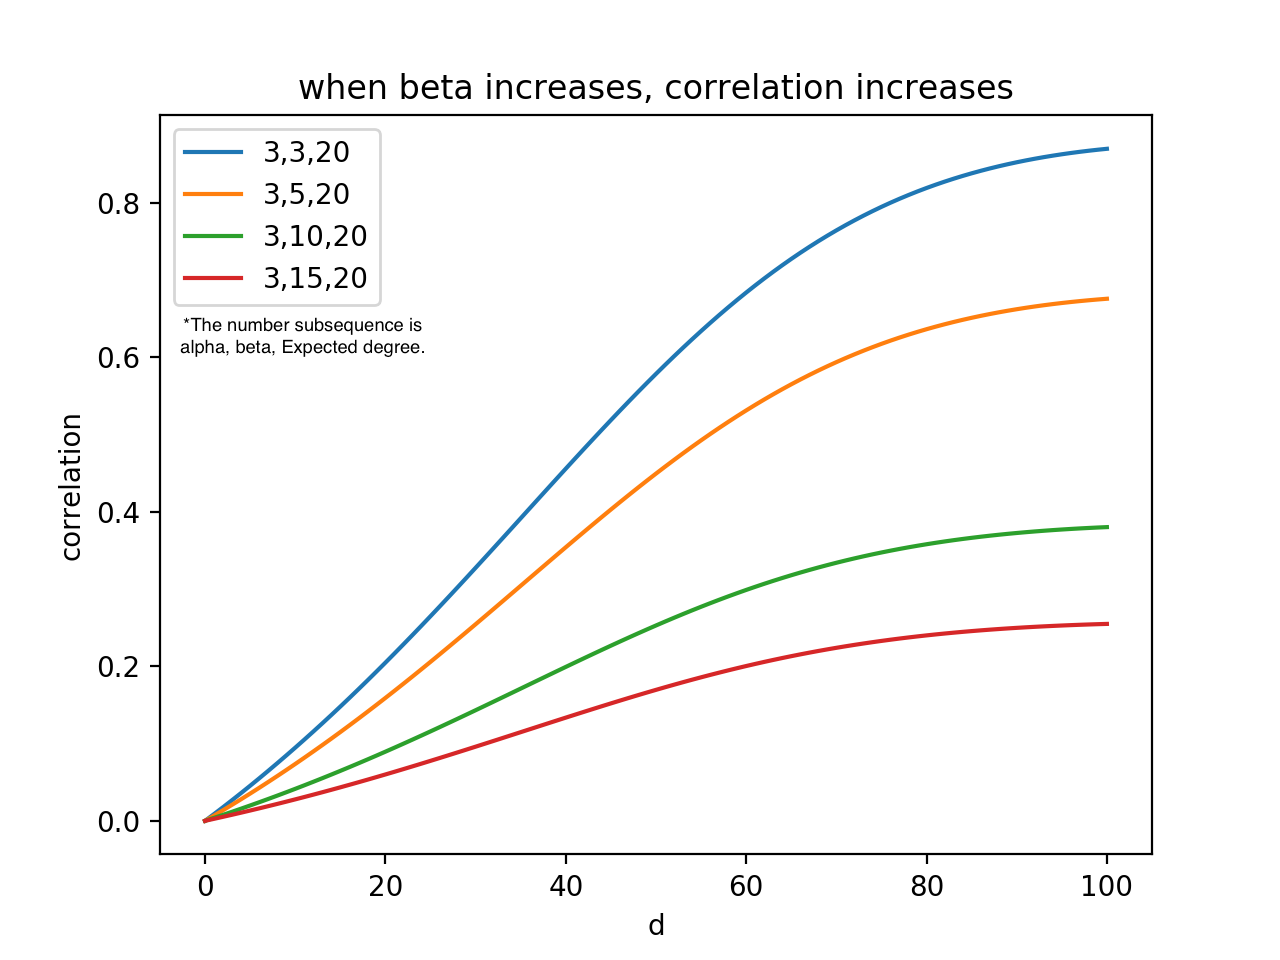
\includegraphics[width=8cm]{final_images/beta.png}}
\hfill
\caption{
\label{fig1}%
Parameters affecting degree correlation}
\end{figure}

According to Figure \ref{fig1}, we could see as $\alpha, \beta, d$ or expected degree increases independently, the degree correlation increases.


\end{itemize}

 
\end{itemize}

\subsubsection{Model Generation}
\par We denote $E$ the expected degree of nodes, and $n$  the graph size, that is, the total number of nodes in a graph, in the following context.
\par In DCM generation, we only need to fix the value of $\alpha, \beta, d, E,$ and $n$ to determine the model.

\begin{enumerate}
\item Degree Sequence Generation \\
Let  $P(W^- > x) = 1-(\frac{x}{c})^{- \beta}$, thus the CDF of  $W^-$ is
$$z=F(x) =1-P(W^->x)=1-(\frac{x}{c})^{-\beta}$$
The inverse function is
$$ x=F^{-1}(z)=c(1-z)^{-\frac{1}{\beta}}$$
So the steps are:

\begin{steps}
\item Generate $W^-$ by
$$U \sim \text{Uniform}(0, 1), W^{-1}=F^{-1}(U)=c(1-U)^{-\frac{1}{\beta}}$$
\item Create an independent copy of $W^-$. Note $\hat{W}^-$
\item Generate $W^+$ by
$$W^+ = ad(W^-)^S+a(1-d)(W^-)^s$$
\item Independently generate $(D^+, D^-) = (Poisson(W^+), Poisson(W^-))$.
\item Apply the sequence-modificaiton algorithm in \cite{algo} (a brief description in \hyperlink{equal_sum_algo}{sequence-modification algorithm in Appendix} ) to make the sum of in-degree sequence equal to the sum of out-degree sequence.
\end{steps}  
\item DCM generation (with Erased algorithm)
\begin{lstlisting}
import networkx as nx
 
 # generate the multigraph
 dcm = nx.directed_configuration_model(self.d_in, self.d_out)

 # remove parallel edges
 dcm = nx.DiGraph(dcm)
            
 # remove self-loops
 dcm.remove_edges_from(dcm.selfloop_edges())
\end{lstlisting}

\end{enumerate} 
\subsection{Real World Graph}
We use \emph{Wikipedia vote network} in the following tests. \\
\hypertarget{wikivote_intro}{Here is a brief introduction to \text{Wiki-Vote network}:}
`Wikipedia vote network is a directed graph reflecting the administrator election vote in the Wikipedia community. The graph data is derived from Stanford Large Network Dataset Collection. A small part of Wikipedia contributors are administrators, who are users with access to additional technical features that aid in maintenance. In order for a user to become an administrator a Request for adminship (RfA) is issued and the Wikipedia community via a public discussion or a vote decides who to promote to adminship. The network contains all the Wikipedia voting data from the inception of Wikipedia till January 2008. Nodes in the network represent wikipedia users and a directed edge from node i to node j represents that user i voted on user j.'\\
A full description and network data is in \cite{wikivote_source}


\section{Part 1: Relationship between Page Rank and Betweeness Centrality}
\par In this part, we want to find out the relationship between page rank and betweenness centrality, especially how it changes as the degree correlation changes.\par Fixing the values of power-law index ($\alpha$ and $\beta$), we adjust the value of d from 0 to 1 to vary the degree correlation, and then observe how the relationship between page rank and betweenness centrality changes.
\subsection{Method Description}
In this part we introduce two measures of correlation between PageRank and Betweeness centrality.
\subsubsection{Statistical approach: Spearman's Rank Correlation }
\par `In statistics, a rank correlation is any of several statistics that measure an ordinal association—the relationship between rankings of different ordinal variables or different rankings of the same variable, where a "ranking" is the assignment of the labels "first", "second", "third", etc. to different observations of a particular variable. A rank correlation coefficient measures the degree of similarity between two rankings, and can be used to assess the significance of the relation between them.' \cite{spearman} 
\par We use Spearsman's test to measure the rank correlation between page rank and betweenness centrality.

\subsubsection{Visual approach: Ranking Plot}
\par Make a scatterplot of Page Rank and Betweenness centrality of top k nodes in decreasing order of Page Rank or Betweenness centrality. We would expect to see an absolute dowward curve, and conclude that if the other scatter plot is less scattered and more downward-habaved, the correlation between Page Rank and Betweenness Centrality is more obvious.

\subsection{Experiment and Analysis}
\par In this part, we fix the values of $\alpha, \beta$ and expected degree and vary the value of d from 0 to 1 to change the degree correlation, and observe how rank correlation changes. Since spearman's correlation between PR and BC is a random variable, for each model we repeat the simulation for 20 times independently to obtain the sample correlation between PR and BC.

\subsubsection{Case1: $\alpha=\beta$}
\par In the simulation, fix $\alpha=\beta=3, E=20, n=5000$ and let $d$ vary from 0 to 1 with step size 0.2, to make the degree correlation vary from 0 to 0.943. The simulation results are given in \ref{table1}, \ref{fig: corrs_1}.and the detailed information of the models are given in excel files (TODO: attach github link).

\begin{enumerate}
\item Ranking Plot \\
From Figure \ref{case1rankplotPR}, we plot PageRank and Betweenness Centrality values of the top 200 nodes in decreasing order of Page Rank, so that the PageRank plot (red color) must be a downward curve. We could see that as $d$ increases (thereby degree correlation increases), dots identifying Betweenness Centrality  become less scattered, and behave more like a downward trend as does Page Rank curve. We could observe a similar trend in Figure \ref{case1rankplotBC} as well.

\begin{figure}[!hbtp]
\hfill
\subfigure[d=0]{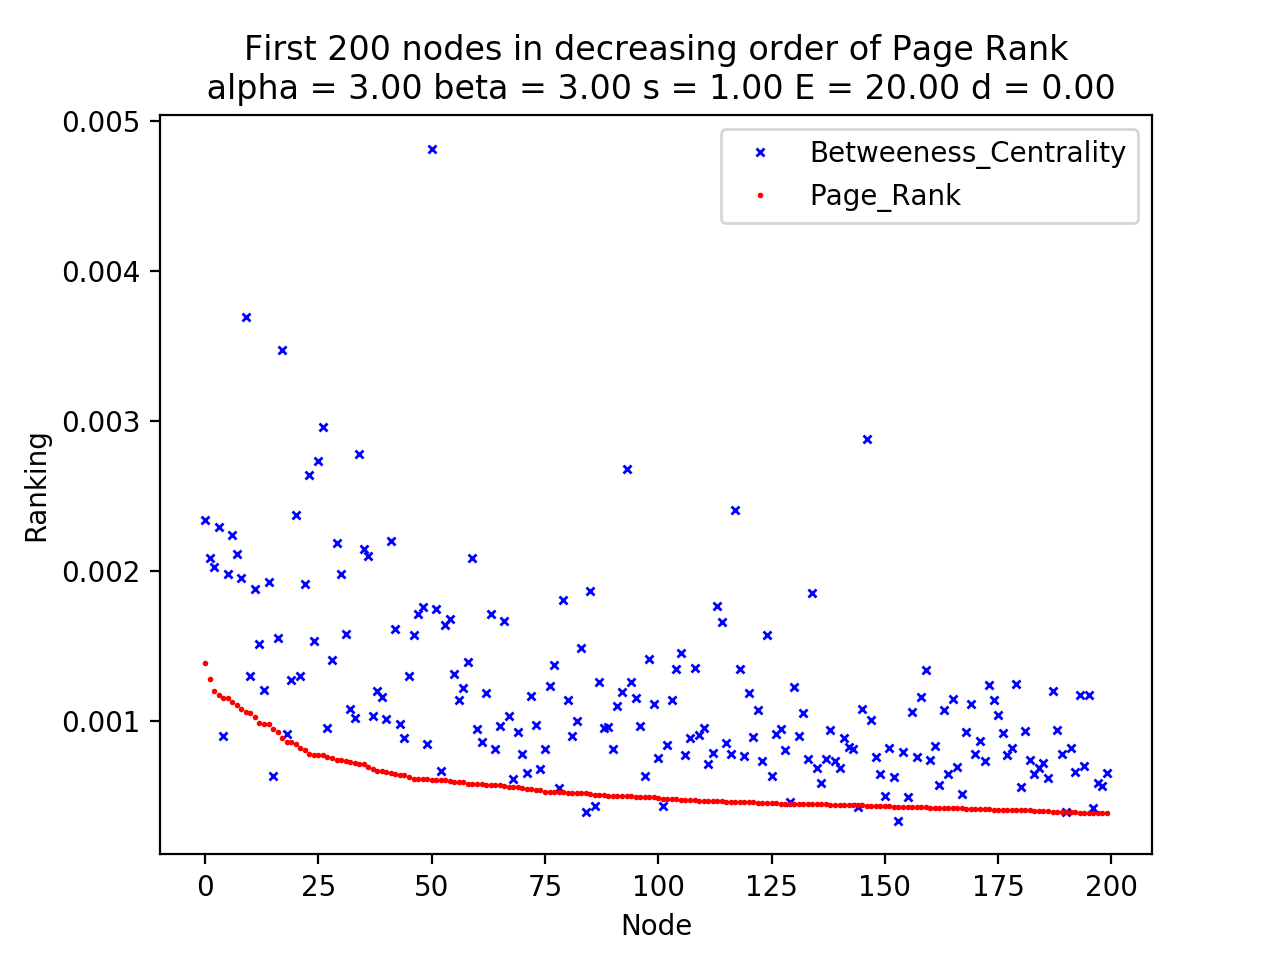
\includegraphics[width=8cm]{final_images/m1_prbc.png}}
\hfill
\subfigure[d=0.2]{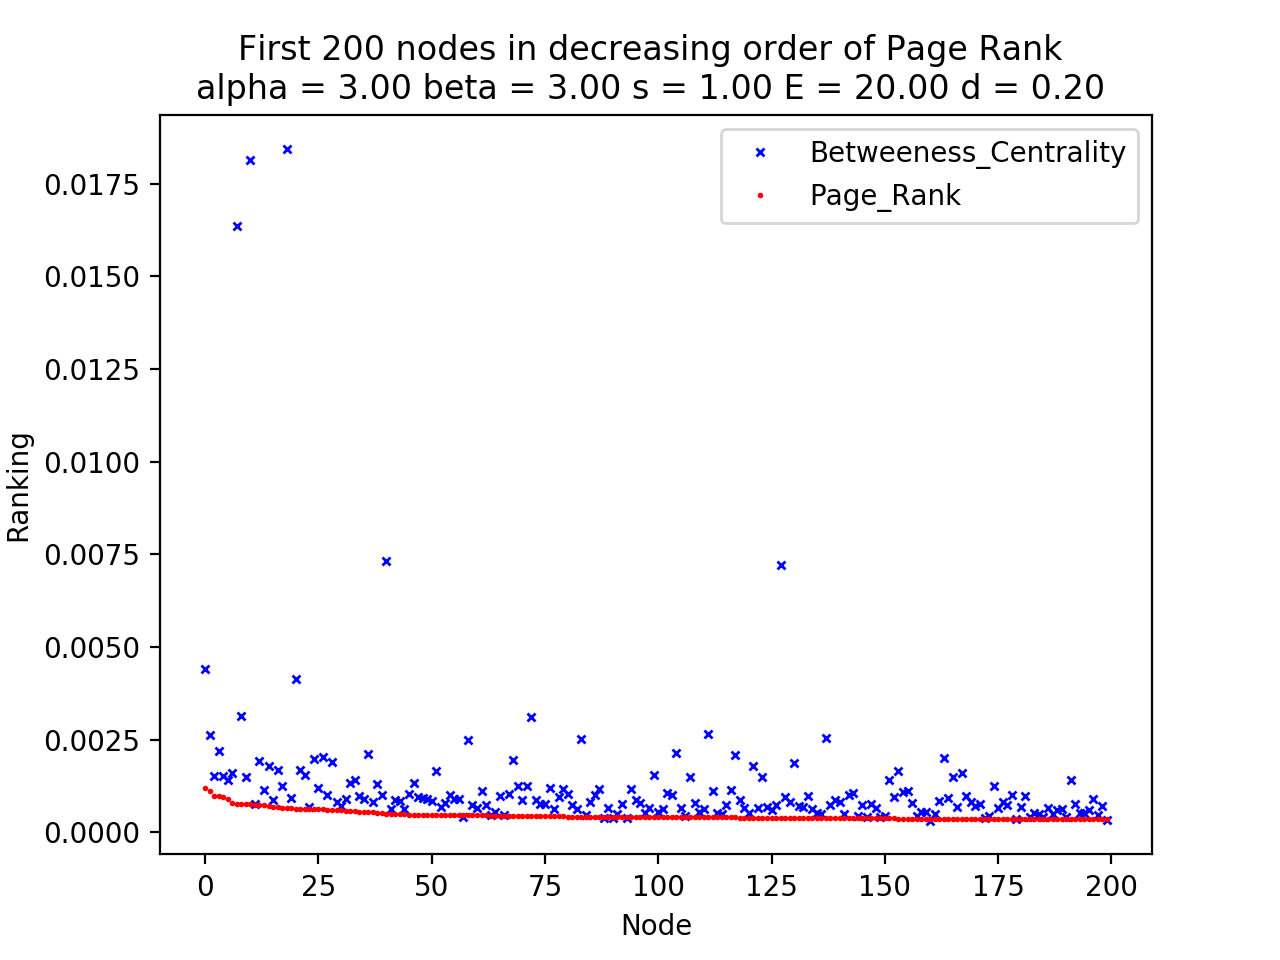
\includegraphics[width=8cm]{final_images/m2_prbc.png}}
\hfill
\subfigure[d=0.4]{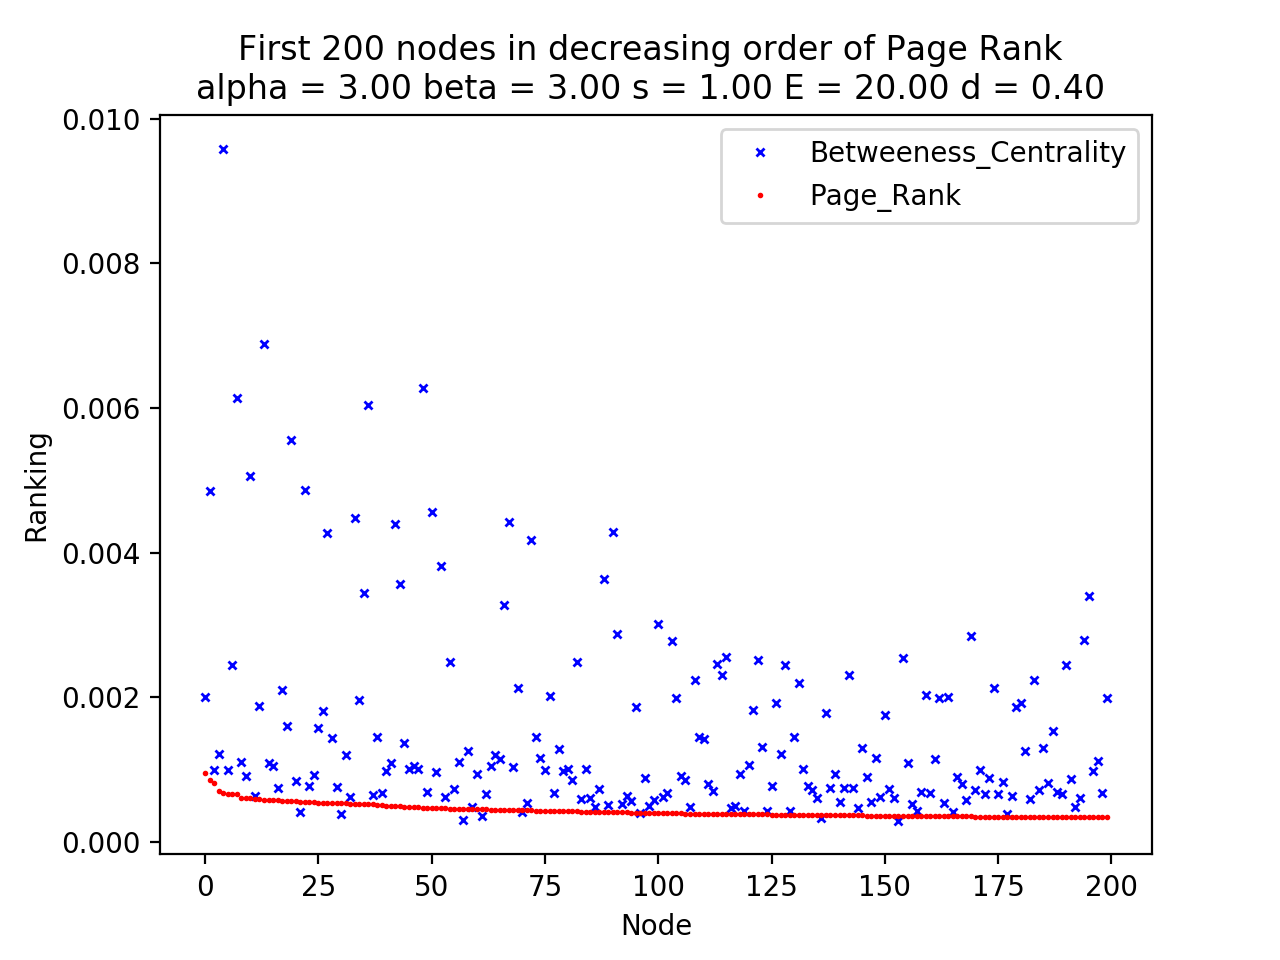
\includegraphics[width=8cm]{final_images/m3_prbc.png}}
\hfill
\subfigure[d=0.6]{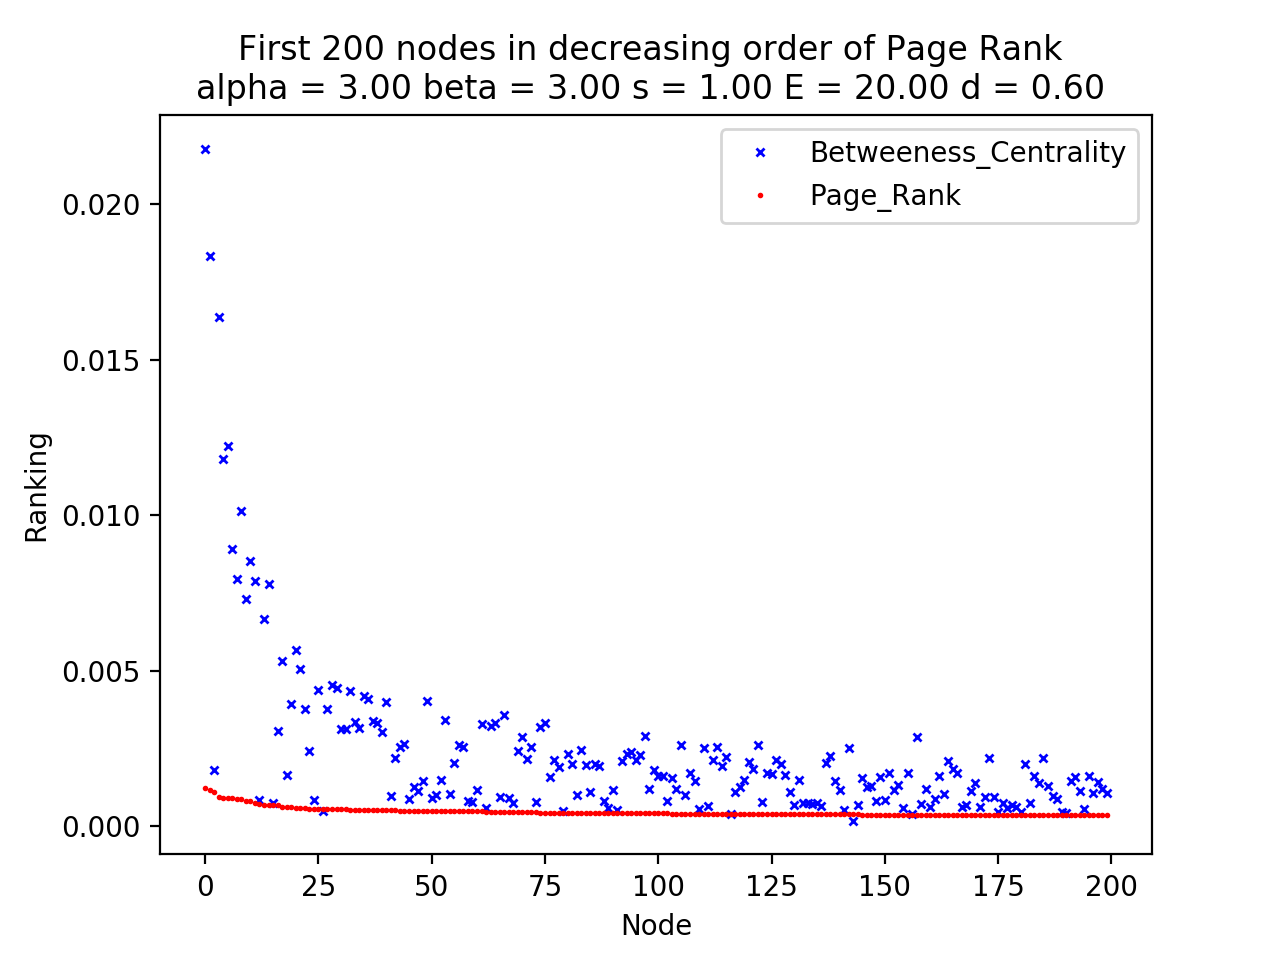
\includegraphics[width=8cm]{final_images/m4_prbc.png}}
\hfill
\subfigure[d=0.8]{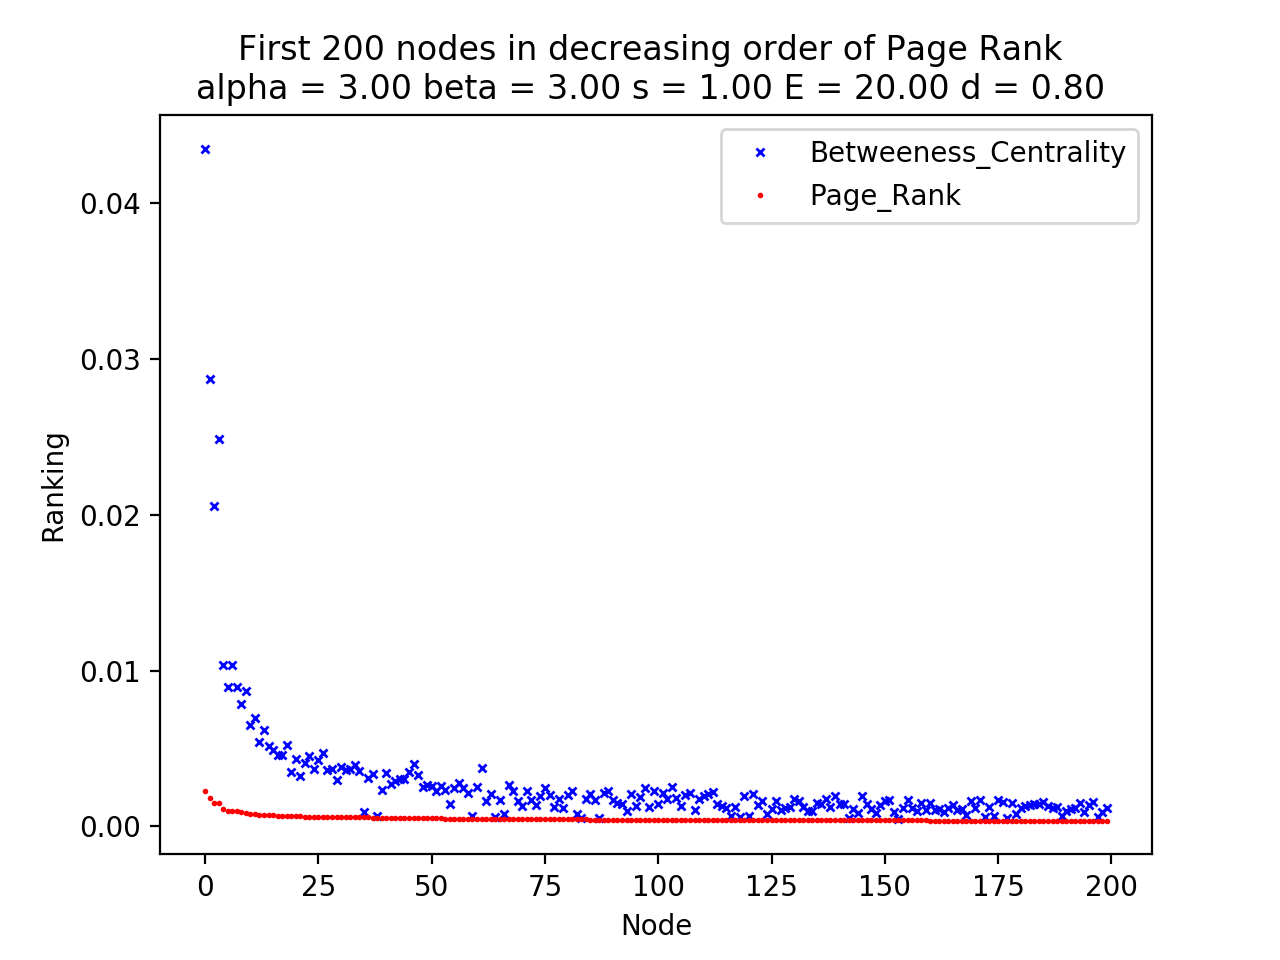
\includegraphics[width=8cm]{final_images/m5_prbc.png}}
\hfill
\subfigure[d=1.0]{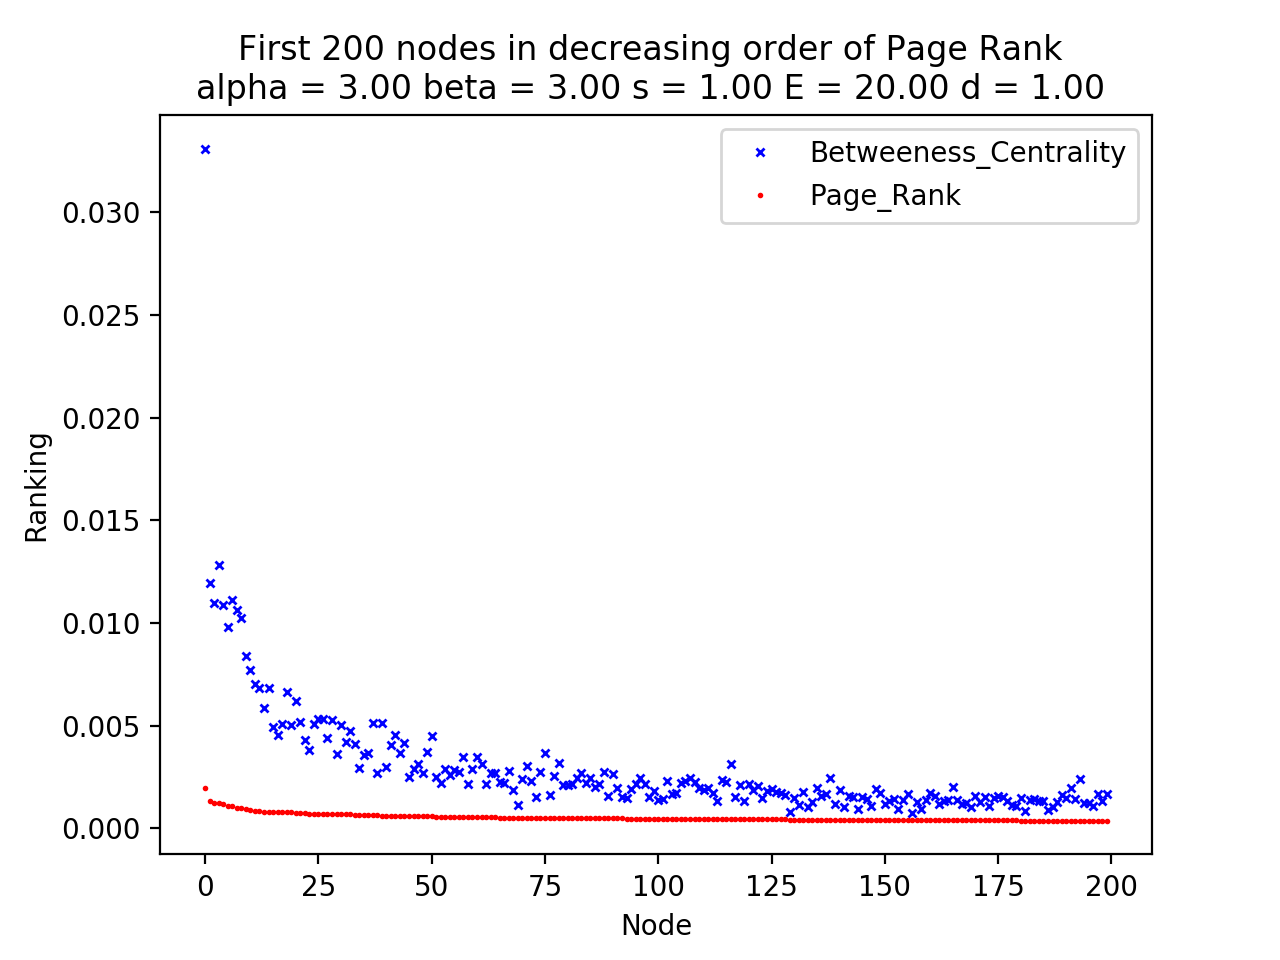
\includegraphics[width=8cm]{final_images/m6_prbc.png}}
\hfill
\caption{
\label{case1rankplotPR}%
Page Rank and Betweeness Centrality values of First 200 nodes in decreasing order of Page Rank}
\end{figure}

\begin{figure}[!hbtp]
\hfill
\subfigure[d=0]{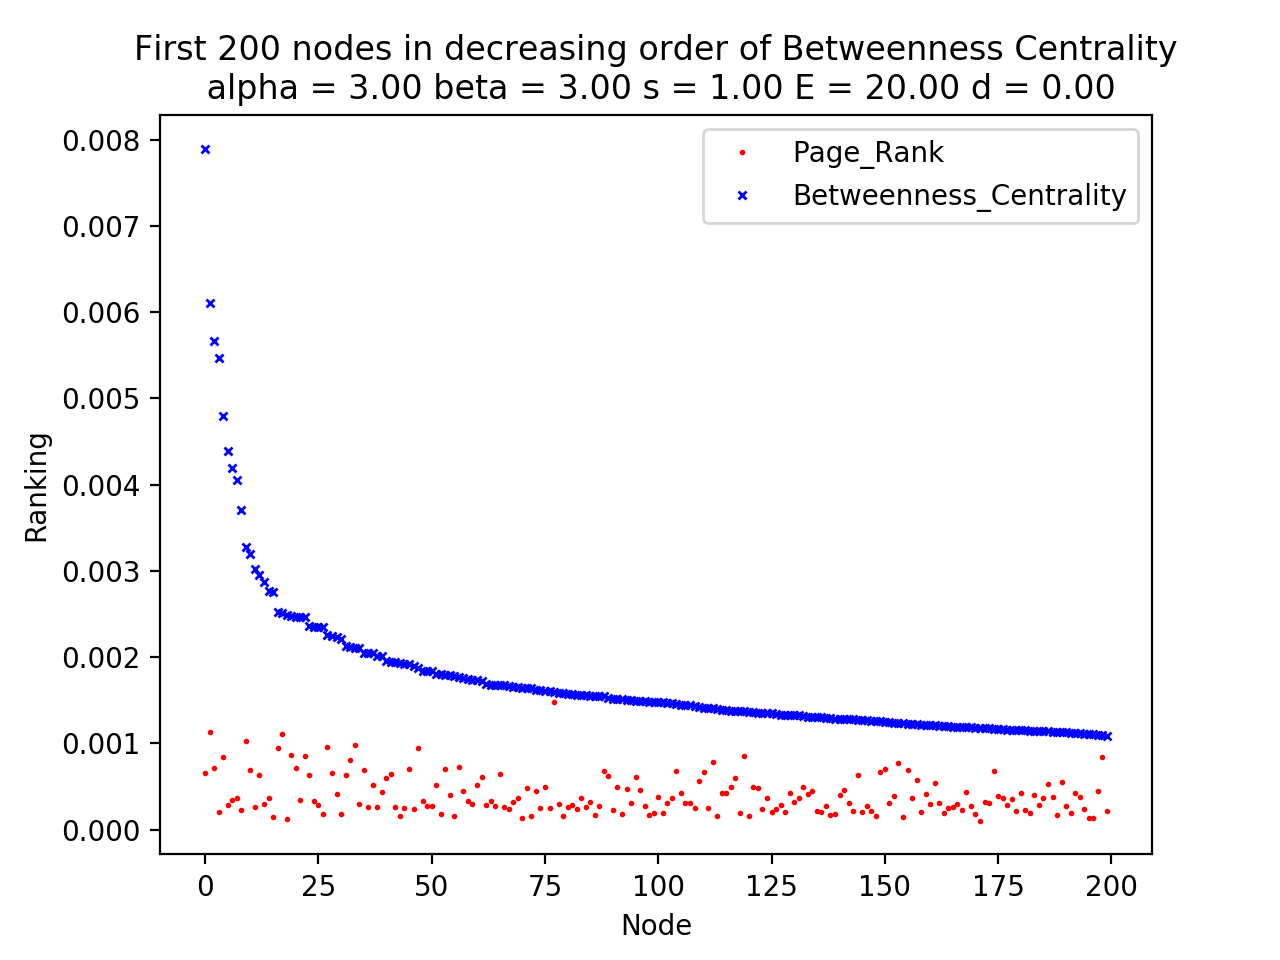
\includegraphics[width=8cm]{final_images/m1_bcpr.png}}
\hfill
\subfigure[d=0.2]{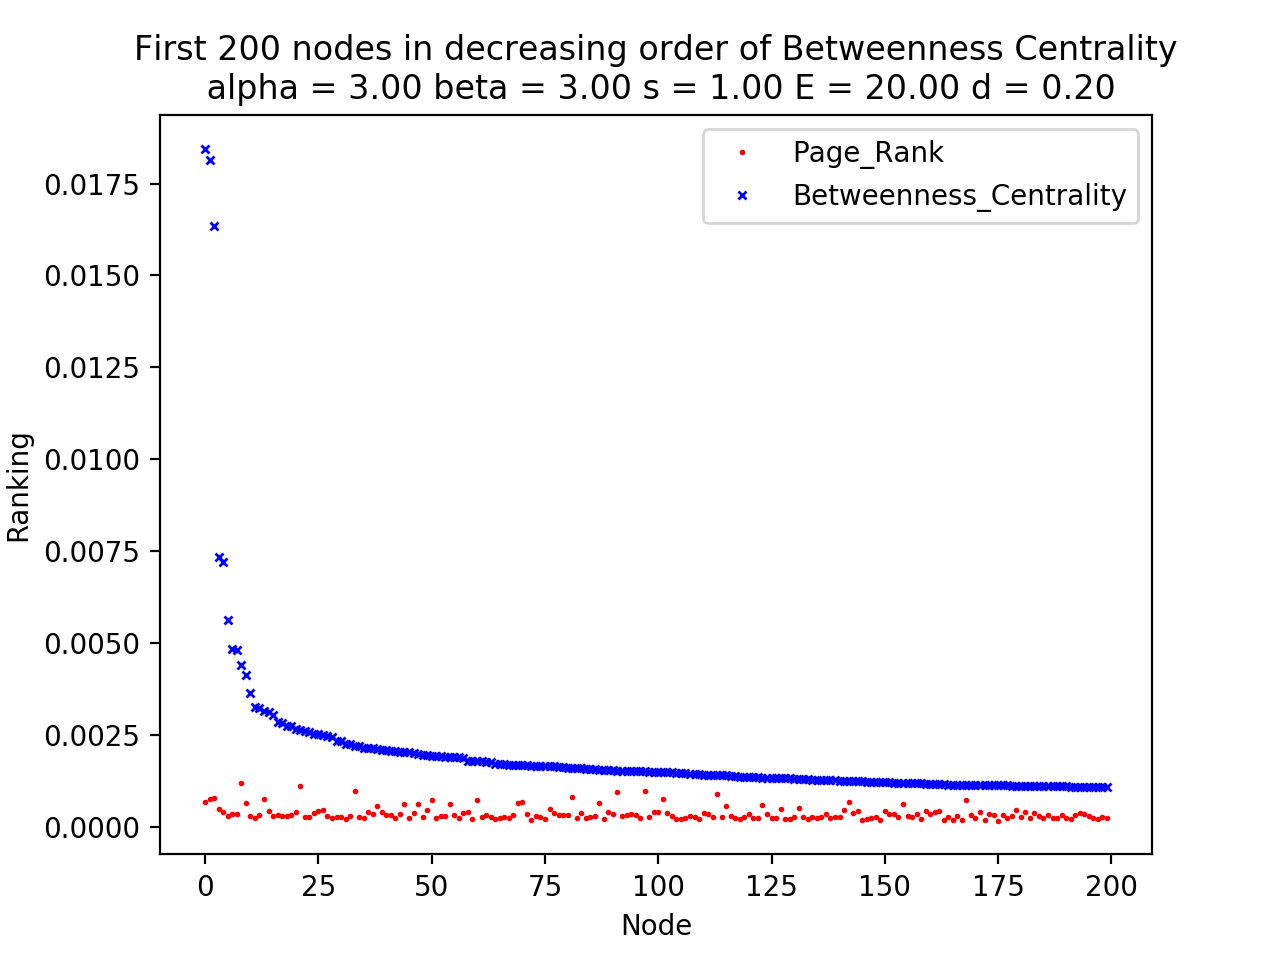
\includegraphics[width=8cm]{final_images/m2_bcpr.png}}
\hfill
\subfigure[d=0.4]{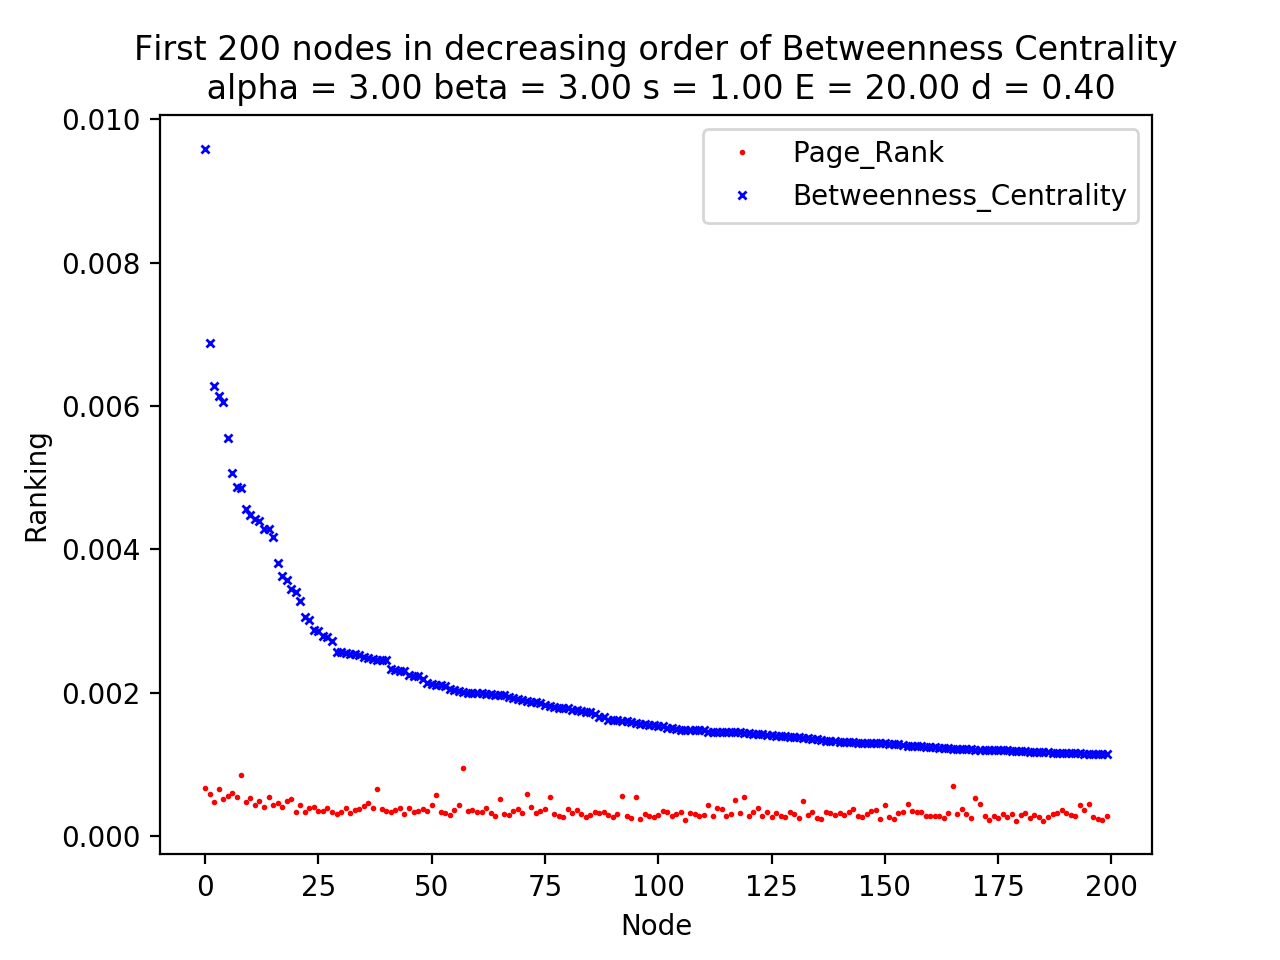
\includegraphics[width=8cm]{final_images/m3_bcpr.png}}
\hfill
\subfigure[d=0.6]{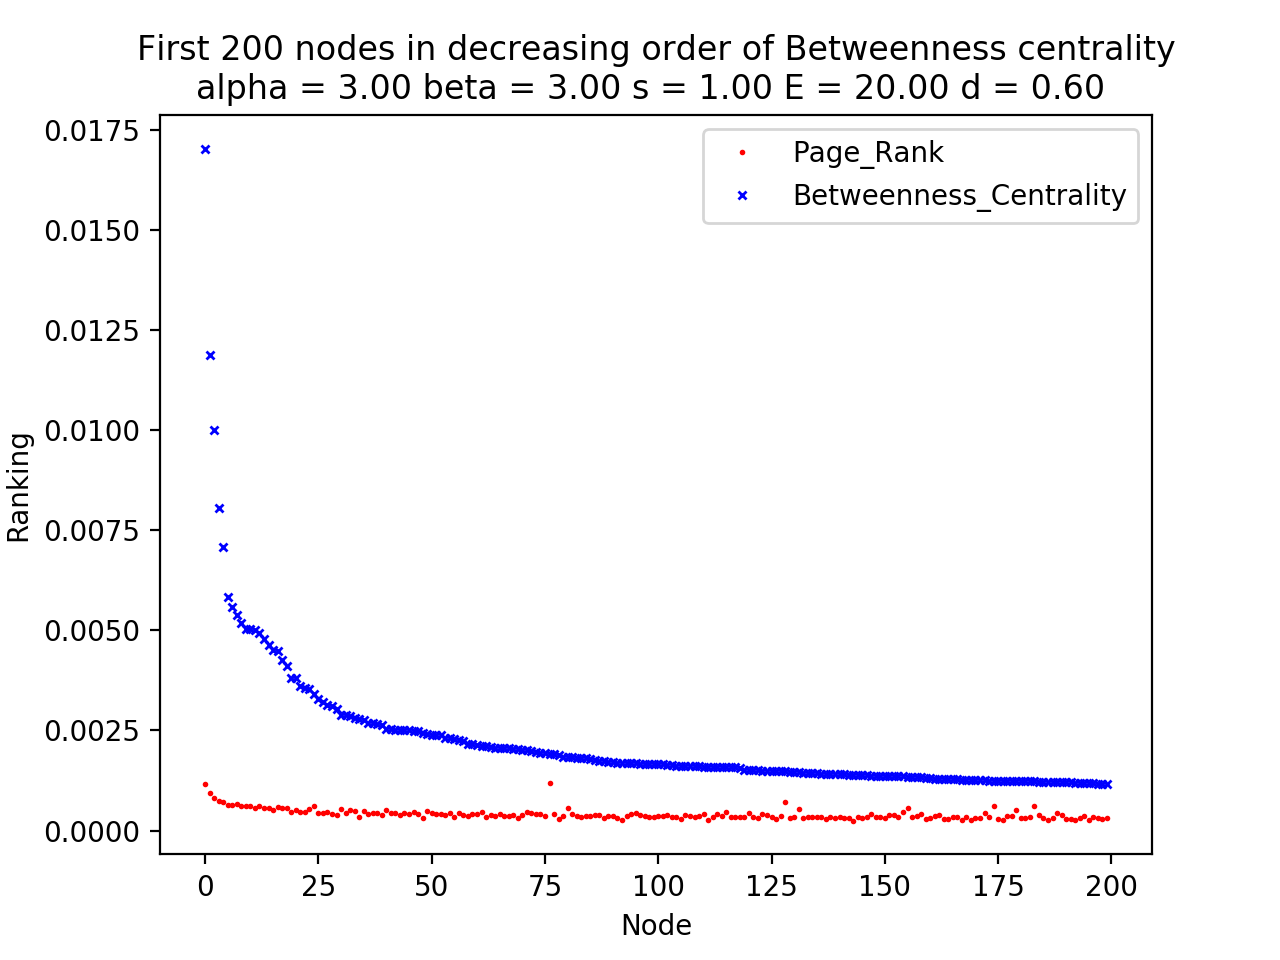
\includegraphics[width=8cm]{final_images/m4_bcpr.png}}
\hfill
\subfigure[d=0.8]{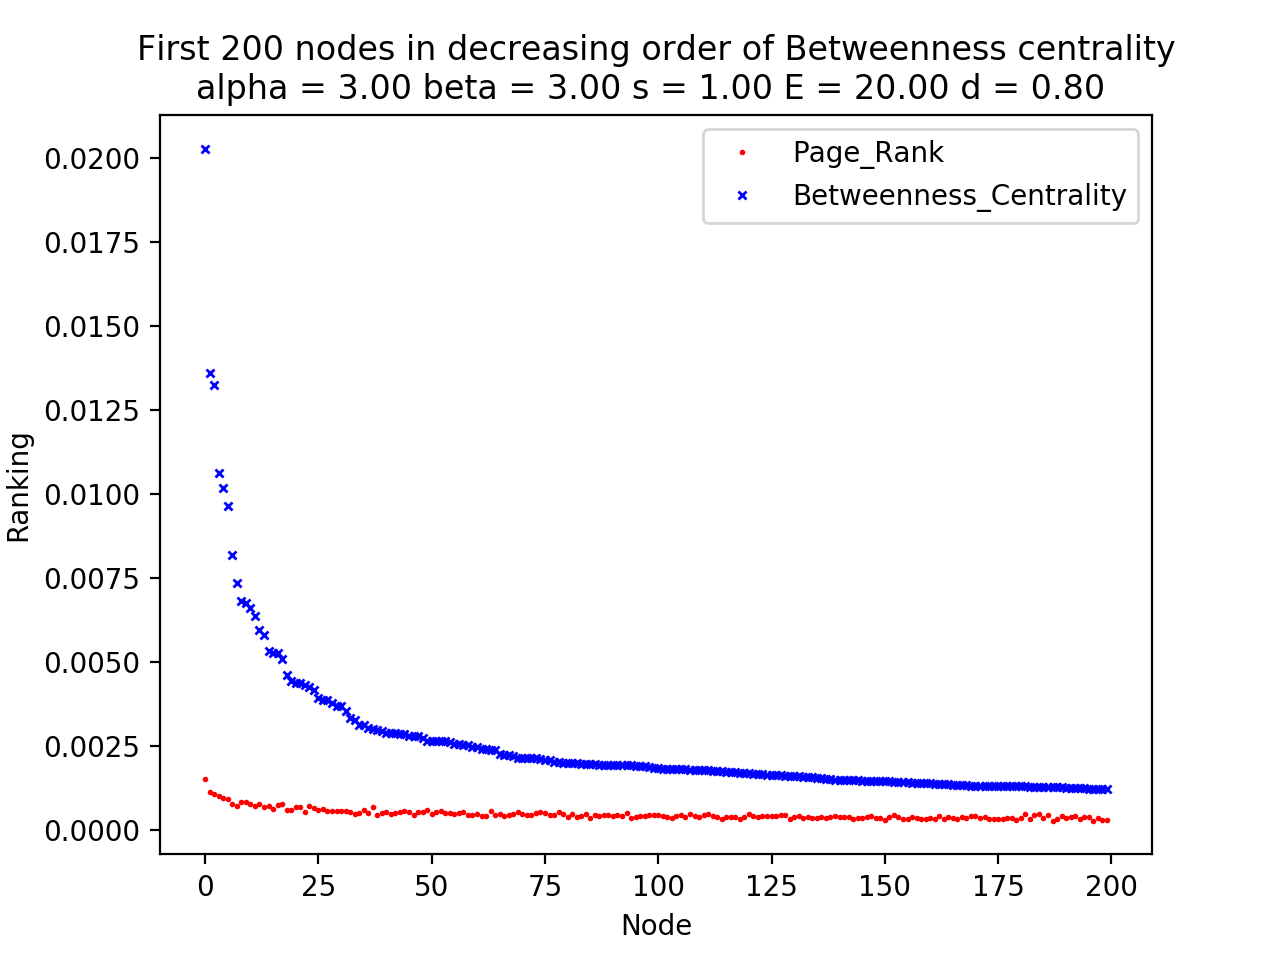
\includegraphics[width=8cm]{final_images/m5_bcpr.png}}
\hfill
\subfigure[d=1.0]{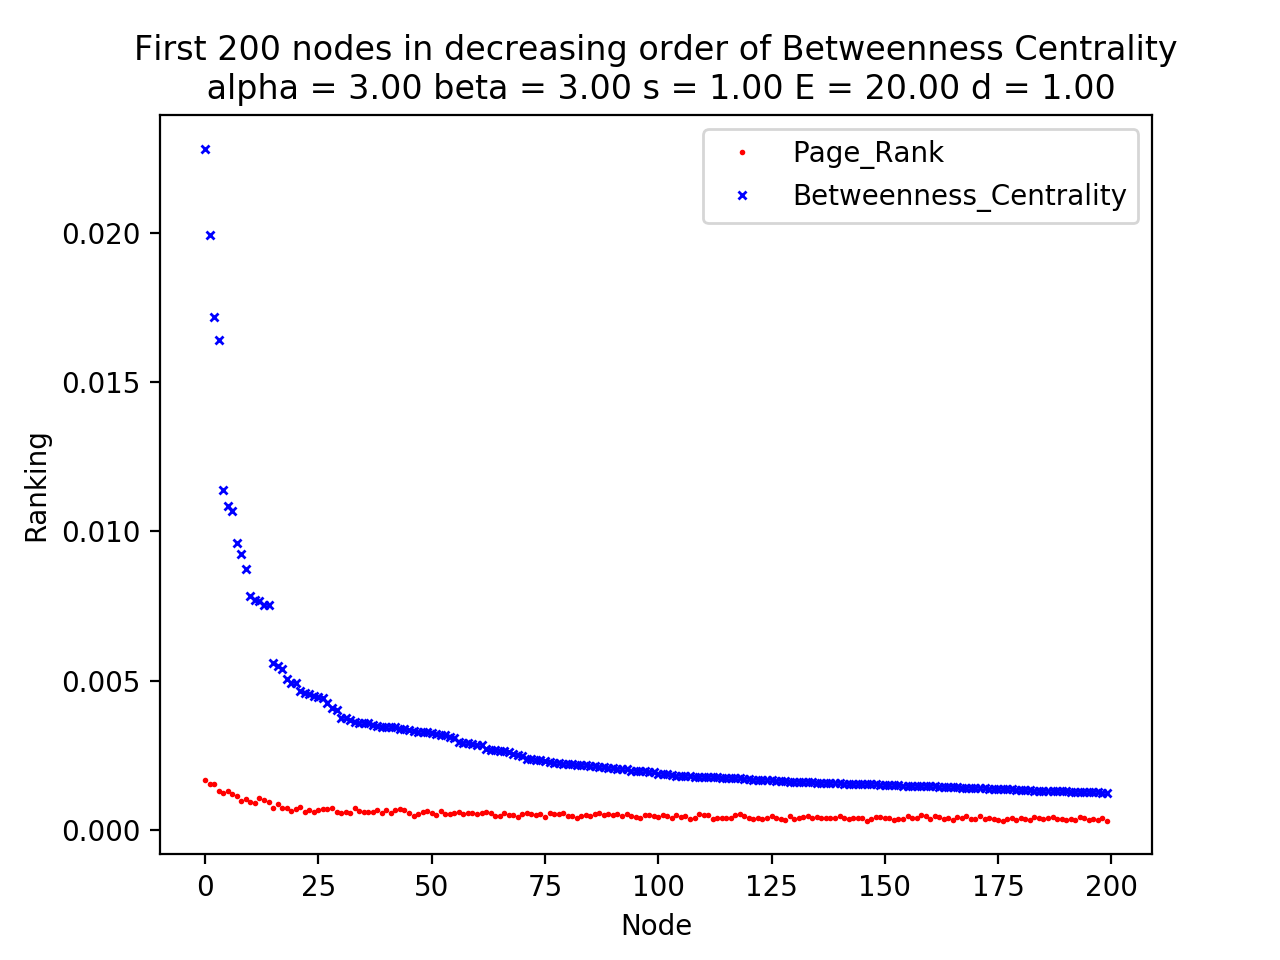
\includegraphics[width=8cm]{final_images/m6_bcpr.png}}
\hfill
\caption{
\label{case1rankplotBC}%
Page Rank and Betweenness Centrality values of First 200 nodes in decreasing order of Betweenness Centrality}
\end{figure}


\item Rank Correlation
\begin{enumerate}

\item From Table \ref{table1}, we could see that the sample variance of rank correlation is close to 0, which suggests that the sample average of rank correlation is representative.
\item From Figure \ref{fig: corrs_1}, we could see as d increases,  degree correlation increases, and rank correlation increases.
\begin{table}[]
\centering
\caption{Case1 ($\alpha=\beta$): statistics of rank correlation over 20 samples}
\label{table1}
\begin{tabular}{|l|l|l|l|}
\hline
d   & computed degree correlation & average of rank correlation & variance of rank correlation \\
\hline
0   & 0                           & 0.668137886                            & 7.28353E-05                         \\
\hline
0.2 & 0.2047114                   & 0.711738476                            & 5.53925E-05                         \\
\hline
0.4 & 0.455694377                 & 0.754644549                            & 4.67439E-05                         \\
\hline
0.6 & 0.683541566                 & 0.786671926                            & 0.000186392                         \\
\hline
0.8 & 0.818845602                 & 0.816479938                            & 9.33524E-05                         \\
\hline
1.0 & 0.869565217                 & 0.8455353                              & 0.000119224                        
\\
\hline
\end{tabular}
\end{table}


\begin{figure}
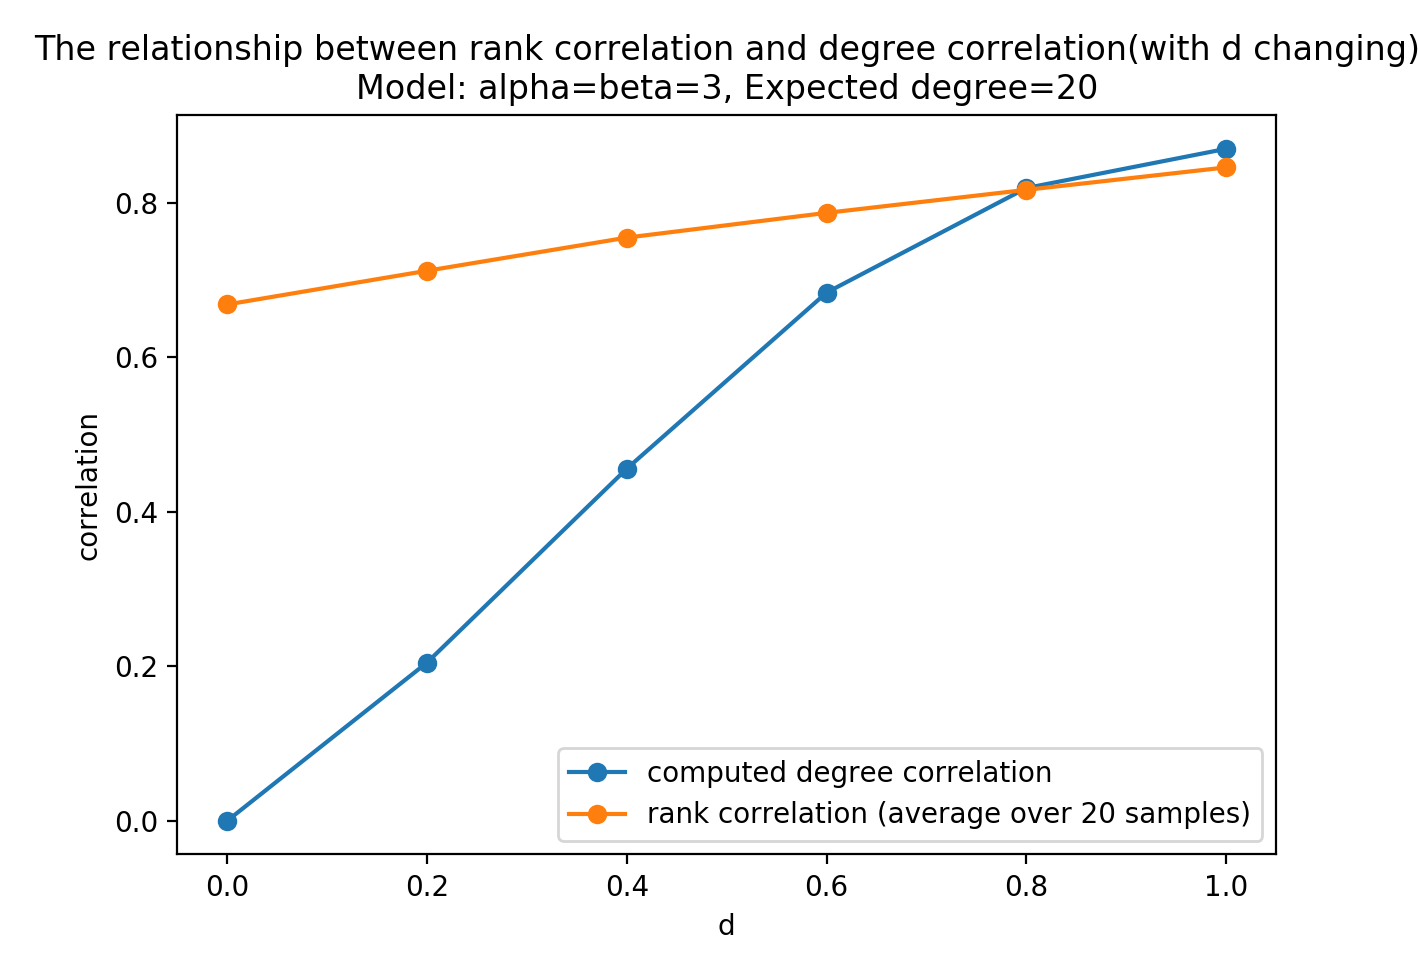
\includegraphics[scale=1]{final_images/corrs_relation.png}
\caption{Case1($\alpha=\beta$): relationship between rank correlation and degree correlation}
\label{fig: corrs_1}
\end{figure}

\end{enumerate}

\end{enumerate}

\subsubsection{Case2: $\alpha \neq \beta$}
\par In this simulation, fix $\alpha=3, \beta=5$, and expected degree $E = 50$, graph size $ n=5000$ and let d vary from 0 to 1, with step size 2,  to make the degree correlation vary from 0 to 0.816.

\begin{enumerate}
\item Ranking Plot \\
From Figure \ref{case2rankplotPR}, we plot Page Rank and Betweenness Centrality values of the top 200 nodes in decreasing order of Page Rank, so that the Page Rank plot (red color) is a downward curve. We could see that as $d$ increases (thereby degree correlation increases), scatterplot of Betweenness Centrality  becomes less scattered, and behaves more like a downward trend as does Page Rank curve. We could observe a similar trend in Figure \ref{case2rankplotBC} as well.\\

\begin{figure}[!hbtp]
\hfill
\subfigure[d=0]{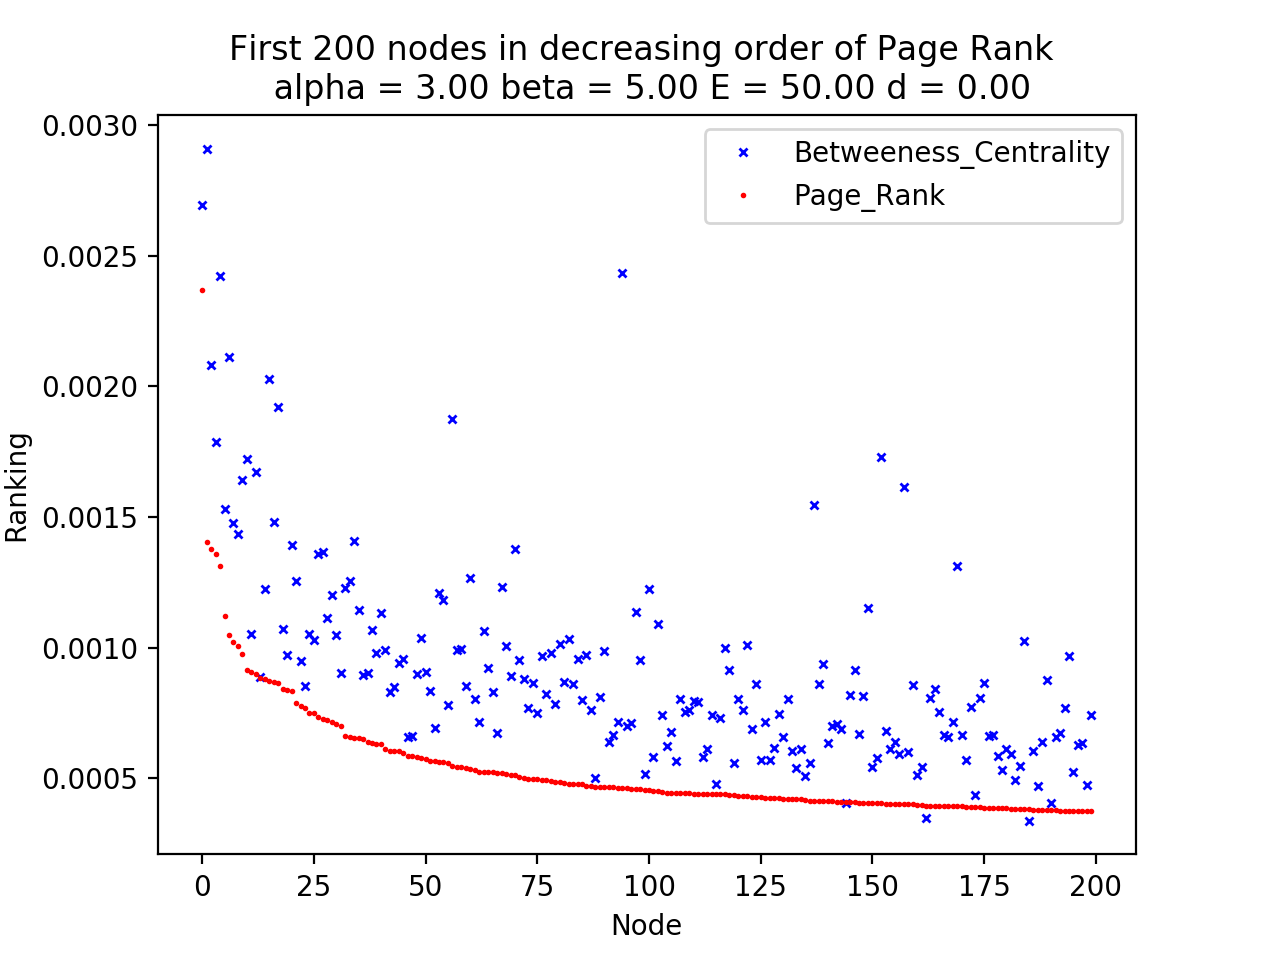
\includegraphics[width=8cm]{final_images/case2_m1_prbc.png}}
\hfill
\subfigure[d=0.2]{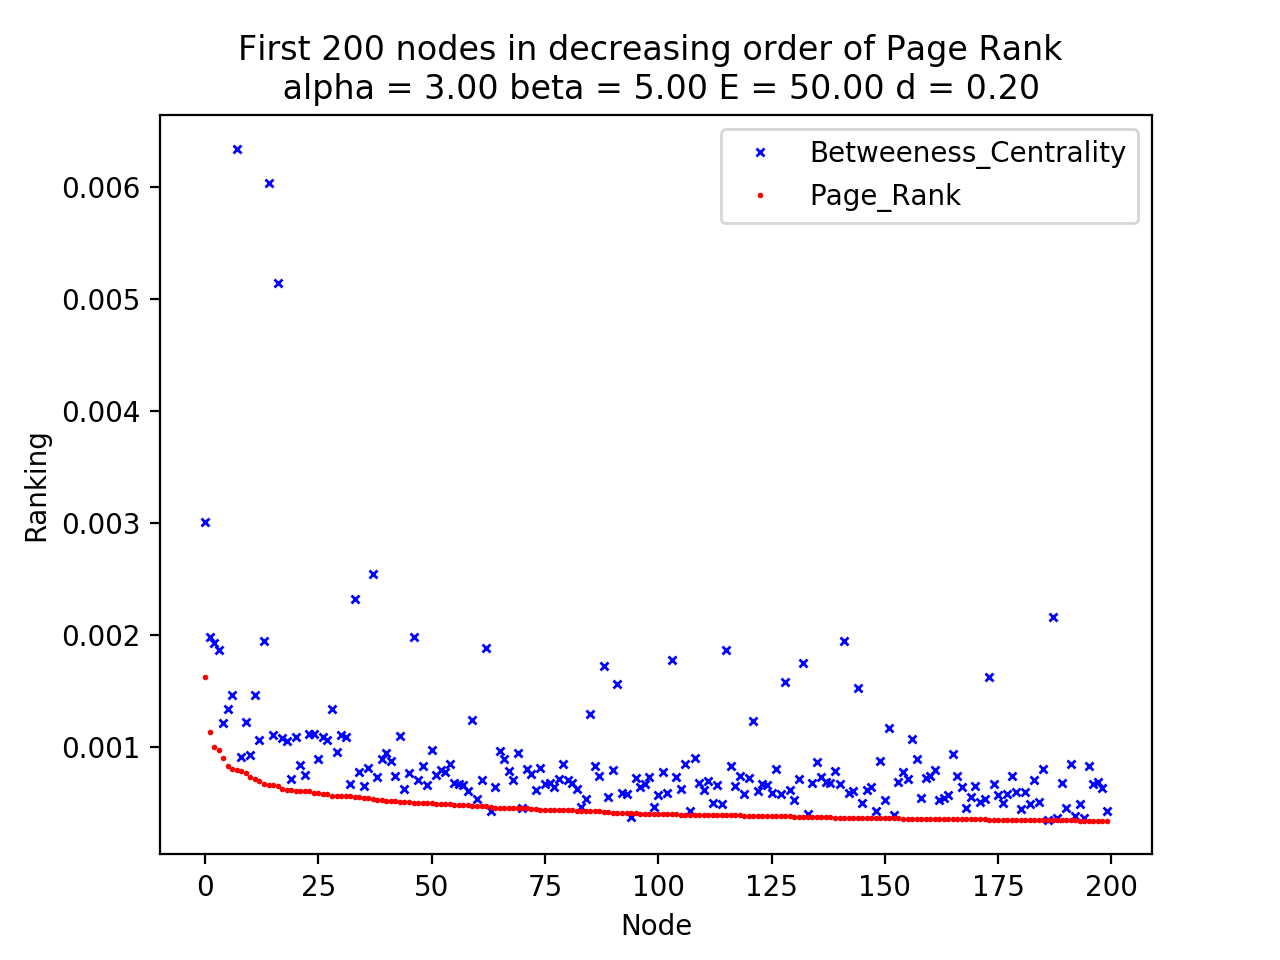
\includegraphics[width=8cm]{final_images/case2_m2_prbc.png}}
\hfill
\subfigure[d=0.4]{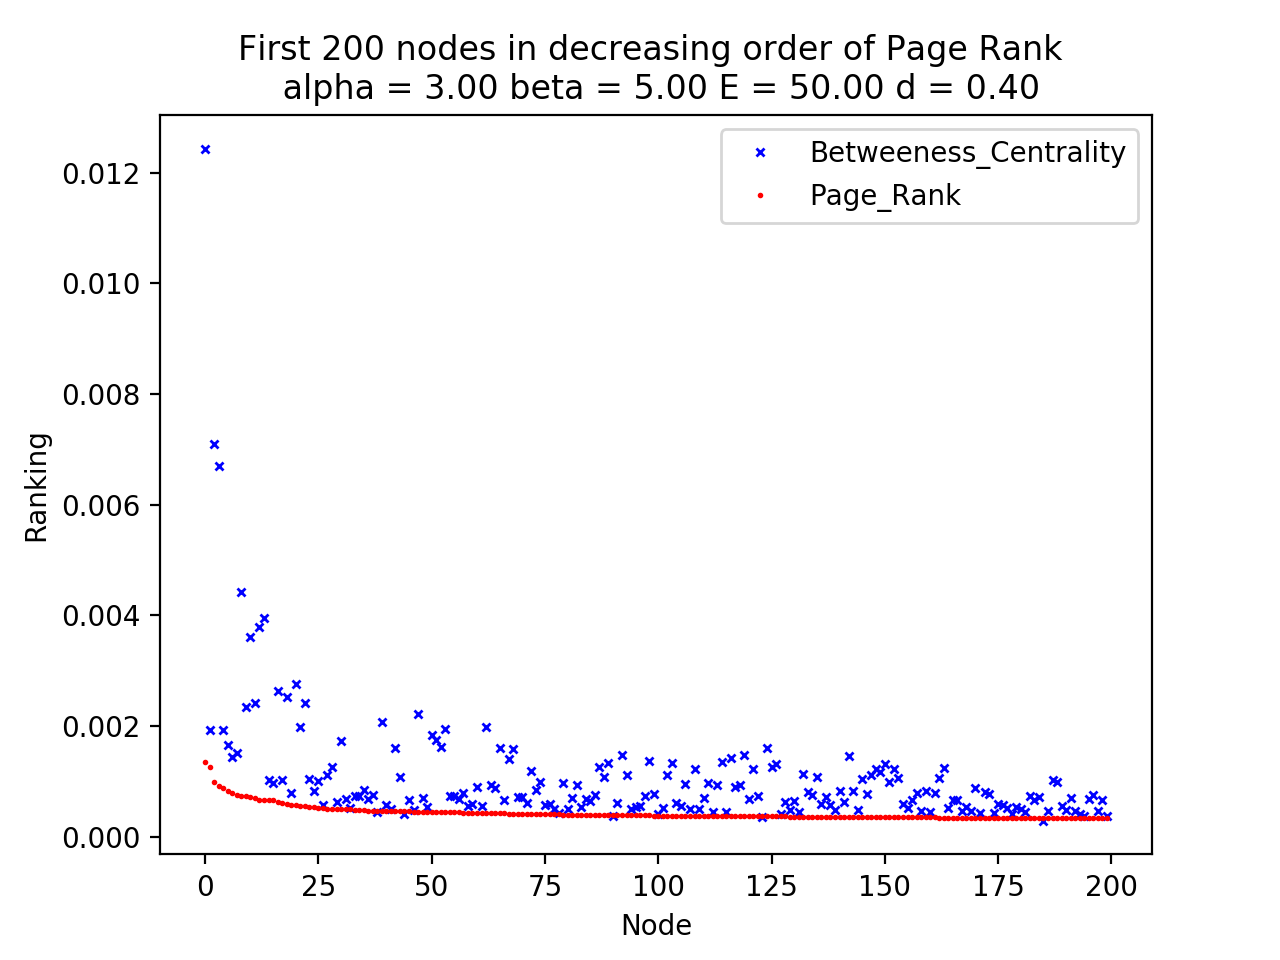
\includegraphics[width=8cm]{final_images/case2_m3_prbc.png}}
\hfill
\subfigure[d=0.6]{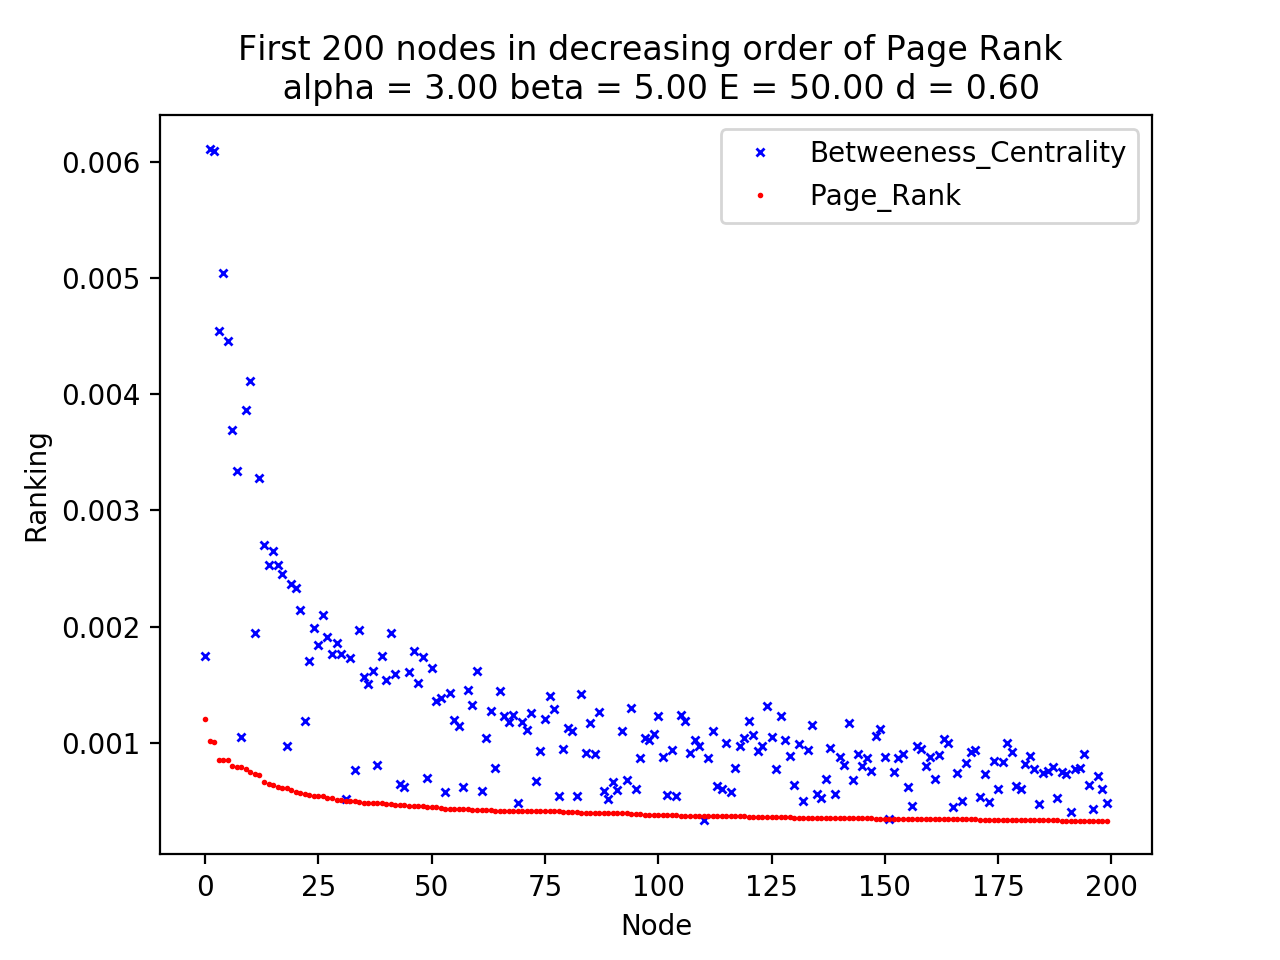
\includegraphics[width=8cm]{final_images/case2_m4_prbc.png}}
\hfill
\subfigure[d=0.8]{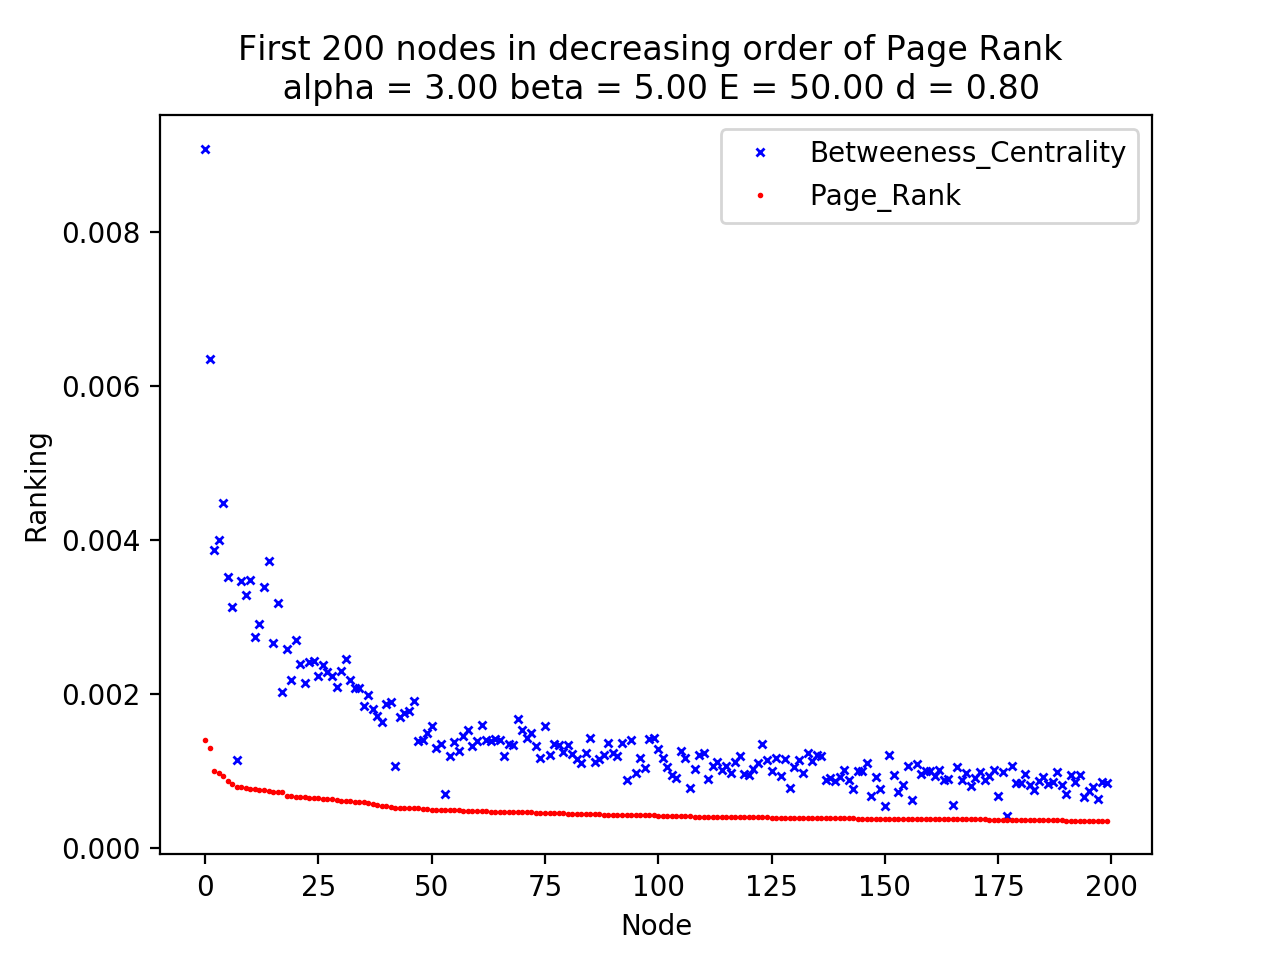
\includegraphics[width=8cm]{final_images/case2_m5_prbc.png}}
\hfill
\subfigure[d=1.0]{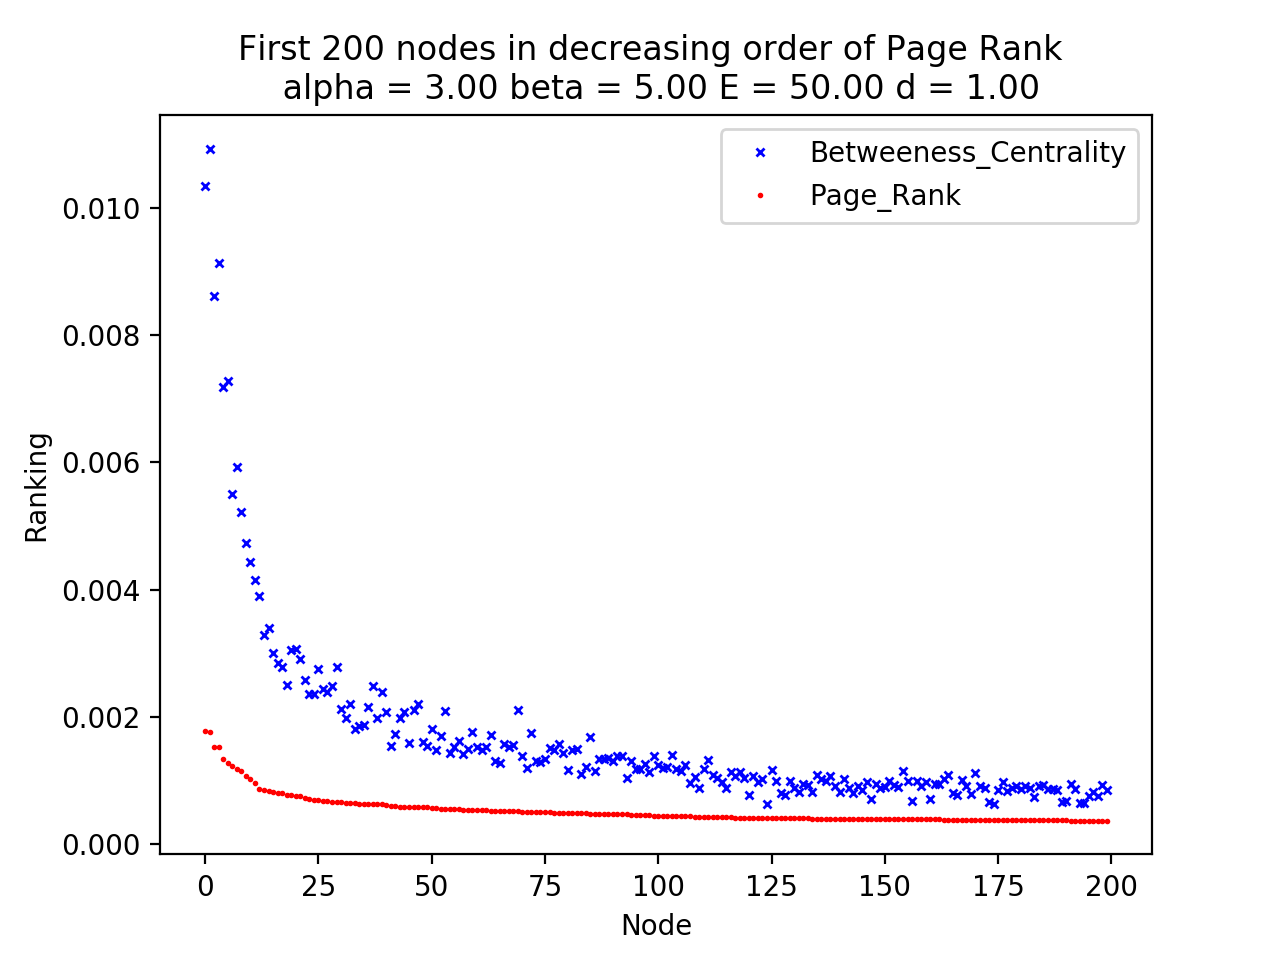
\includegraphics[width=8cm]{final_images/case2_m6_prbc.png}}
\hfill
\caption{
\label{case2rankplotPR}%
Page Rank and Betweeness Centrality values of First 200 nodes in decreasing order of Page Rank}
\end{figure}

\begin{figure}[!hbtp]
\hfill
\subfigure[d=0]{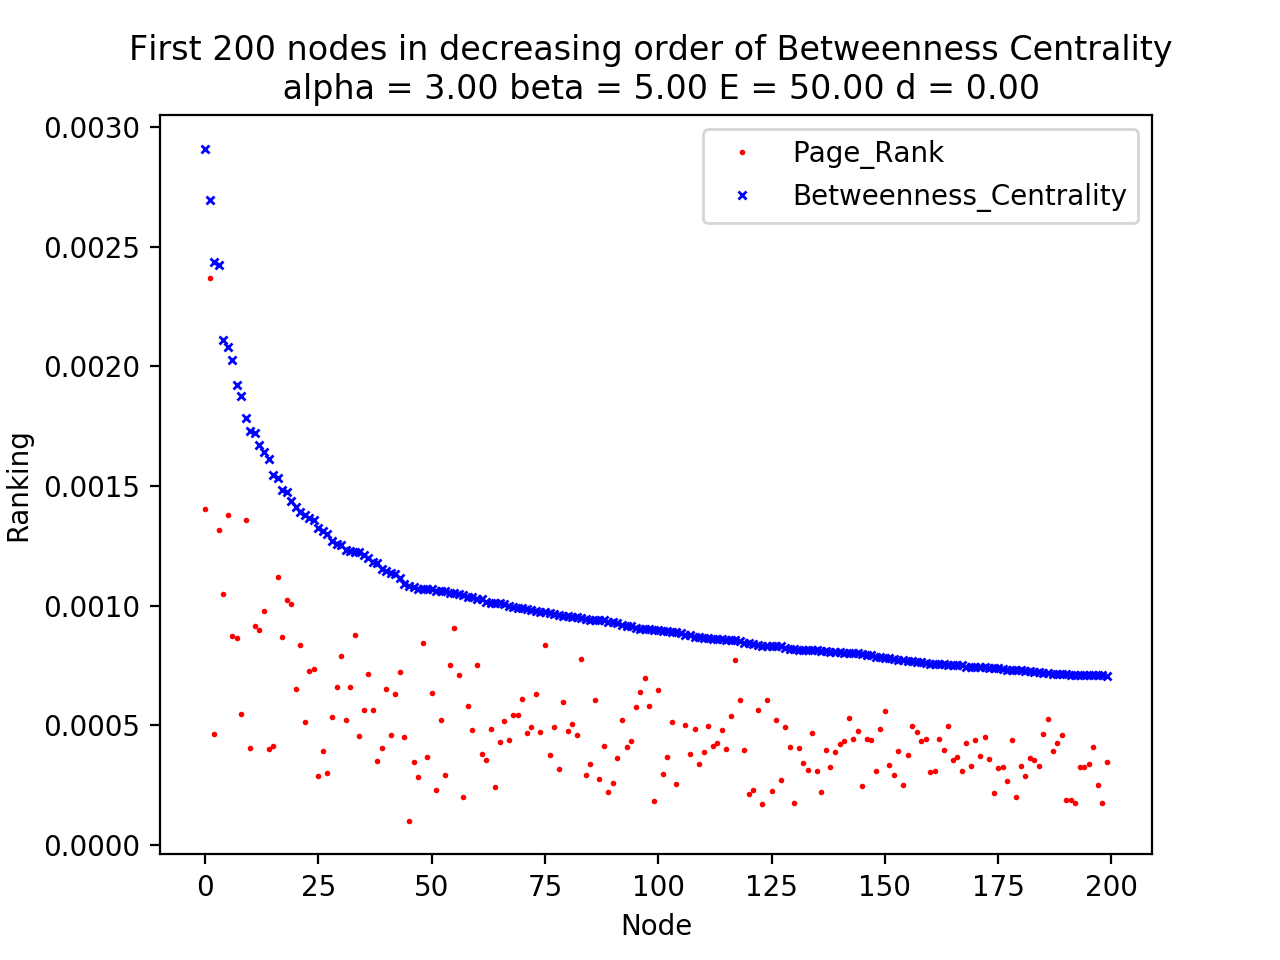
\includegraphics[width=8cm]{final_images/case2_m1_bcpr.png}}
\hfill
\subfigure[d=0.2]{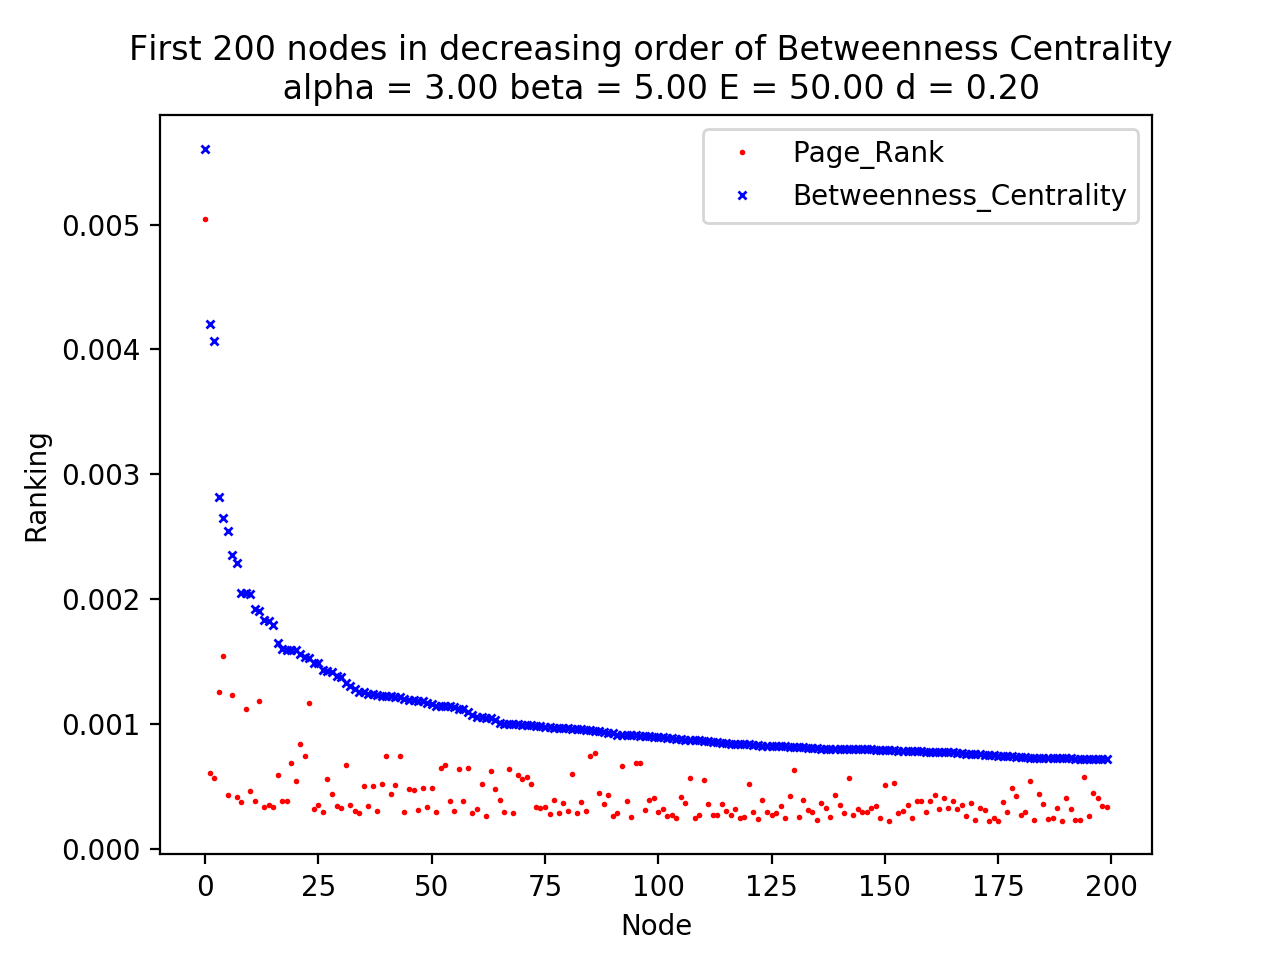
\includegraphics[width=8cm]{final_images/case2_m2_bcpr.png}}
\hfill
\subfigure[d=0.4]{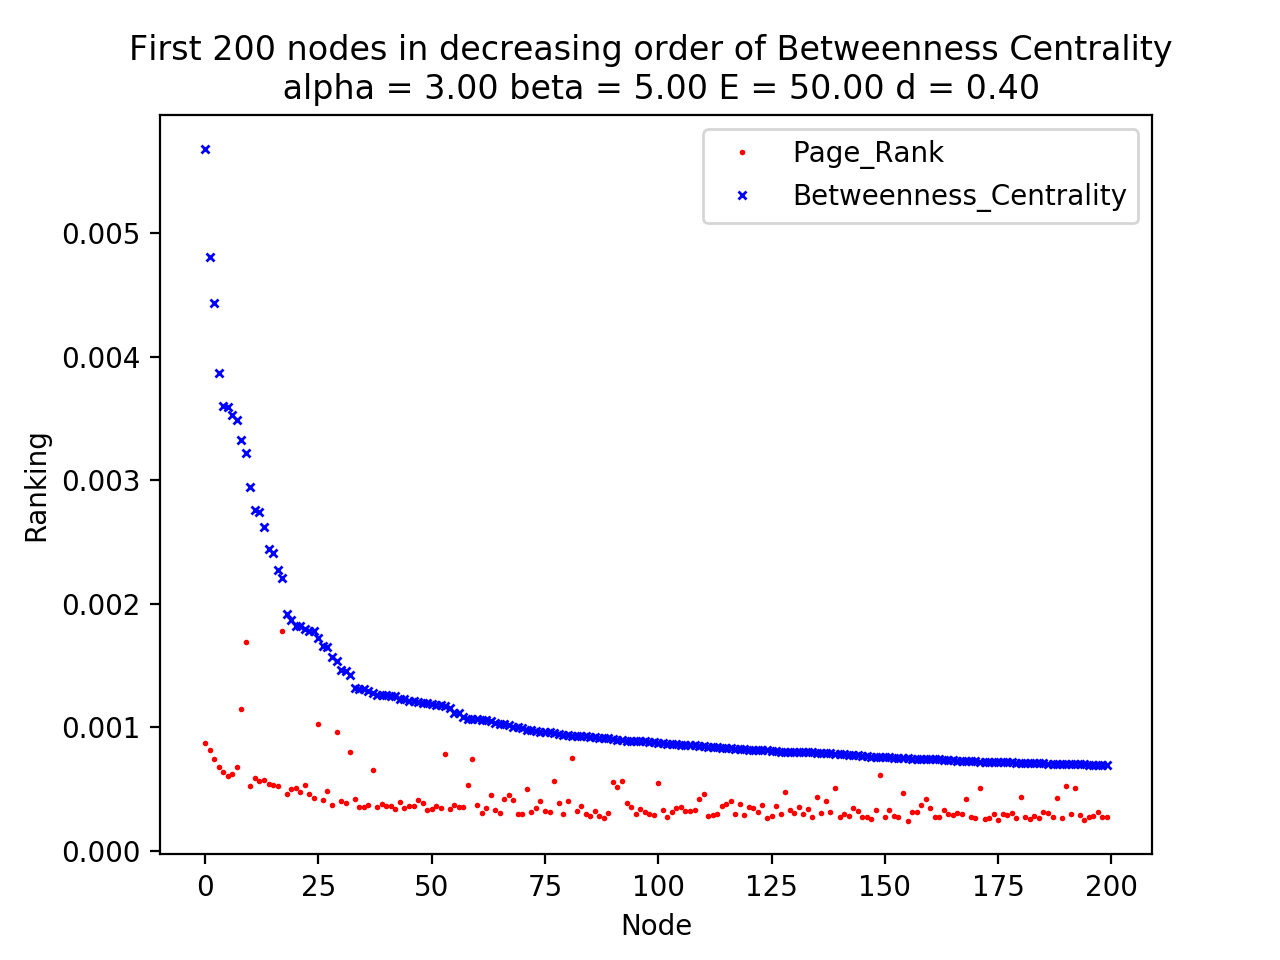
\includegraphics[width=8cm]{final_images/case2_m3_bcpr.png}}
\hfill
\subfigure[d=0.6]{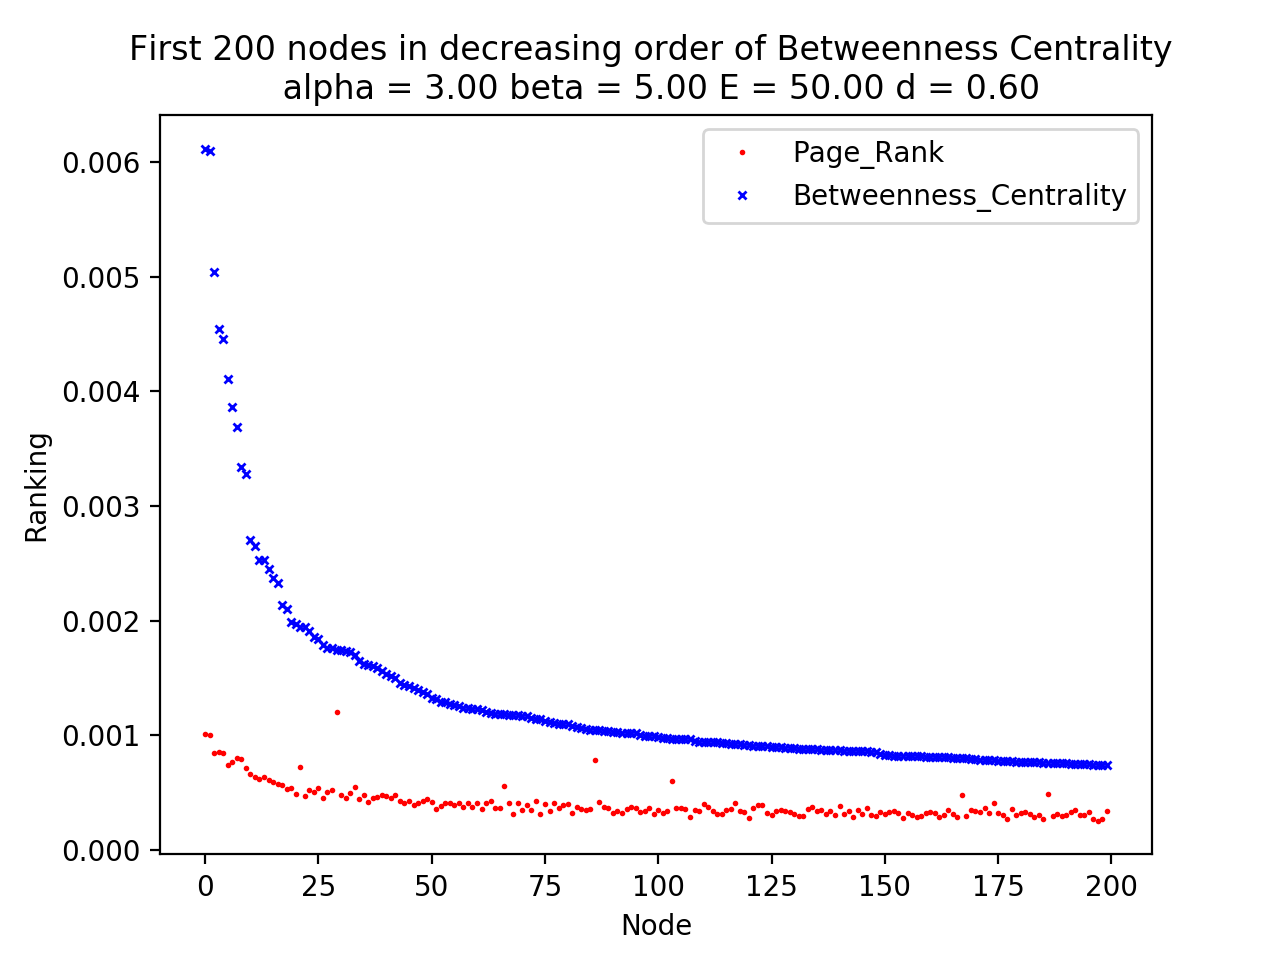
\includegraphics[width=8cm]{final_images/case2_m4_bcpr.png}}
\hfill
\subfigure[d=0.8]{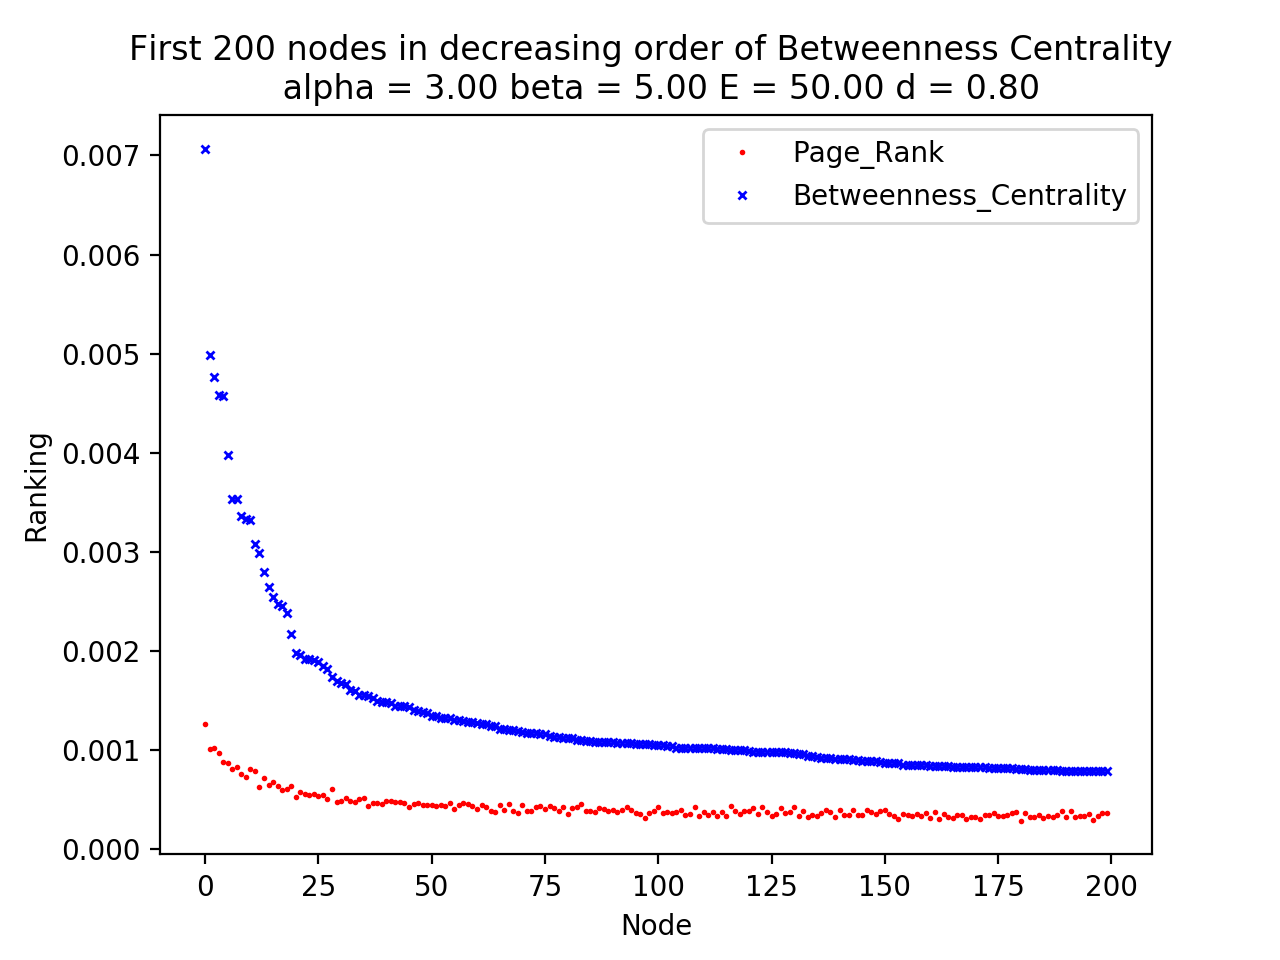
\includegraphics[width=8cm]{final_images/case2_m5_bcpr.png}}
\hfill
\subfigure[d=1.0]{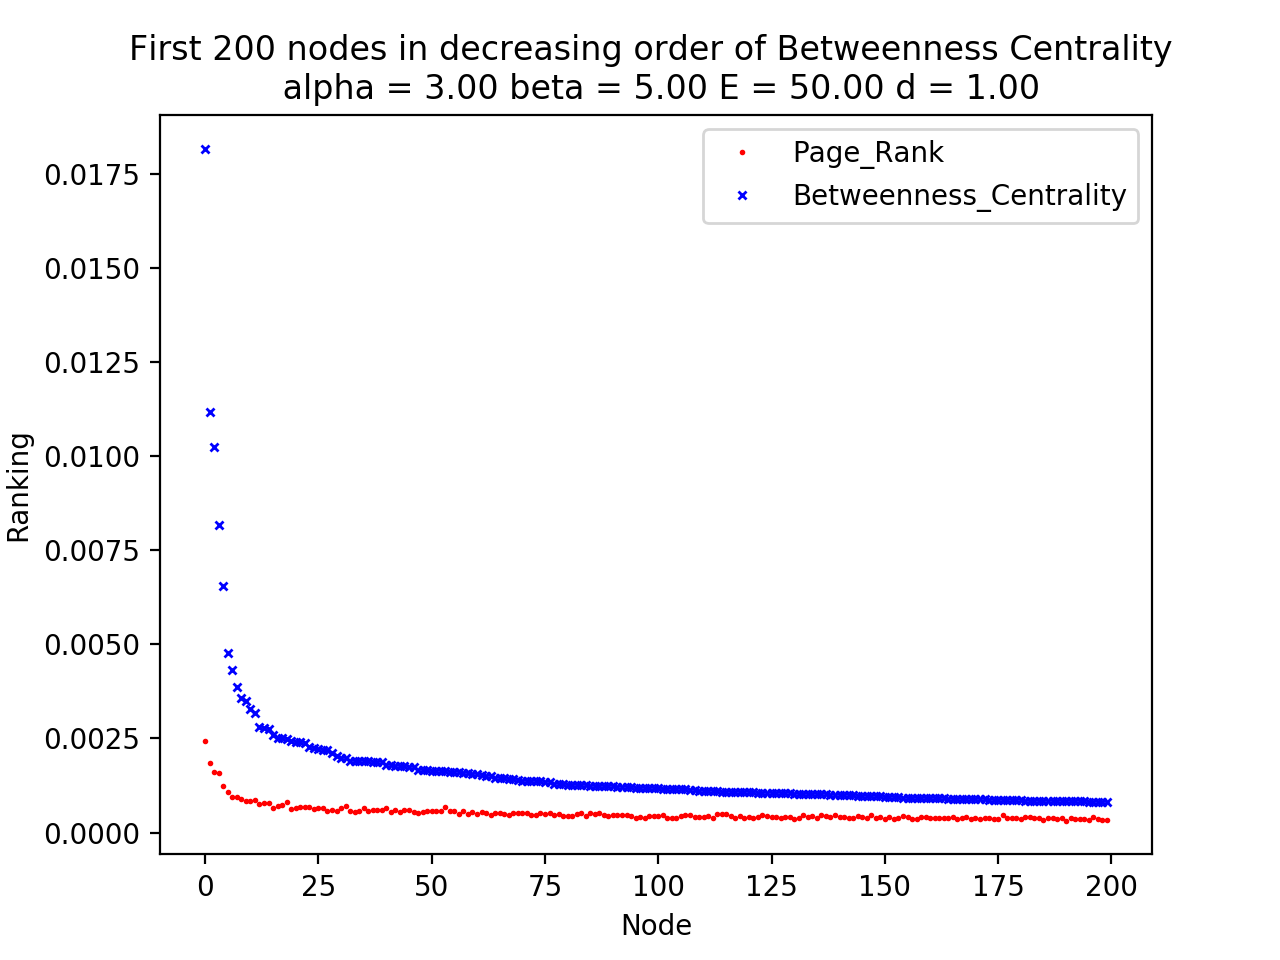
\includegraphics[width=8cm]{final_images/case2_m6_bcpr.png}}
\hfill
\caption{
\label{case2rankplotBC}%
Page Rank and Betweenness Centrality values of First 200 nodes in decreasing order of Betweenness Centrality}
\end{figure}

\par It is noteworthy that since the rank plot is plotted against a certain sample, it is a stochastic result. We plot 4 samples generated from one model to observe whether the trend in the plots vary much or not. \\
From Figure \ref{case2_4samples}, we could see that although the absolute rank( BC / PR) value of each node is different, but the behaviors of the scattered plot are similar.

\begin{figure}[!hbtp]
\hfill
\subfigure[Sample 1]{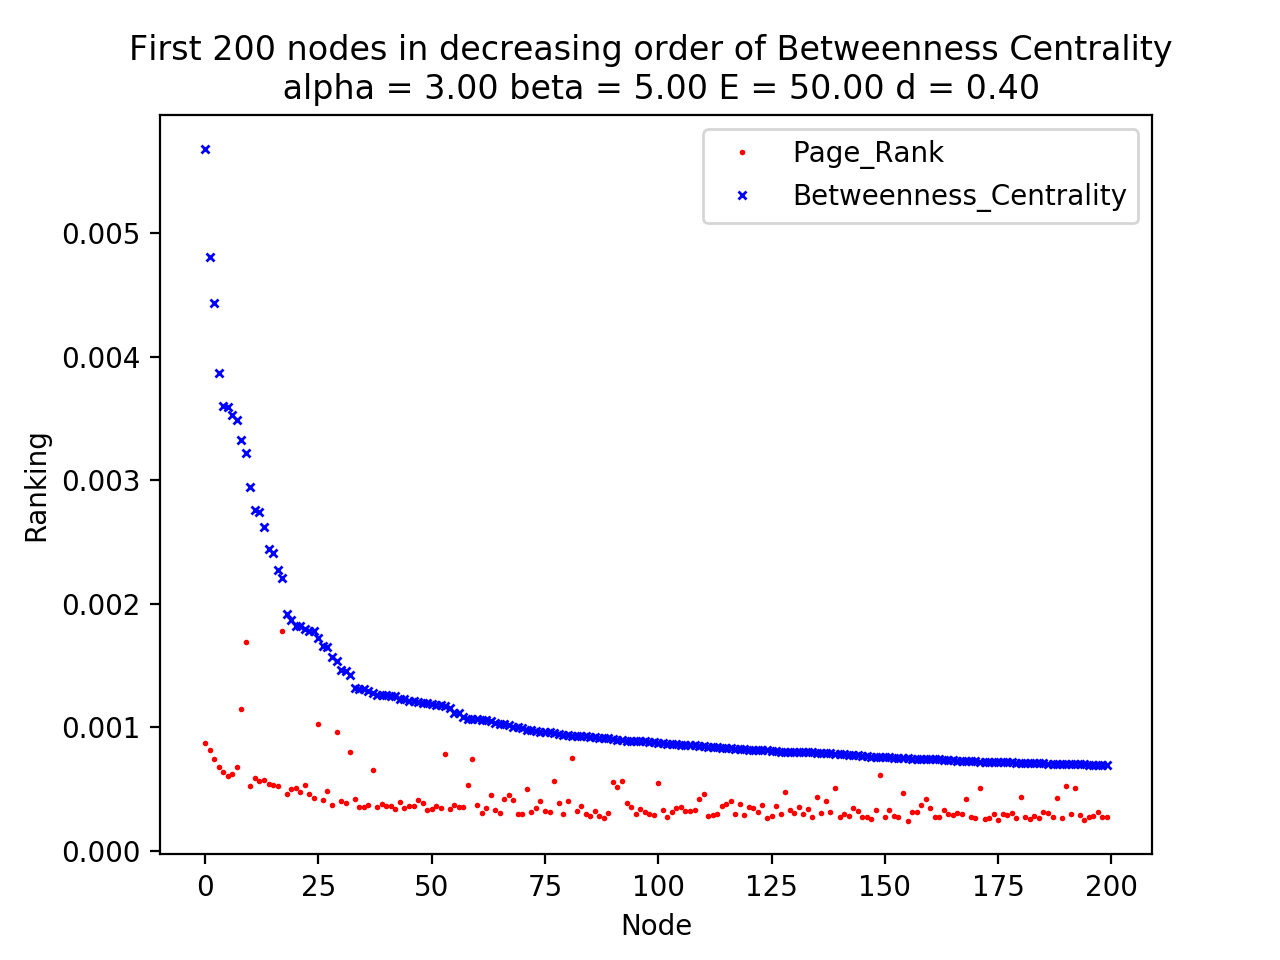
\includegraphics[width=8cm]{final_images/case2_m3_bcpr.png}}
\hfill
\subfigure[Sample 2]{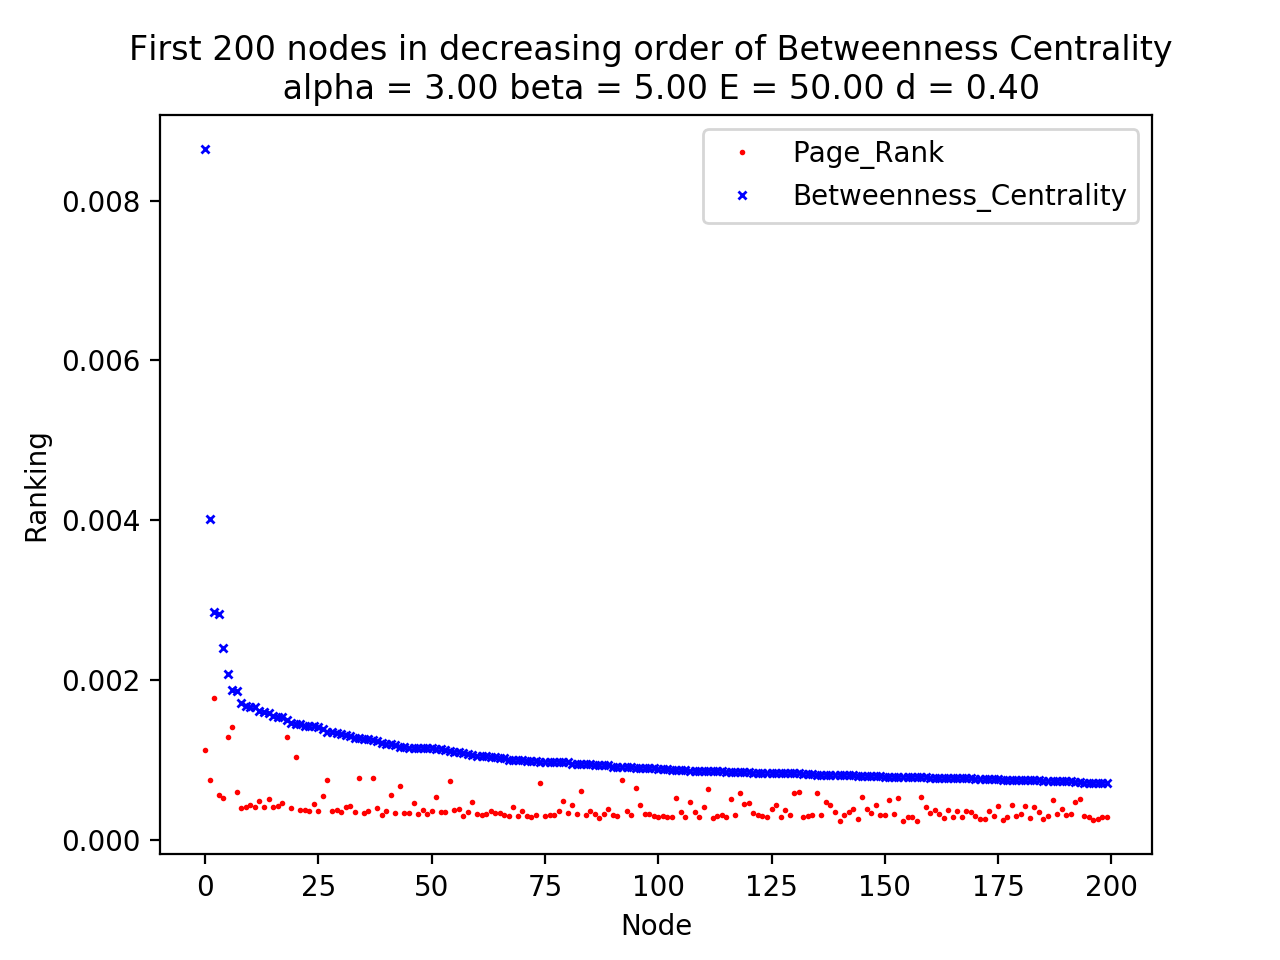
\includegraphics[width=8cm]{final_images/case2_m3_bcpr_alt1.png}}
\hfill
\subfigure[Sample 3]{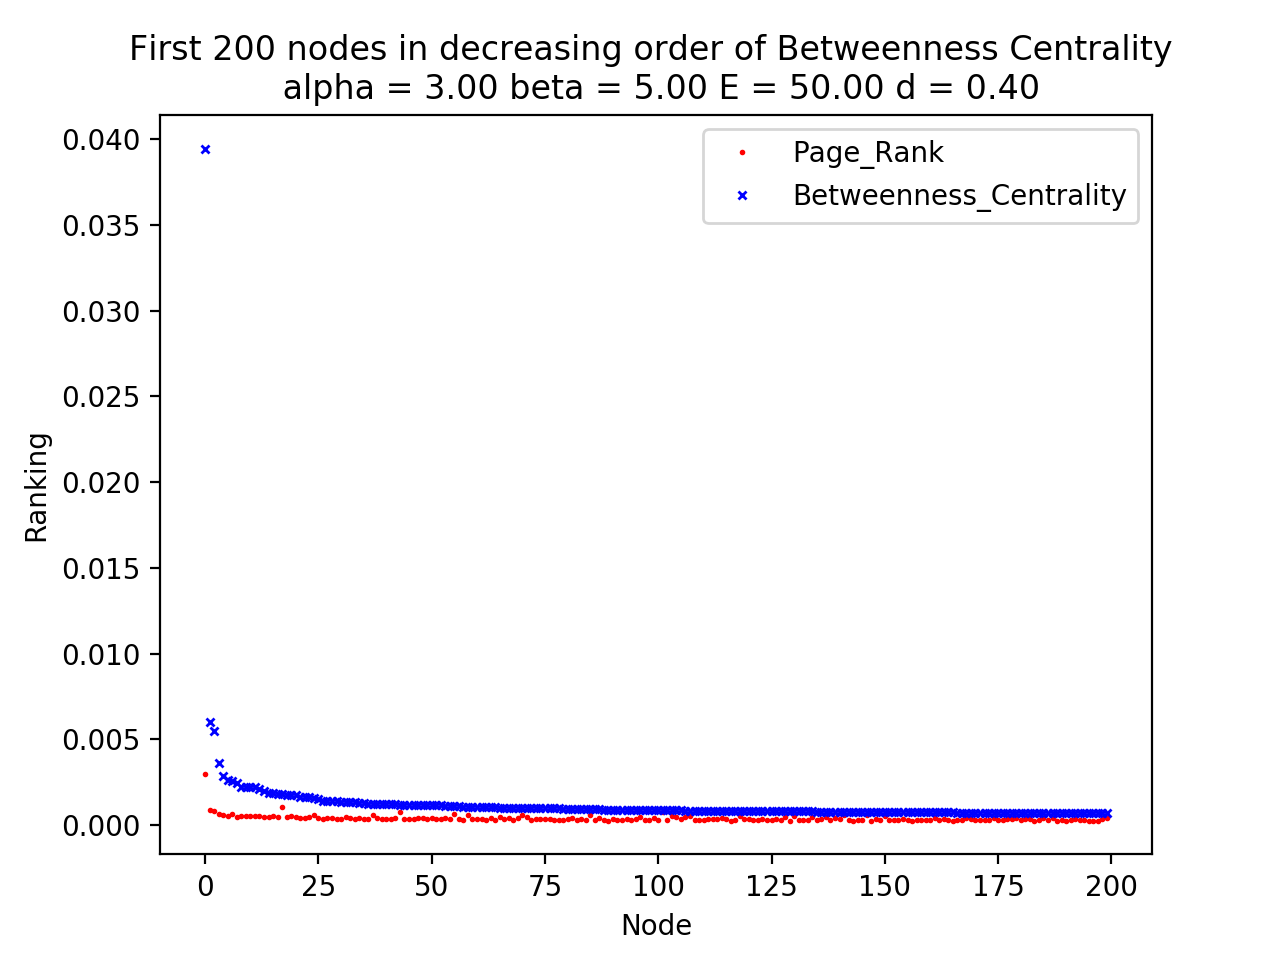
\includegraphics[width=8cm]{final_images/case2_m3_bcpr_alt2.png}}
\hfill
\subfigure[Sample 4]{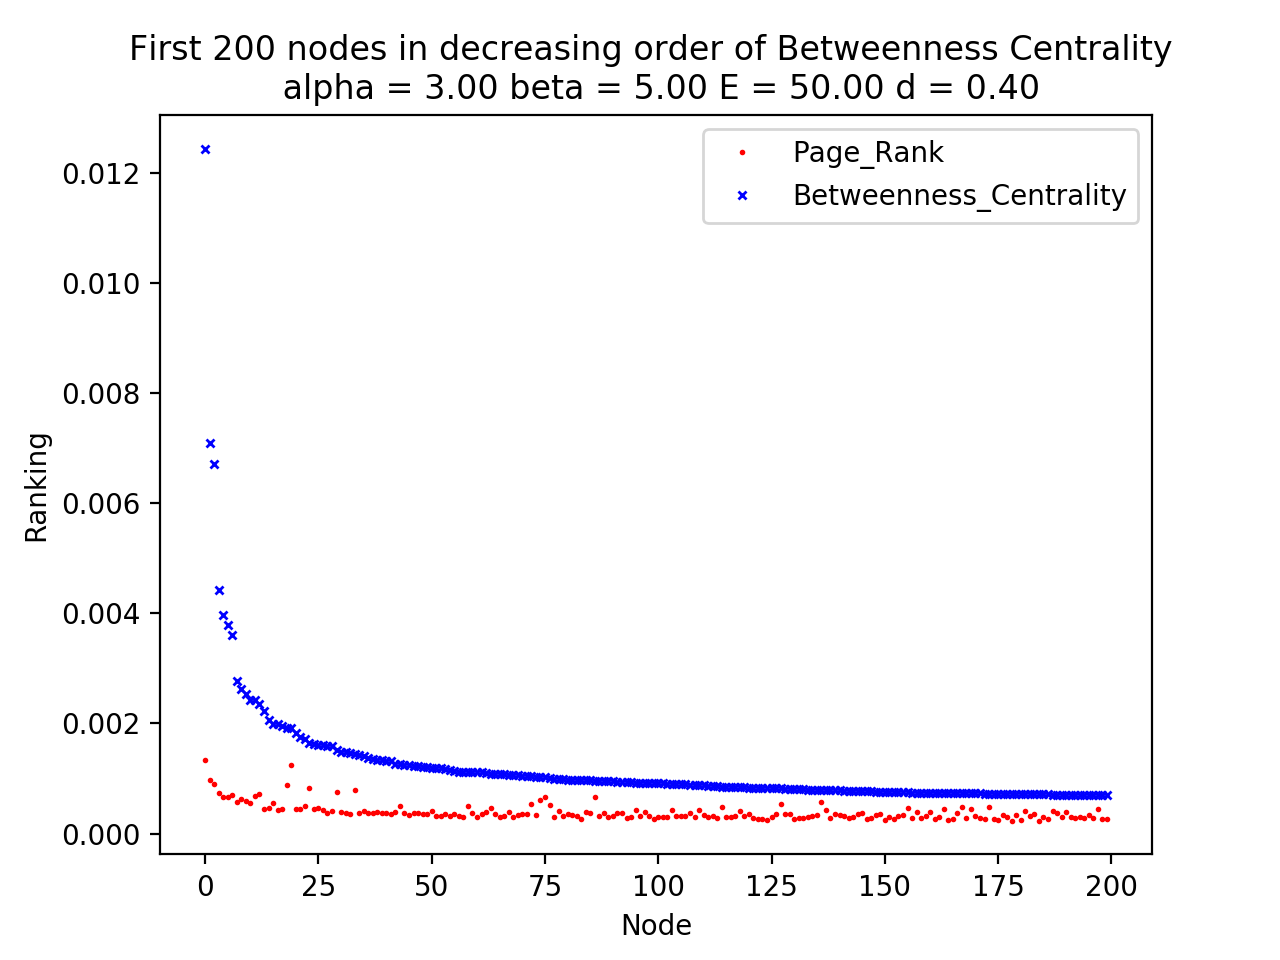
\includegraphics[width=8cm]{final_images/case2_m3_bcpr_alt3.png}}
\hfill
\caption{
\label{case2_4samples}%
4 samples from Model: $alpha=3, beta=5, E=50, d=0.40,  n=5000$}
\end{figure}



\item Rank Correlation
\begin{enumerate}

\item From Table \ref{table2}, we could see that the sample variance of rank correlation is close to 0, which suggests that the sample average of rank correlation is representative.
\item From Figure \ref{fig: corrs_2}, we could see as d increases,  degree correlation increases, and rank correlation increases.
\begin{table}[]
\centering
\caption{Case2 ($\alpha \neq \beta$): statistics of rank correlation over 20 samples}
\label{table2}
\begin{tabular}{|l|l|l|l|}
\hline
d   & computed degree correlation & average of rank correlation & variance of rank correlation \\
\hline
0   & 0                           & 0.770526926                            & 0.000107614 \\
\hline
0.2 & 0.195411751                & 0.820663736                            & 3.15524E-05 \\
\hline
0.4 &0.441451031                &0.856461981                            & 2.05965E-05
 \\
\hline
0.6 & 0.662176546                 & 0.880852803                         & 1.74735E-05
 \\
\hline
0.8 &0.781647004                & 0.899151153                           & 1.21308E-05
 \\
\hline
1.0 & 0.816363555                 & 0.915141277                             & 1.365E-05
\\
\hline
\end{tabular}
\end{table}


\begin{figure}
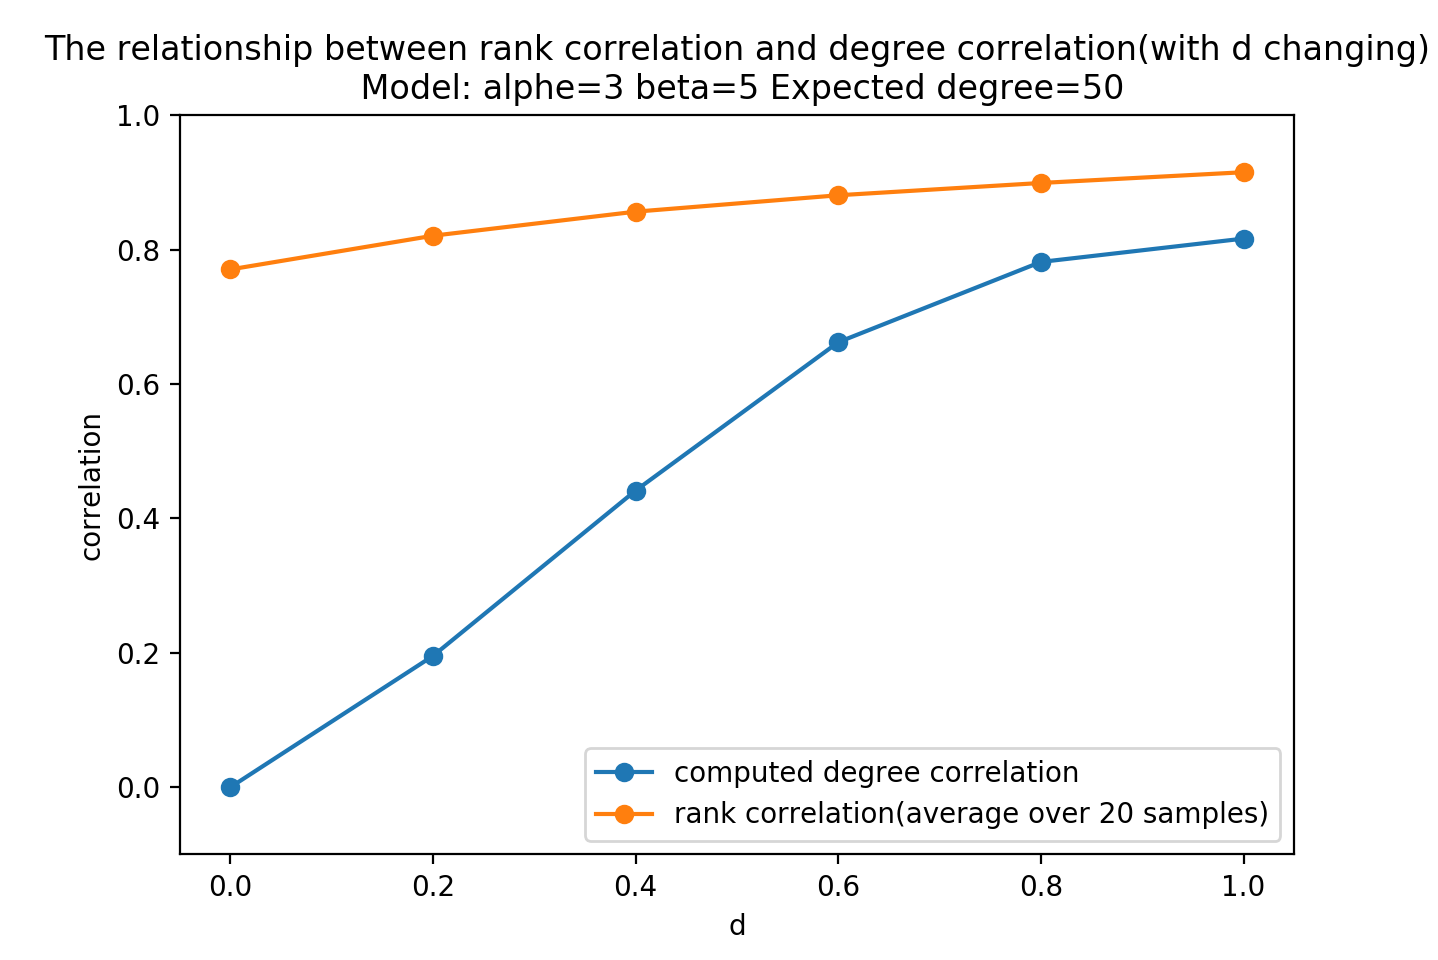
\includegraphics[scale=1]{final_images/case2_corrs_relation.png}
\caption{Case2($\alpha \neq \beta$): relationship between rank correlation and degree correlation}
\label{fig: corrs_2}
\end{figure}

\end{enumerate}

\end{enumerate}

\subsection{Conclusions}
\begin{enumerate}
\item Rank correlation over a certain amout of samples, and rank plot of a sample, is representative. Especially for the former, the variance over 20 samples is very close to 0, whis means the sample rank correlation is very stablized and close to expected value.
\item As the degree correlation increases (by adjusting the value of $d$), the correlation between Page Rank and Betweenness Centrality increases.
\end{enumerate}

\section{Part 2:  Comparison among the effect of Measures on Average Shortest Path Length}
\par In this section,  we want to compare among different ranking algorithms / measures of importance (PR, BC, total degree, in-degree, out-degree) with respect to graph connectivity efficiency. For a graph G, we choose the Average Shortest Path Length (ASPL) as the indicator of its connectivity efficiency. 

\subsection{Method Description}
\par In procedure, we consecutively eliminate the individual node based on different m\par easures and compute the corresponding ASPL, thus deriving the effect from higher ranking nodes. Note that each time we eliminate a node, we use the remnant graph's strongly connected component(SCC) to calculate the new ASPL, since the compuation of ASPL requires the graph to be connected. After consecutively eliminating $m$ nodes, we could obtain a numeric array of ASPL of length $m$ with respect to one specific ranking algorithm's measure. Independently conducting the procedure w.r.t. each ranking measure,  we can make the plot as in Figure \ref{repetitions}: the ranking of the lines from top to down suggest the ranking of the effect on ASPL. 
\par Due to the randomness of the graph, there is noise in the simulated graph's ASPL. Therefore, we repeatedly conduct the model simulation and take the average of each simulation's shortest to smooth out the noise.

\subsection{Experiment and Analysis}

\subsubsection{Theoretical Models}

\par As we do in Part 1 to vary the degree correlation, we let $d$ range from 0 to 1 with step size 0.25. And the other parameters to fix the model are: $\alpha$ = 2.1, $\beta$ = 3, the expected degree E = 3, the node size of graph n = 5000. We consecutively eliminate 100 nodes and independently repeat the prcedure for 5 times and then compute the average.

\begin{enumerate}
\item Noises in ASPL\\

\par The noise can be clearly observed in the first 5 plots ((a) to (e)) in Figure \ref{repetitions}. The n-th Pagerank and out-degree ranking even switch the ordering in different realization, which suggests the vacillation.  Plot (f) in Figure  \ref{repetitions} is the average effect of the foregoing five independent repetitions, which smoothes out the noise. Moreover, it denotes that ASPL is most sensitive to BC, which makes sense since BC is a measure of centrality. However, it seems that PageRank fails to capture the ASPL characteristics. \\

\begin{figure}[!hbtp]
\hfill
\subfigure[Repetition(1)]{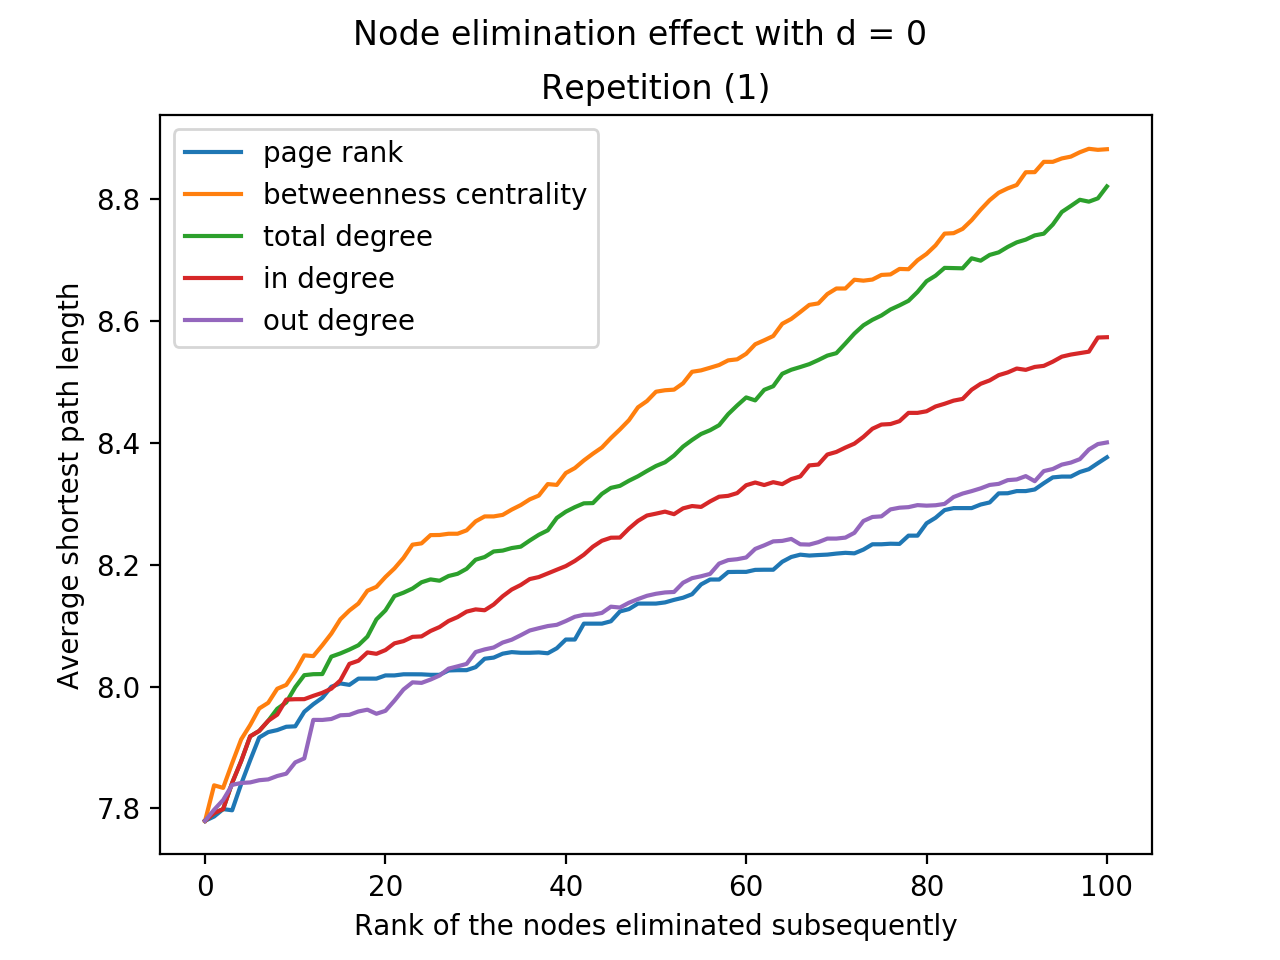
\includegraphics[width=8cm]{final_images/0d1.png}}
\hfill
\subfigure[Repetition(2)]{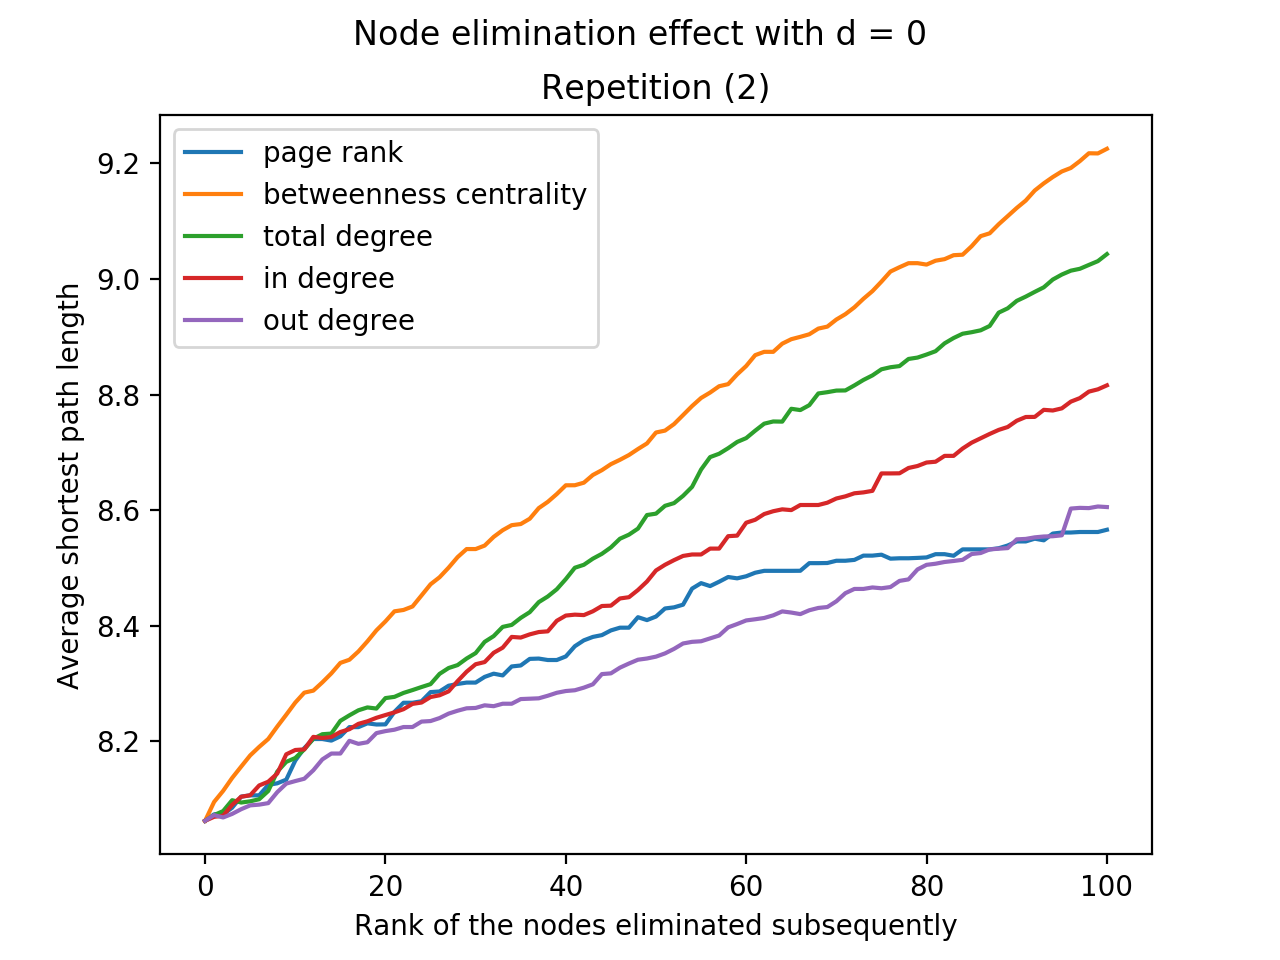
\includegraphics[width=8cm]{final_images/0d2.png}}
\hfill
\subfigure[Repetition(3)]{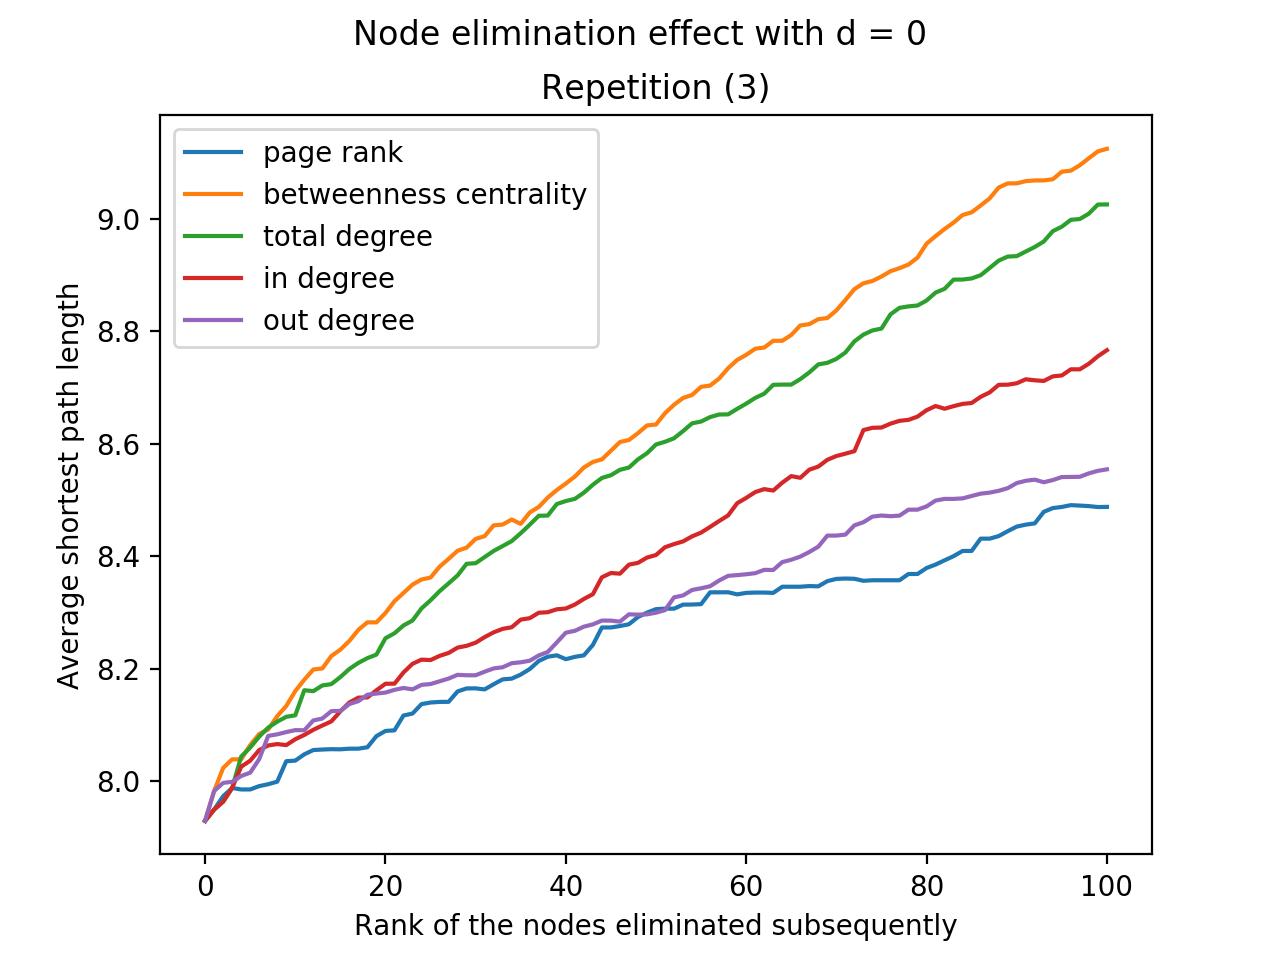
\includegraphics[width=8cm]{final_images/0d3.png}}
\hfill
\subfigure[Repetition(4)]{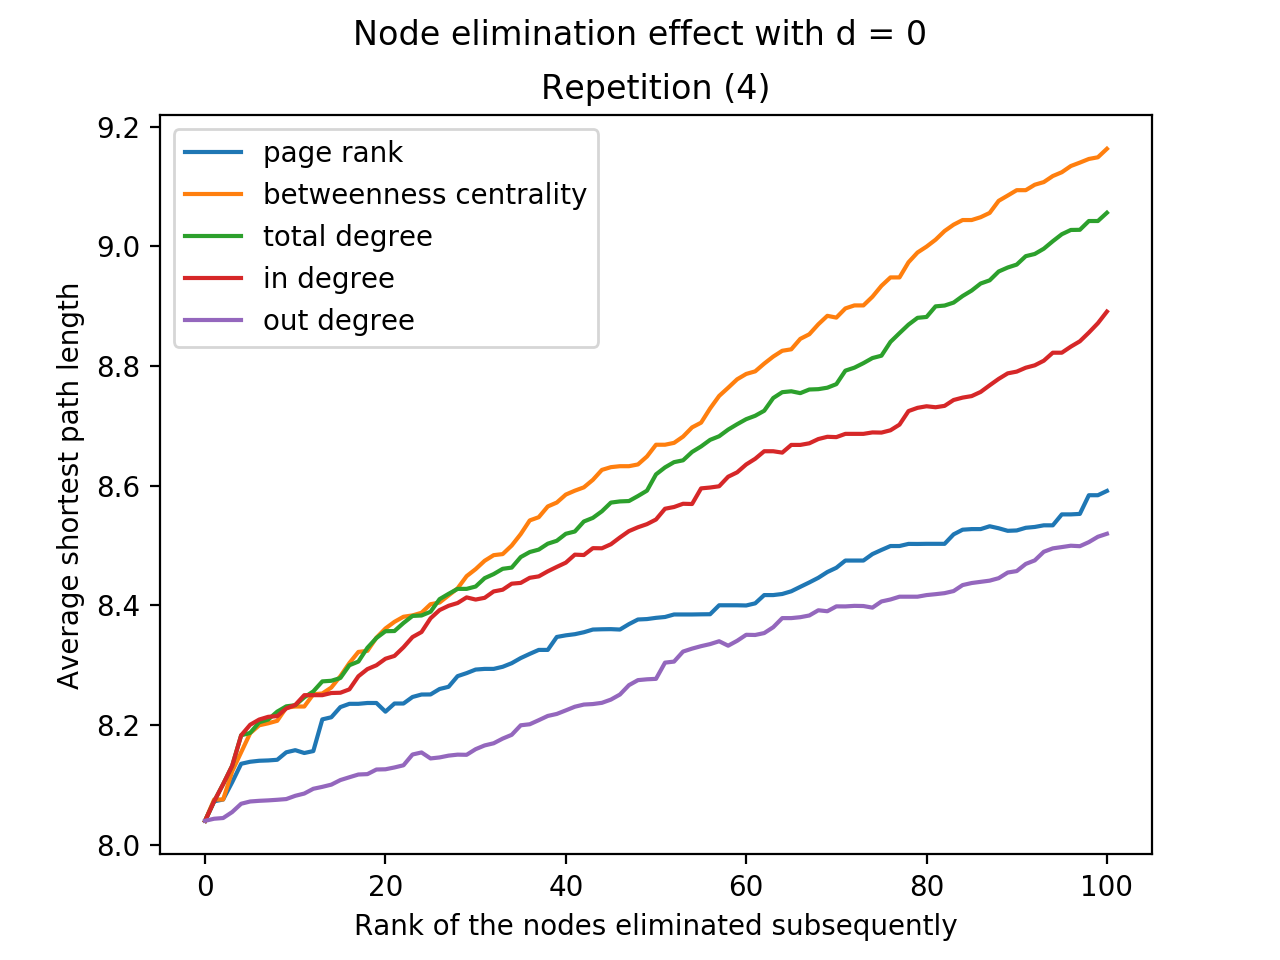
\includegraphics[width=8cm]{final_images/0d4.png}}
\hfill
\subfigure[Repetition(5)]{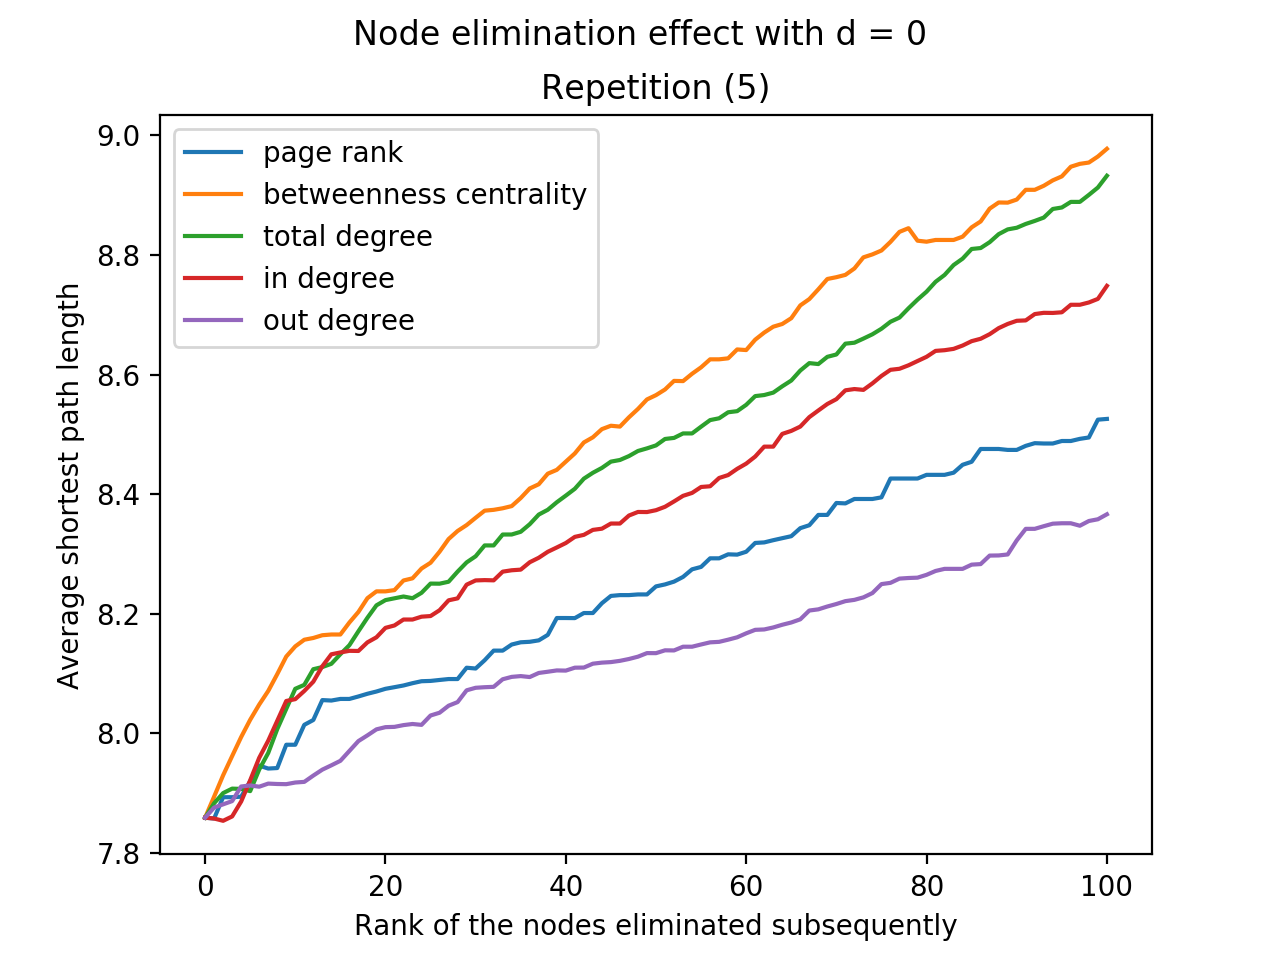
\includegraphics[width=8cm]{final_images/0d5.png}}
\hfill
\subfigure[Average over 5 repetitions)]{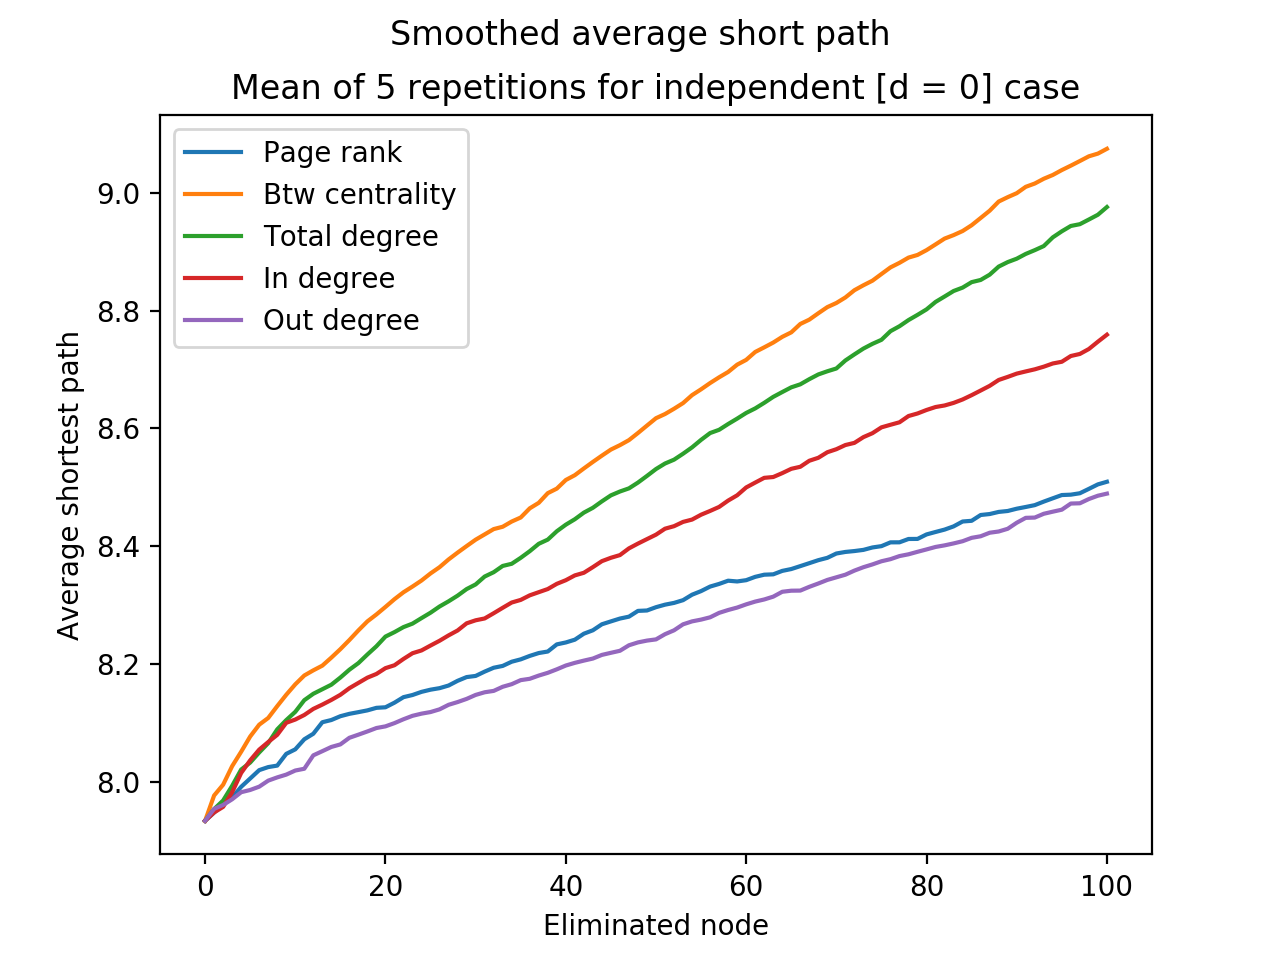
\includegraphics[width=8cm]{final_images/avgd0.png}}
\hfill
\caption{
\label{repetitions}%
 Repetitive Model Simulation and the Average Effect ( d = 0)}
\end{figure}

\item Effect of Measures on ASPL in Different dependence levels\\

\par In order to check the ASPL change in different dependence (degree correlation) level, we assign d with value from five levels: 0, 0.25, 0.5, 0.75 and 1. And to smooth out the noise, in each dependence level case we simulate models by five replications and then plot the average. Since when $d = 1$ we fail to get a correlation eauals to 1, we add the case that in-degree sequence is identical to out-degree sequence so that degree correlaiton equals to 1. The code in this case is:

\begin{lstlisting}
w_plus = generate_w(self.c, self.alpha)
d_plus= int(poisson(mu=w_plus).rvs())
d_minus = d_plus
\end{lstlisting}
so that both in and out degree sequence have power law distribution with index $alpha$.

\begin{figure}[!hbtp]
\hfill
\subfigure[d = 0.00 corr = 0]{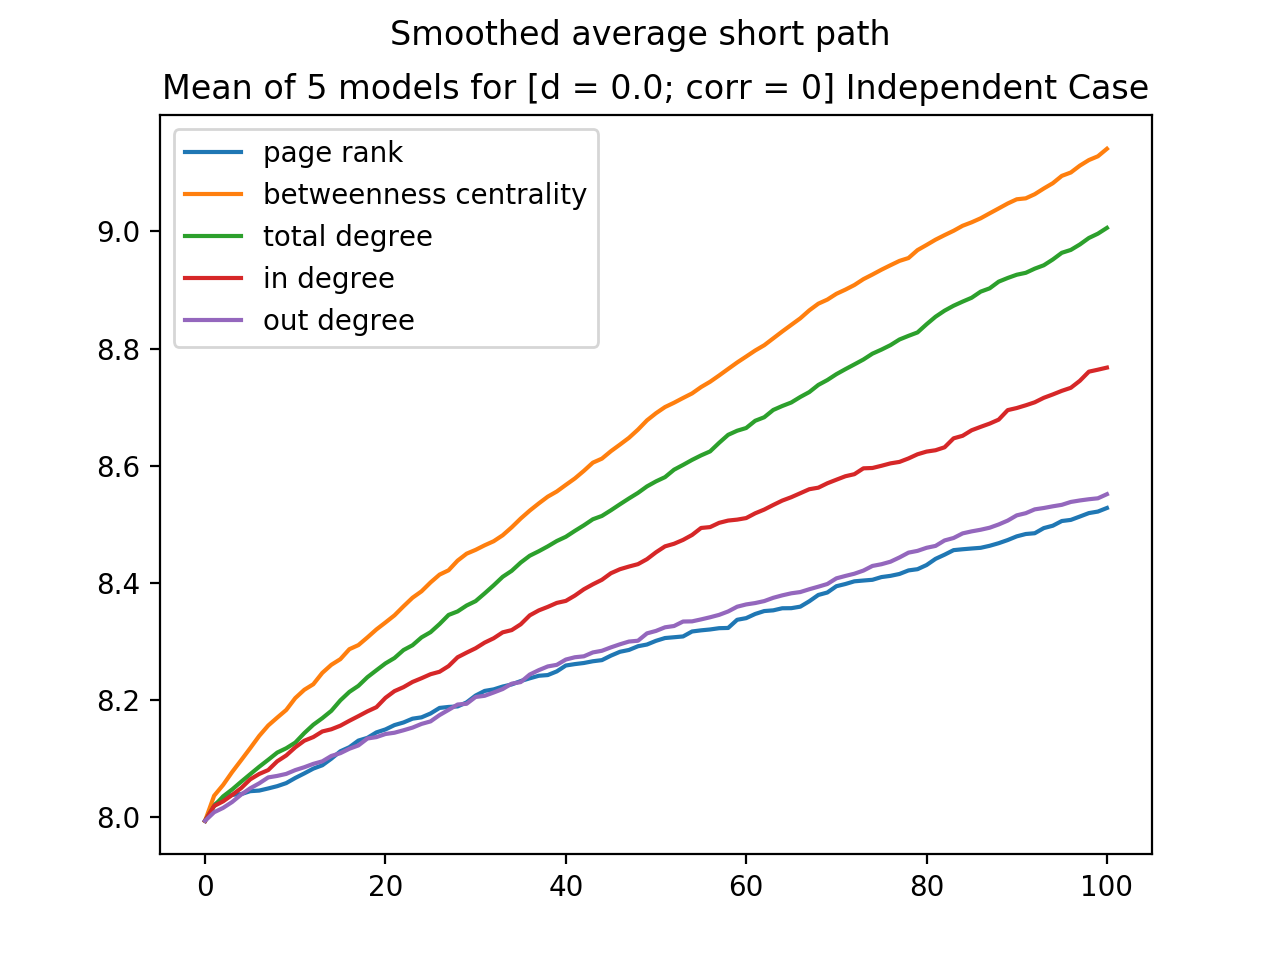
\includegraphics[width=8cm]{final_images/d00.png}}
\hfill
\subfigure[d = 0.25 corr = 0.140]{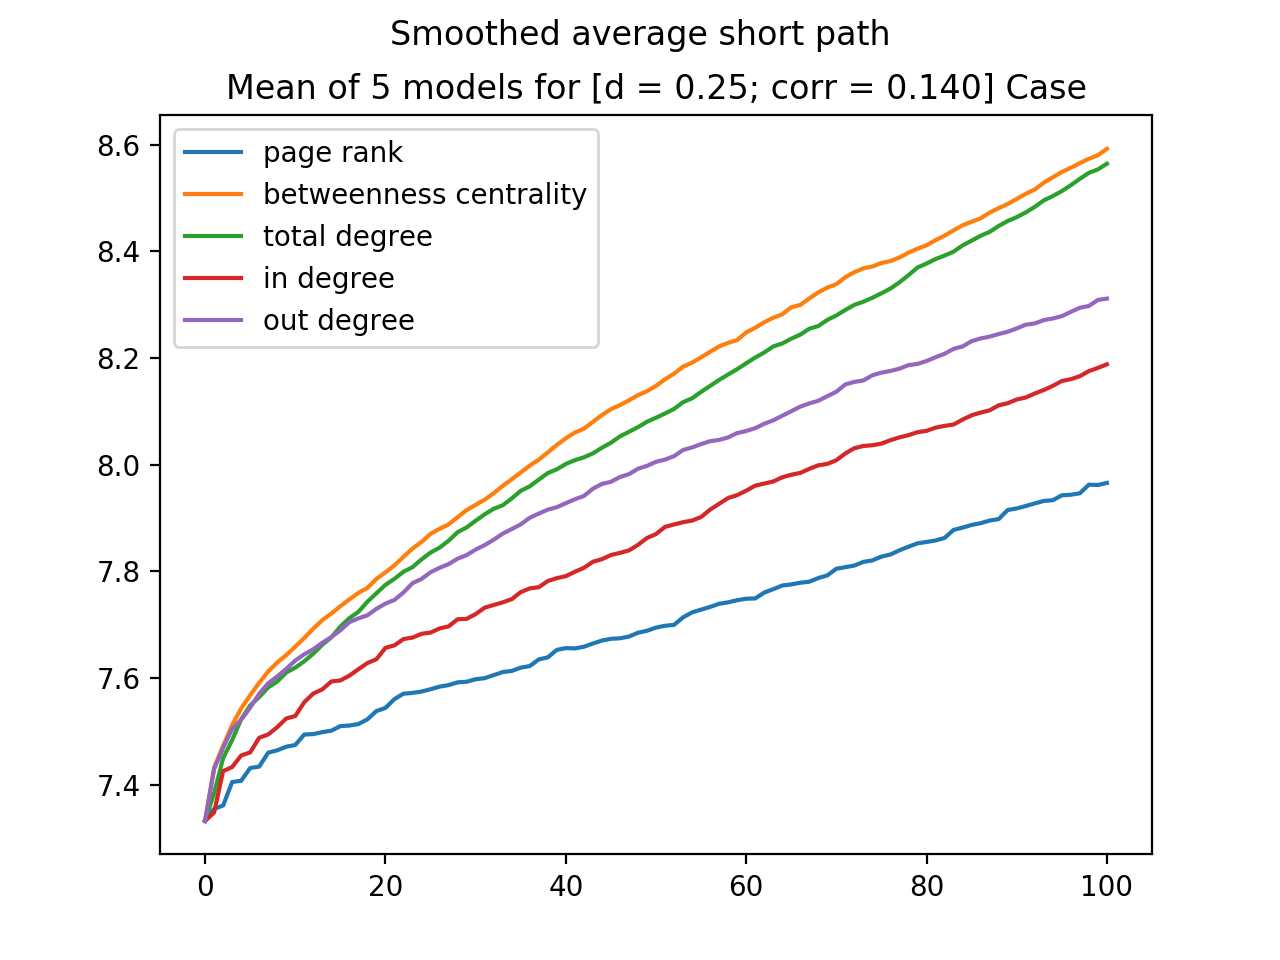
\includegraphics[width=8cm]{final_images/d25.png}}
\hfill
\subfigure[d = 0.50 corr = 0.310]{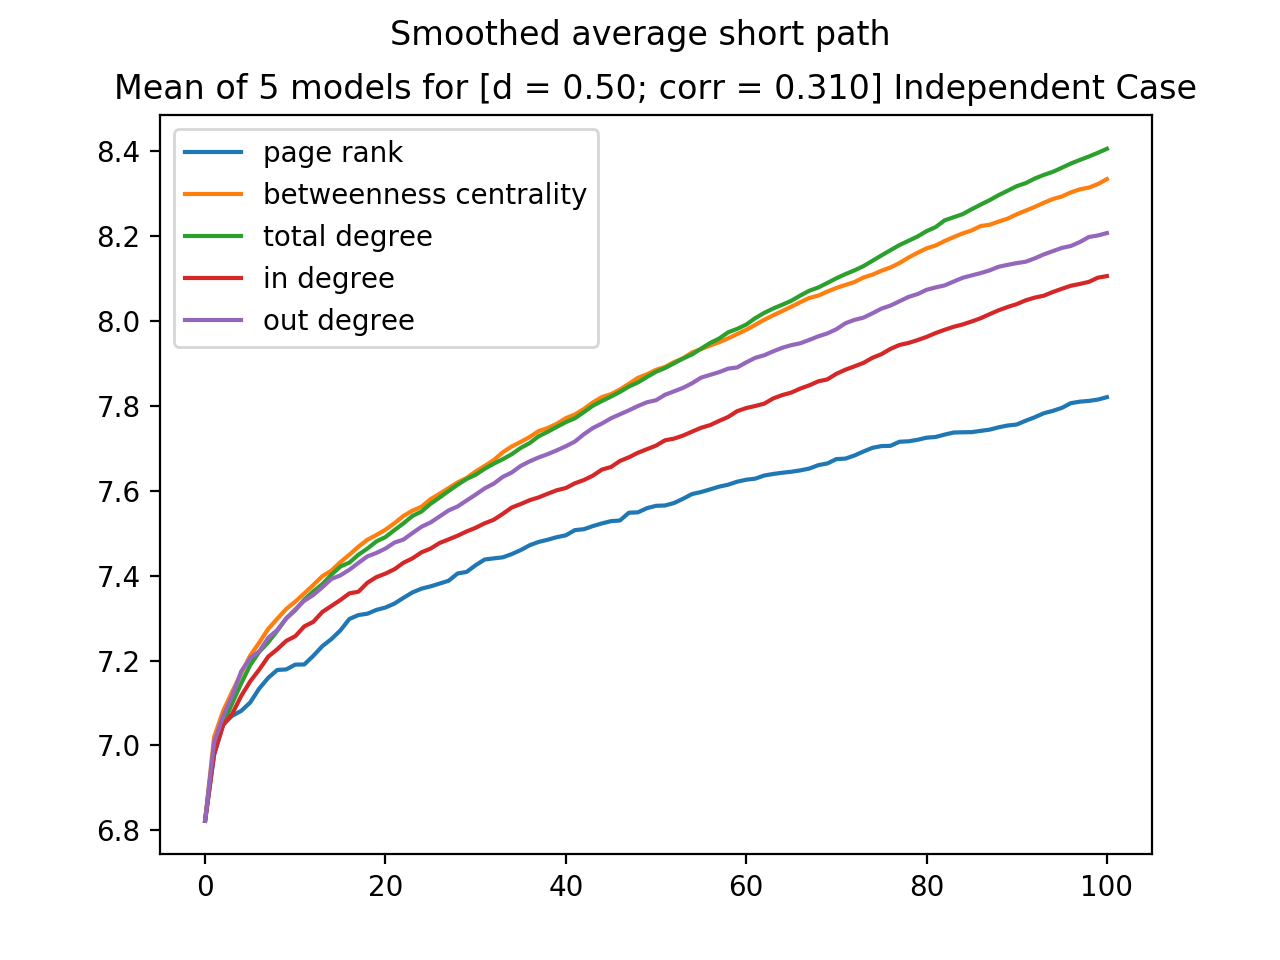
\includegraphics[width=8cm]{final_images/d50.png}}
\hfill
\subfigure[d = 0.75 corr = 0.421]{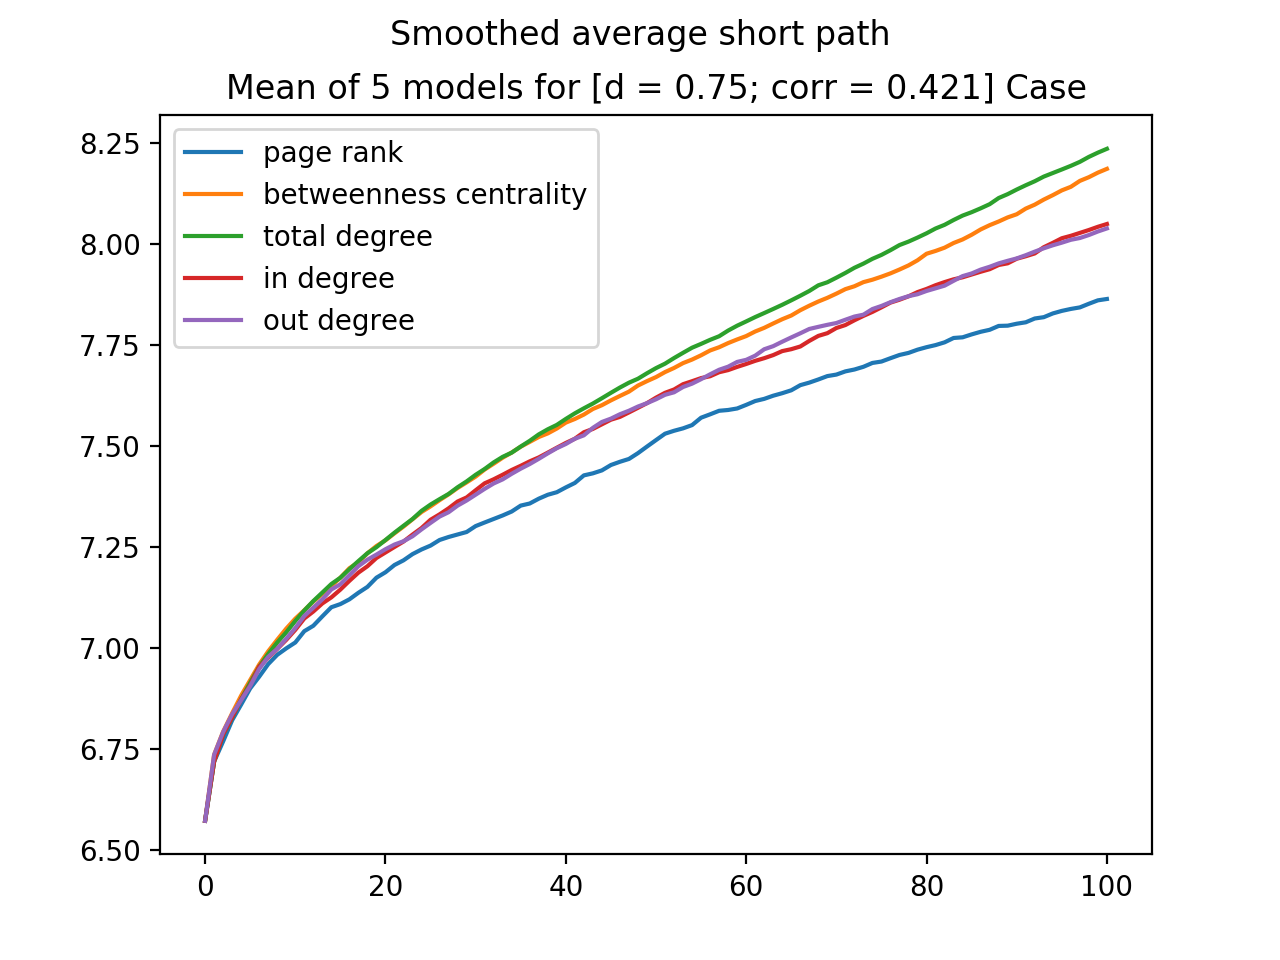
\includegraphics[width=8cm]{final_images/d75.png}}
\hfill
\subfigure[d = 1.00 corr = 0.452]{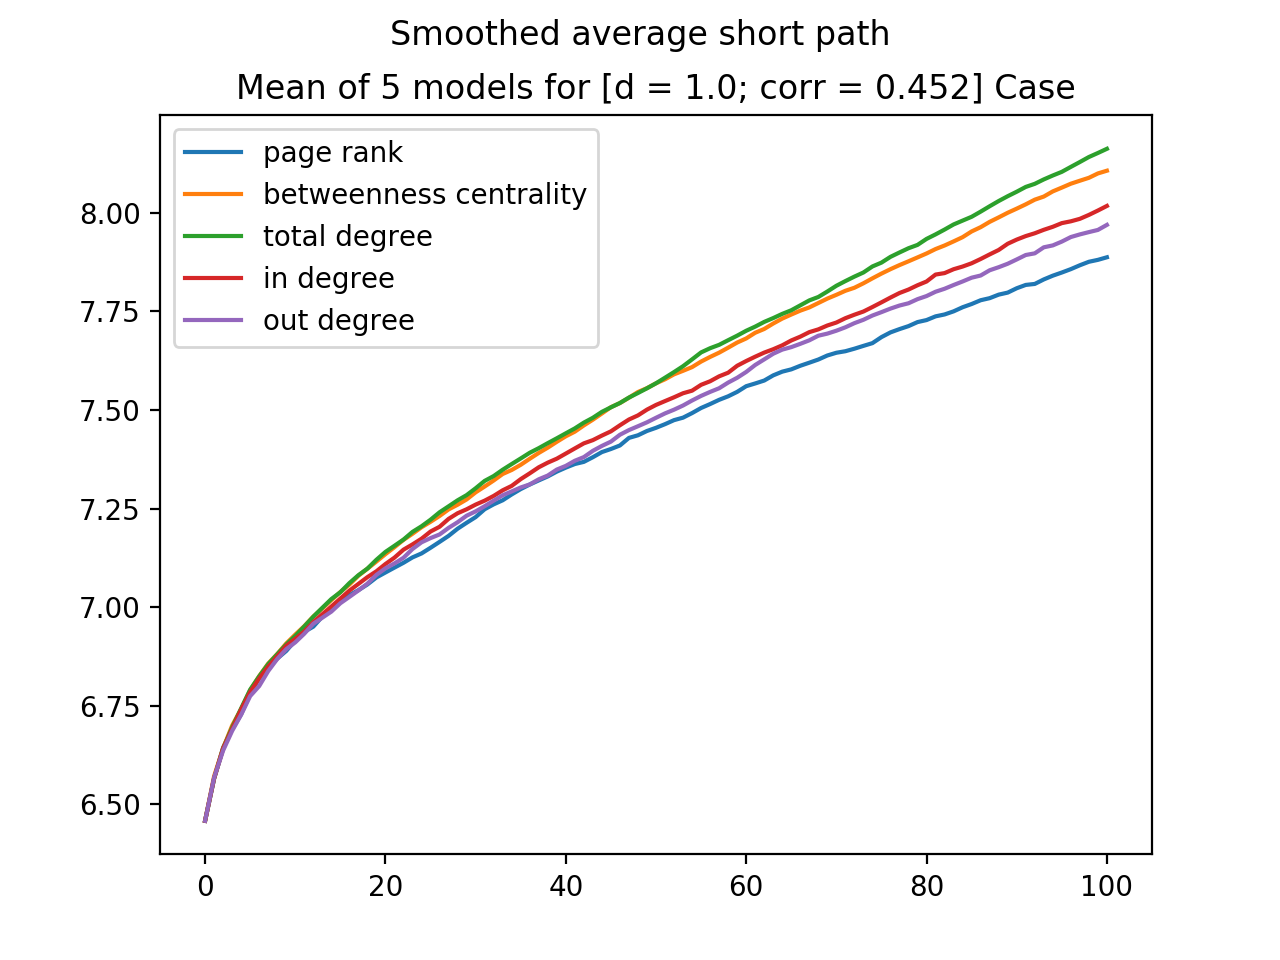
\includegraphics[width=8cm]{final_images/d100.png}}
\hfill
\subfigure[perfectedly correlated  corr = 1(in degree sequence = out degree sequence)]{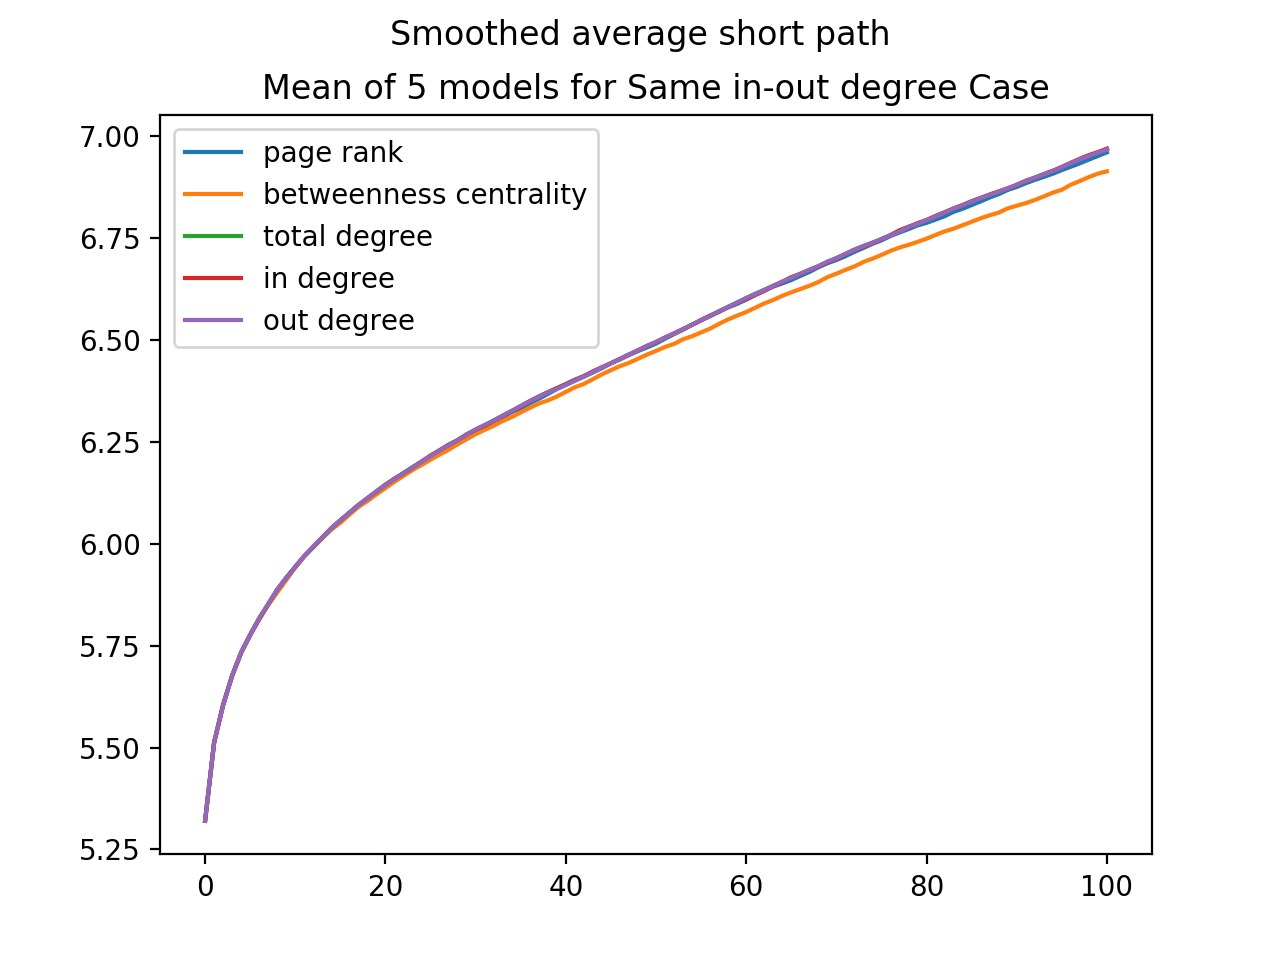
\includegraphics[width=8cm]{final_images/avgsam.png}}
\hfill
\caption{
\label{comps}%
Comparison of Effect on ASPL in Different Degree Correlation Levels}
\end{figure}

From Figure \ref{comps}, we have following observations:
\begin{enumerate}
\item As degree correlation increases, the five lines are getting closer, which suggests the effect of each measures is more similar.
\item From (a) to (e), the ranking of effect ( judged by the line from top to bottom) is: BC/total degree -- in-degree/out-degree -- Pararank.
\item In (f), that is the perfectly-correlated case, all measures except BC has similar, top effect.
\end{enumerate}

\end{enumerate}

\subsubsection{Real World Graph: Wikipedia Vote Network}
\par To testify the numerical study, we apply the experiment to real world data. 

\begin{enumerate}
\item Introduction of Wiki-Vote Network\\

\par In consideration of the directed configuration graph model feature, we select the \hyperlink{wikivote_intro}{Wikipedia vote network} from \href{https://snap.stanford.edu/data/}{Stanford Large Network Dataset Collection}, which is a directed graph. 
\par The statistics of the graph data is shown in Table \ref{wikivote_stats}.
\quad\\
\begin{table}[!hbp]
\centering
\caption{Wikipedia vote network statistics}\label{wikivote_stats}
\begin{tabular}{cc}

\toprule
Feature name & Value\\
\midrule
Nodes size & 7115\\
Edges & 103689\\
Expected degree & 14.57\\
In-out degree correlation & 0.317\\
Average clustering coefficient & 0.1409\\
Number of triangles & 608389\\
Diameter(longest shortest path) & 7\\

\bottomrule

\cline{1-2}
\hline
\end{tabular}
\end{table}
\\
\quad\\

\item Fitting Wiki-Vote Network into Theoretical Model\\

\par To determine whether Wiki-vote network has scale-free property (power law degree distribution), and what are the indices if it has, we make the log-log plot of the tail-distribution of in-degree and out-degree sequence, and Lease-Square-Estimate to fit the tail. \hypertarget{powerlaw_fit}{The fitting result} is shown in Figure  :$alpha =
3.5, \beta = 2.5$,  since we have $E$ = 14.57, in-out degree correlation = 0.317, we can substitue the values into the degree correlation formula to get $d$ = 0.339. 


\begin{figure}[!htbp]
\label{wikivote_fit}
\centering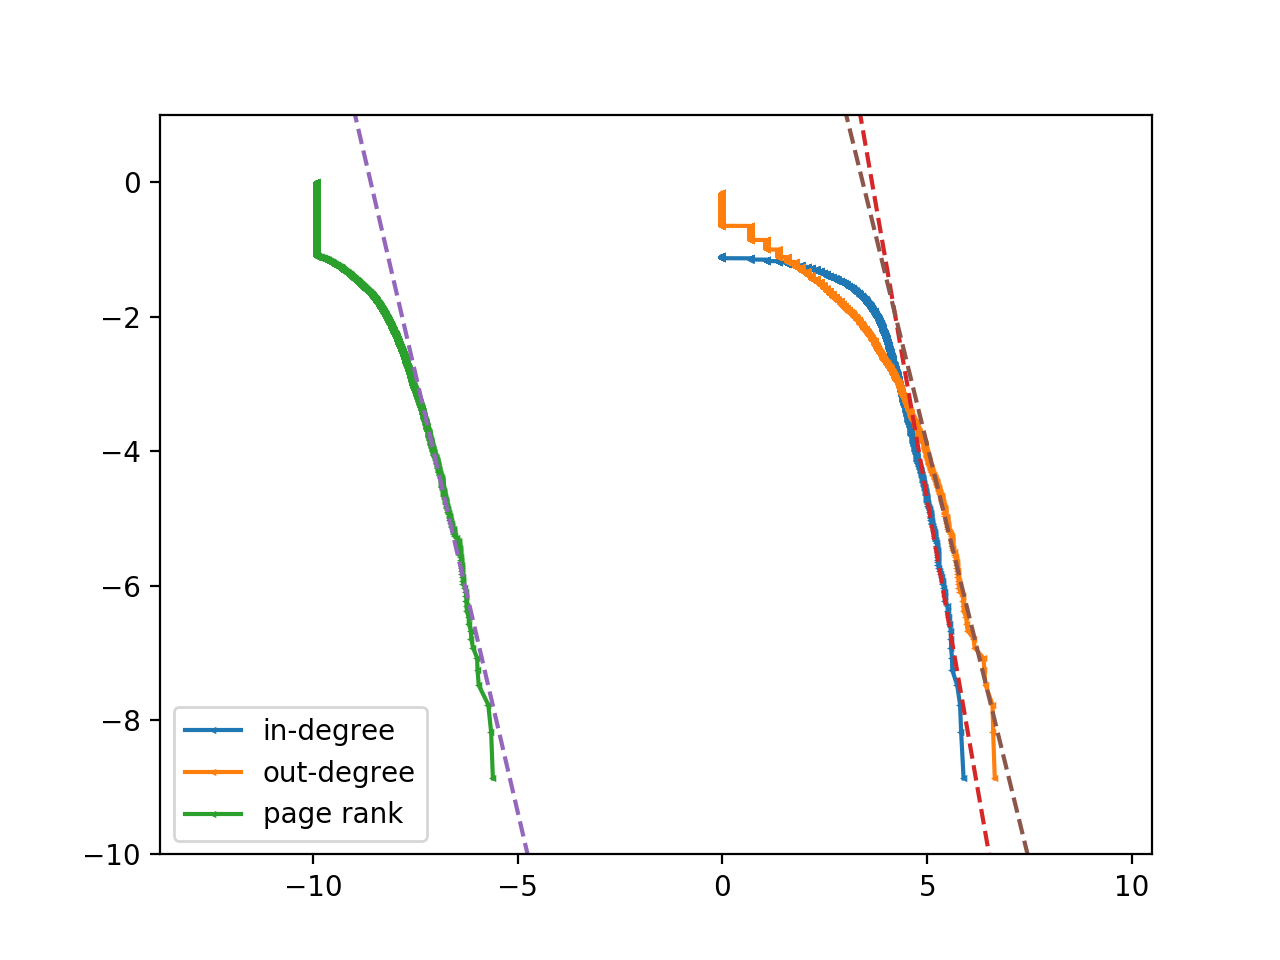
\includegraphics[width=10cm, height=8cm]{final_images/wiki_vote_fit1.png}
\caption{log-log plot of tail distribution of Wiki-vote network}
\end{figure}

\item Node Elimination effect on Wiki-Vote network\\

\par The node elimination effect on real graph's average shortest path length is shown in Figure \ref{wikivote_elim}.

\begin{figure}[!htbp]
\centering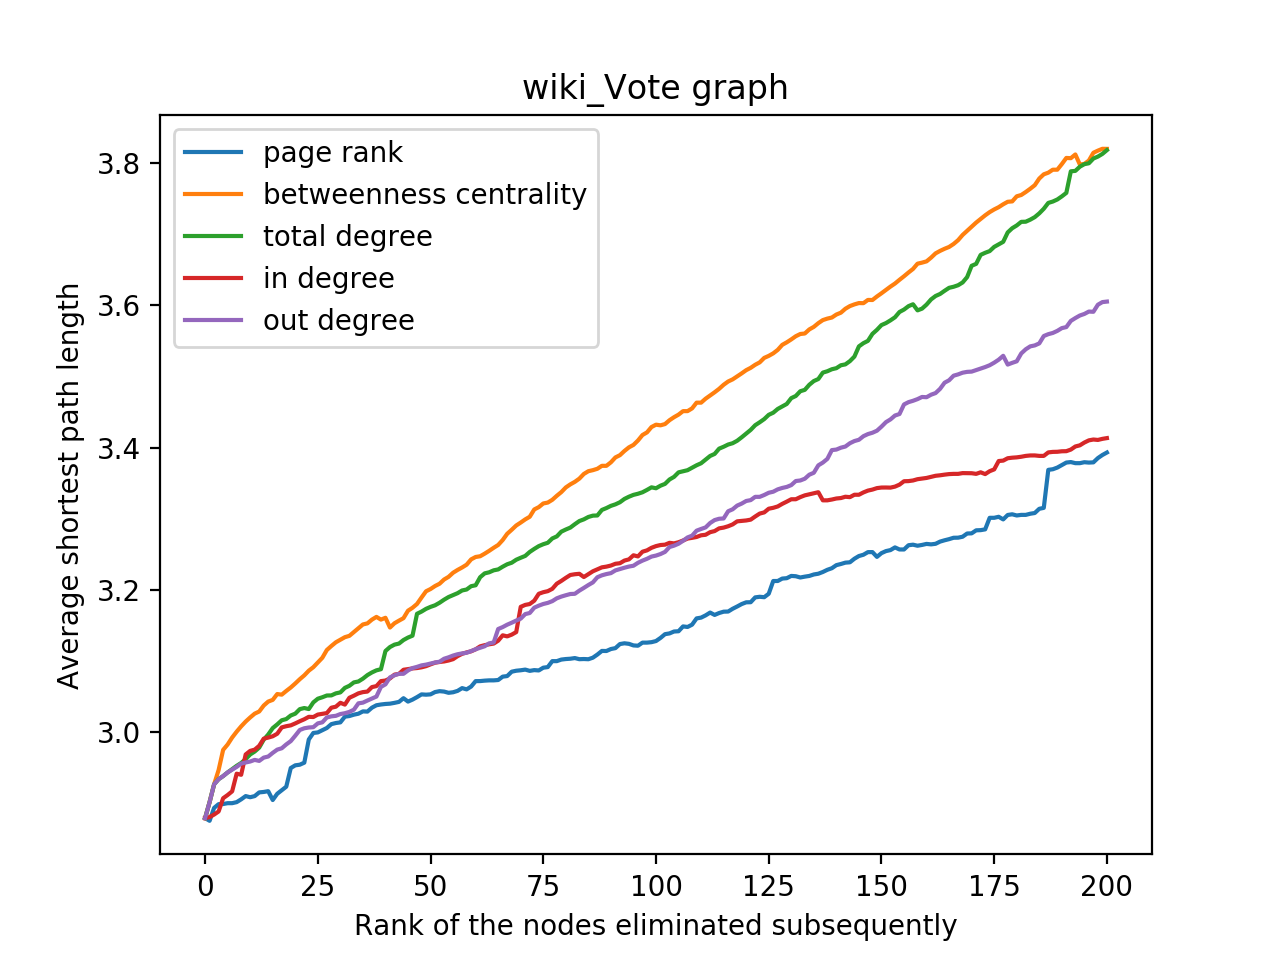
\includegraphics[width=10cm, height=8cm]{final_images/wikivote.png}
\label{wikivote_elim}
\caption{Real graph node elimination effect on ASPL.}
\end{figure}

\par Figure \ref{wikivote_elim} shows that PageRank is the worst in measuring the significance of ASPL, while both betweenness centrality and total degree perform well with the former slightly better. The trend and relative ranking in Figure \ref{wiki_vote} is consistent with previous simulation results given the similar degree dependence level. \\ 

\item Node Elimination Effect on Simulated Model of Wiki-Vote \\

\par We further generate the theoretical model to fit Wiki-vote network. From \ref{wikivote_stats} and \hyperlink{powerlaw_fit}{tail-distribution fitting}, we have parameters:  $\alpha$ = 3.5, $\beta$ = 2.5,  E = 14.57, d = 0.339 and n = 7115. 
\par Note that there exists inflexible difference between fitting model and real graph. Specifically the clustering coefficient, the real data has average clustering coefficients of 0.1409, while the simulation graph is just in the level of 0.005. This time, we repeat the model simulation for 10 times and measure the effect upon ASPL for consecutively 200 nodes. As before, we take the average to reduce the noise. 

\begin{figure}[!htbp]
\label{wikisim}
\centering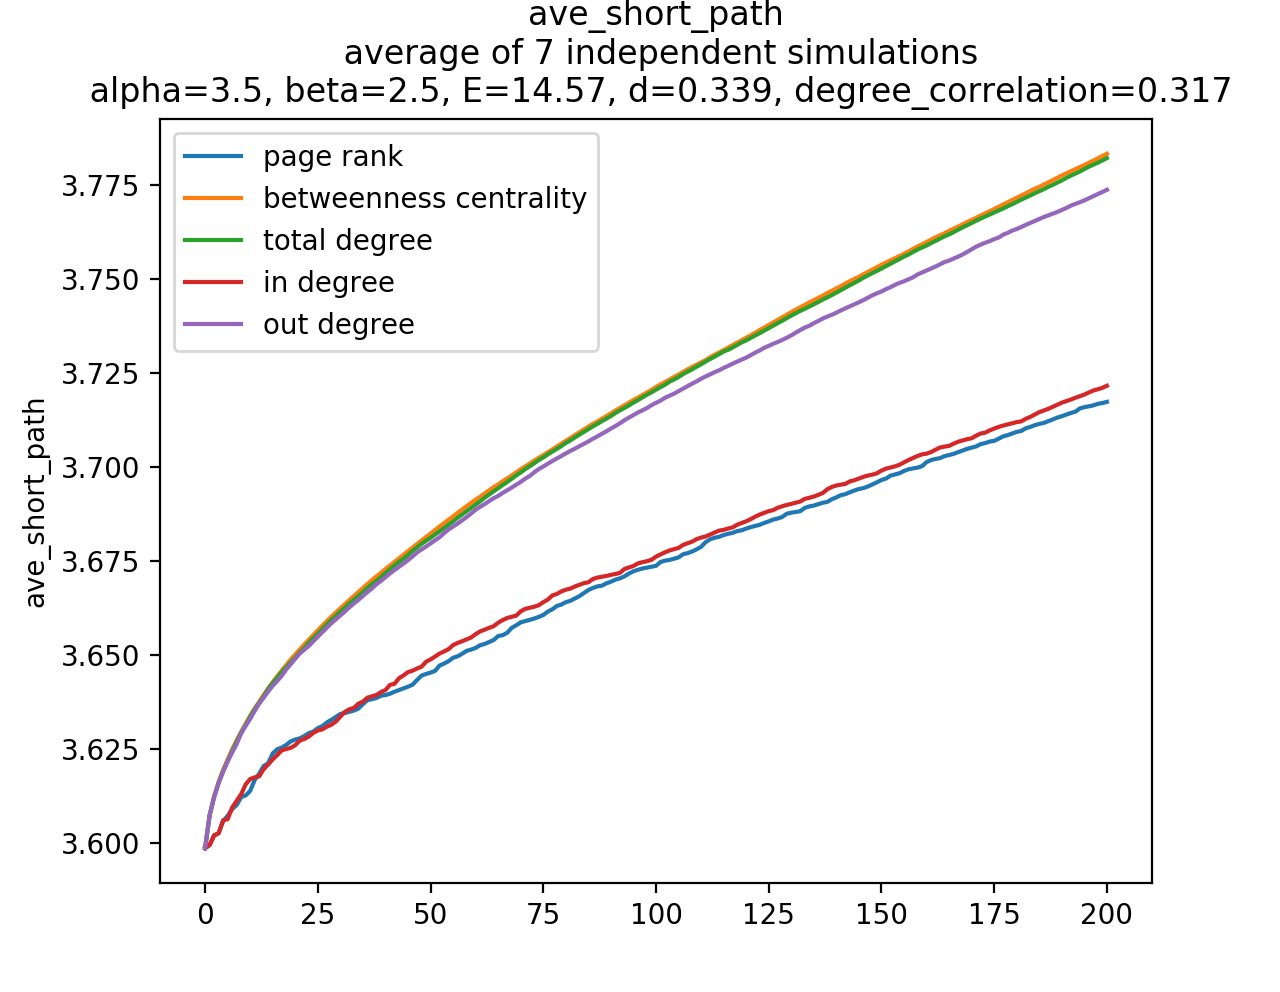
\includegraphics[width=10cm, height=8cm]{final_images/wikisim.png}
\caption{Fitting model average effect on average shortest path length.}
\end{figure}

From Figure \ref{wikisim},  we could see the result is generally similar with the real data in \ref{wikivote_elim} with same ranking of measures' performance: BC--total degree--out-degree-in-degree--PR.
\par Nevertheless, there is some difference:
\begin{enumerate}
\item  In the case of simulation model, the effect of total degree is almost the same as that of betweenness centrality, whereas in Wiki-vote network betweenness is better.
\item  n the case of simulation model, the effect of in-degree is close to, but slightly better than, PageRank, while in Wiki-vote network the difference is bigger.
\item Wiki-vote network has larger range of ASPL (2.8 to 3.8), while in simulation model it is 3.6 to 3.8. The potential explanation may be that the simulated graph presents the average situation, which reflecting the expected effect, in contrast, the real graph is a sample realization, it has more noise.
\end{enumerate}

\end{enumerate}

\subsection{Conlusions}
\begin{enumerate}
\item In general, BC and total degree mostly affect ASPL, while PR is the worst indicator, with in-degree and out-degree in between.
\item Dependence (degree correlation) level affects the relarive ranking of the effects of each measures. Specifically, the more correlated is in-degree and out-degree sequence, the smaller their differences.
\end{enumerate}


\section{Appendix}
\begin{enumerate}
\item  \hypertarget{pf_of_dependency}{Proof of Dependencies of Parameters:} \\
From the relationship between $W^{+}$ and $W^{-}$: 
  \begin{align*}
 W^{+} = a \cdot d \cdot{W^{-}}^{s} + a \cdot (1-d) \cdot {\hat{W^{-}}} ^{s} 
 \end{align*}
 where $\hat{W^{-}}$ is the independent copy of $W^{-}$. Applying the double integral, the probability of $W^{+}$ is thus the following:
  \begin{align*}
 P( W^{+} > x ) & = P( d \cdot{W^{-}}^{s} + (1 - d) \cdot {\hat{W^{-}}} ^{s} > \frac{x}{a} ) \\
          & =  {(\frac{c_{1}}{c})}^{-\beta} +  {(\frac{c_{2}}{c})}^{-\beta} -  {(\frac{ c_{1}c_{2}   }{ c^{2} })}^{-\beta}
 \end{align*}
 
 where $c_{1}$ is the integral boundary value for $W^{-}$: $c_{1} = {\frac{1}{d}}^{\frac{1}{s}} \cdot {( \frac{x}{a} - (1-d) \cdot c^{s})}^{\frac{1}{s}}$; and $c_{2}$ for $\hat{W^{-}}$: 
 $c_{2} = {\frac{1}{1-d}}^{\frac{1}{s}} \cdot {( \frac{x}{a} - d \cdot c^{s})}^{\frac{1}{s}}$. Hence the power law distribution:
 \begin{align*}
\lim_{x \rightarrow +\infty } \frac{ {(\frac{c_{1}}{c})}^{-\beta} +  {(\frac{c_{2}}{c})}^{-\beta} -  {(\frac{ c_{1}c_{2}   }{ c^{2} })}^{-\beta}  }{x^{-\alpha}} = Constant
\end{align*}
 \quad\\

To satisfy the power law requirement, it suffices that:
  \begin{align*}
  s = \frac{\beta} {\alpha} 
 \end{align*}
 \quad\\
 By definition, the lower bound for $W^{+}$ is $b$ and the lower bound for $W^-$ and $\hat{W}^-$ is $c$, so we have:
   \begin{align*}
  b = a \cdot d \cdot c^{s} + a \cdot (1-d) \cdot c^{s} = a \cdot c^{s}
 \end{align*}
 
 Additionally, as the mean of in-degree should be equal to that of out-degree, we have: 
  \begin{align*}
  E(W^{+}) = E(W^{-})  & \Rightarrow    a \cdot E({W^{-}}^{s}) = E({W^{-}}^{s})  \\
 & \Rightarrow    a \cdot \frac{\beta}{\beta - s} \cdot c^{s} = \frac{\beta}{\beta-1} \cdot c  
 \end{align*}
 Specifically in consideration of the case where s = 1, given that case in-degree and out-degree are supposed to be equal, thus identical $W^{+}$ and $W^{-}$, a should also be 1.

\item \hypertarget{eaual_sum_algo}{Sequence-modification algorithm}
\par Given the in-out degree distribution from realized $W^{+}$ and $W^{-}$, we generate the modified in-out degree sequence satisfying equal sum of in-out degree sequence while approximately maintaining the previous distribution.\\
 In the first place, we derive the constant value $\kappa$. 
% kappa-definition
\begin{align*}
 \kappa = min\{ 1 - \alpha^{-1}, 1 - \beta^{-1}, \frac{1}{2} \}
 \end{align*}

% algorithm
\begin{steps} 
 \item  Fix $0 < \delta_{0} < \kappa$, specifically choose $\delta_{0} = 0.995 * \kappa$ 
 \item  Sample an i.i.d. sequence $\{ \gamma_{1},\cdots, \gamma_{n} \}$ from in-degree distribution the poisson of $W^{+}$; let $\Gamma_{n} = \sum_{i = 1}^{n} \gamma_{i} $ 
 \item Sample an i.i.d. sequence $\{ \xi_{1},\cdots, \xi_{n} \}$ from out-degree distribution the poisson of $W^{-}$; let $\Xi_{n} = \sum_{i = 1}^{n} \xi_{i} $ 
 \item Define $\Delta_{n} = \Gamma_{n} - \Xi_{n}$, If $ \lvert \Delta_{n} \rvert  \leq n^{1 - \kappa + \delta_{0}}$ proceed to step 5; otherwise repeat from step 2.
 
 \end{steps}

\item TODO: a github repo includes readme.md(introduce how to use the codes?), codes, excel fiels (with specifications) , etc.

\end{enumerate}

\begin{thebibliography}{1}

  \bibitem{algo} Ningyuan Chen and Mariana Olvera-Cravioto,
   \emph{ Directed Random Graphs with
Given Degree Distributions July 12, 2012
 } 
\url{https://arxiv.org/pdf/1207.2475.pdf}
 
 \bibitem{git} 
 \text{Project's GitHub page} 
 \url{https://github.com/leahwu/Go_graphs}
 
 
 \bibitem{networkx} 
 \text{networkx package}
  \url{https://networkx.github.io/documentation/networkx-1.11/} 
  Released Jan 30, 2016
 
 \bibitem{dcm}
 \text{directed\_configuraiton\_model}
  \url{https://networkx.github.io/documentation/networkx-1.11/reference/generated/networkx.generators.degree_seq.directed_configuration_model.html?highlight=directed
  %20configuration%20model#networkx.generators.degree_seq.directed_configuration_model}
  
\bibitem{pr_algo1}
\text{A. Langville and C. Meyer, “A survey of eigenvector methods of web information retrieval.”}
\url{ http://citeseer.ist.psu.edu/713792.html}  

\bibitem{pr_algo2}
\text{Page, Lawrence; Brin, Sergey; Motwani, Rajeev and Winograd, Terry, The PageRank citation ranking: Bringing order to the Web. 1999}
\url{http://dbpubs.stanford.edu:8090/pub/showDoc.Fulltext?lang=en&doc=1999-66&format=pdf}

\bibitem{bc_algo1}
\text{Ulrik Brandes: A Faster Algorithm for Betweenness Centrality. Journal of Mathematical Sociology 25(2):163-177, 2001.}
\url{http://www.inf.uni-konstanz.de/algo/publications/b-fabc-01.pdf}

\bibitem{bc_algo2}
\text{(1, 2) Ulrik Brandes: On Variants of Shortest-Path Betweenness Centrality and their Generic Computation. Social Networks 30(2):136-145, 2008.}
\url{http://www.inf.uni-konstanz.de/algo/publications/b-vspbc-08.pdf}

\bibitem{bc_algo3}
\text{Ulrik Brandes and Christian Pich: Centrality Estimation in Large Networks. International Journal of Bifurcation and Chaos 17(7):2303-2318, 2007.}
\url{http://www.inf.uni-konstanz.de/algo/publications/bp-celn-06.pdf}

\bibitem{bc_algo3}
\text{Linton C. Freeman: A set of measures of centrality based on betweenness. Sociometry 40: 35–41, 1977}
\url{http://moreno.ss.uci.edu/23.pdf}
  
  \bibitem{spearman}
  Spearman's ranking coefficient
  \url{https://en.wikipedia.org/wiki/Spearman%27s_rank_correlation_coefficient}
  
  \bibitem{wikivote_source}
  Wiki-vote website and data
\url{https://snap.stanford.edu/data/wiki-Vote.html}

  \end{thebibliography}



\end{document}


